% Options for packages loaded elsewhere
\PassOptionsToPackage{unicode}{hyperref}
\PassOptionsToPackage{hyphens}{url}
\PassOptionsToPackage{dvipsnames,svgnames,x11names}{xcolor}
%
\documentclass[
  11pt,
]{article}
\usepackage{amsmath,amssymb}
\usepackage{iftex}
\ifPDFTeX
  \usepackage[T1]{fontenc}
  \usepackage[utf8]{inputenc}
  \usepackage{textcomp} % provide euro and other symbols
\else % if luatex or xetex
  \usepackage{unicode-math} % this also loads fontspec
  \defaultfontfeatures{Scale=MatchLowercase}
  \defaultfontfeatures[\rmfamily]{Ligatures=TeX,Scale=1}
\fi
\usepackage{lmodern}
\ifPDFTeX\else
  % xetex/luatex font selection
\fi
% Use upquote if available, for straight quotes in verbatim environments
\IfFileExists{upquote.sty}{\usepackage{upquote}}{}
\IfFileExists{microtype.sty}{% use microtype if available
  \usepackage[]{microtype}
  \UseMicrotypeSet[protrusion]{basicmath} % disable protrusion for tt fonts
}{}
\makeatletter
\@ifundefined{KOMAClassName}{% if non-KOMA class
  \IfFileExists{parskip.sty}{%
    \usepackage{parskip}
  }{% else
    \setlength{\parindent}{0pt}
    \setlength{\parskip}{6pt plus 2pt minus 1pt}}
}{% if KOMA class
  \KOMAoptions{parskip=half}}
\makeatother
\usepackage{xcolor}
\usepackage[margin=24mm]{geometry}
\usepackage{color}
\usepackage{fancyvrb}
\newcommand{\VerbBar}{|}
\newcommand{\VERB}{\Verb[commandchars=\\\{\}]}
\DefineVerbatimEnvironment{Highlighting}{Verbatim}{commandchars=\\\{\}}
% Add ',fontsize=\small' for more characters per line
\newenvironment{Shaded}{}{}
\newcommand{\AlertTok}[1]{\textcolor[rgb]{1.00,0.00,0.00}{\textbf{#1}}}
\newcommand{\AnnotationTok}[1]{\textcolor[rgb]{0.38,0.63,0.69}{\textbf{\textit{#1}}}}
\newcommand{\AttributeTok}[1]{\textcolor[rgb]{0.49,0.56,0.16}{#1}}
\newcommand{\BaseNTok}[1]{\textcolor[rgb]{0.25,0.63,0.44}{#1}}
\newcommand{\BuiltInTok}[1]{\textcolor[rgb]{0.00,0.50,0.00}{#1}}
\newcommand{\CharTok}[1]{\textcolor[rgb]{0.25,0.44,0.63}{#1}}
\newcommand{\CommentTok}[1]{\textcolor[rgb]{0.38,0.63,0.69}{\textit{#1}}}
\newcommand{\CommentVarTok}[1]{\textcolor[rgb]{0.38,0.63,0.69}{\textbf{\textit{#1}}}}
\newcommand{\ConstantTok}[1]{\textcolor[rgb]{0.53,0.00,0.00}{#1}}
\newcommand{\ControlFlowTok}[1]{\textcolor[rgb]{0.00,0.44,0.13}{\textbf{#1}}}
\newcommand{\DataTypeTok}[1]{\textcolor[rgb]{0.56,0.13,0.00}{#1}}
\newcommand{\DecValTok}[1]{\textcolor[rgb]{0.25,0.63,0.44}{#1}}
\newcommand{\DocumentationTok}[1]{\textcolor[rgb]{0.73,0.13,0.13}{\textit{#1}}}
\newcommand{\ErrorTok}[1]{\textcolor[rgb]{1.00,0.00,0.00}{\textbf{#1}}}
\newcommand{\ExtensionTok}[1]{#1}
\newcommand{\FloatTok}[1]{\textcolor[rgb]{0.25,0.63,0.44}{#1}}
\newcommand{\FunctionTok}[1]{\textcolor[rgb]{0.02,0.16,0.49}{#1}}
\newcommand{\ImportTok}[1]{\textcolor[rgb]{0.00,0.50,0.00}{\textbf{#1}}}
\newcommand{\InformationTok}[1]{\textcolor[rgb]{0.38,0.63,0.69}{\textbf{\textit{#1}}}}
\newcommand{\KeywordTok}[1]{\textcolor[rgb]{0.00,0.44,0.13}{\textbf{#1}}}
\newcommand{\NormalTok}[1]{#1}
\newcommand{\OperatorTok}[1]{\textcolor[rgb]{0.40,0.40,0.40}{#1}}
\newcommand{\OtherTok}[1]{\textcolor[rgb]{0.00,0.44,0.13}{#1}}
\newcommand{\PreprocessorTok}[1]{\textcolor[rgb]{0.74,0.48,0.00}{#1}}
\newcommand{\RegionMarkerTok}[1]{#1}
\newcommand{\SpecialCharTok}[1]{\textcolor[rgb]{0.25,0.44,0.63}{#1}}
\newcommand{\SpecialStringTok}[1]{\textcolor[rgb]{0.73,0.40,0.53}{#1}}
\newcommand{\StringTok}[1]{\textcolor[rgb]{0.25,0.44,0.63}{#1}}
\newcommand{\VariableTok}[1]{\textcolor[rgb]{0.10,0.09,0.49}{#1}}
\newcommand{\VerbatimStringTok}[1]{\textcolor[rgb]{0.25,0.44,0.63}{#1}}
\newcommand{\WarningTok}[1]{\textcolor[rgb]{0.38,0.63,0.69}{\textbf{\textit{#1}}}}
\usepackage{longtable,booktabs,array}
\usepackage{calc} % for calculating minipage widths
% Correct order of tables after \paragraph or \subparagraph
\usepackage{etoolbox}
\makeatletter
\patchcmd\longtable{\par}{\if@noskipsec\mbox{}\fi\par}{}{}
\makeatother
% Allow footnotes in longtable head/foot
\IfFileExists{footnotehyper.sty}{\usepackage{footnotehyper}}{\usepackage{footnote}}
\makesavenoteenv{longtable}
\usepackage{graphicx}
\makeatletter
\def\maxwidth{\ifdim\Gin@nat@width>\linewidth\linewidth\else\Gin@nat@width\fi}
\def\maxheight{\ifdim\Gin@nat@height>\textheight\textheight\else\Gin@nat@height\fi}
\makeatother
% Scale images if necessary, so that they will not overflow the page
% margins by default, and it is still possible to overwrite the defaults
% using explicit options in \includegraphics[width, height, ...]{}
\setkeys{Gin}{width=\maxwidth,height=\maxheight,keepaspectratio}
% Set default figure placement to htbp
\makeatletter
\def\fps@figure{htbp}
\makeatother
\setlength{\emergencystretch}{3em} % prevent overfull lines
\providecommand{\tightlist}{%
  \setlength{\itemsep}{0pt}\setlength{\parskip}{0pt}}
\setcounter{secnumdepth}{5}
\newlength{\cslhangindent}
\setlength{\cslhangindent}{1.5em}
\newlength{\csllabelwidth}
\setlength{\csllabelwidth}{3em}
\newlength{\cslentryspacingunit} % times entry-spacing
\setlength{\cslentryspacingunit}{\parskip}
\newenvironment{CSLReferences}[2] % #1 hanging-ident, #2 entry spacing
 {% don't indent paragraphs
  \setlength{\parindent}{0pt}
  % turn on hanging indent if param 1 is 1
  \ifodd #1
  \let\oldpar\par
  \def\par{\hangindent=\cslhangindent\oldpar}
  \fi
  % set entry spacing
  \setlength{\parskip}{#2\cslentryspacingunit}
 }%
 {}
\usepackage{calc}
\newcommand{\CSLBlock}[1]{#1\hfill\break}
\newcommand{\CSLLeftMargin}[1]{\parbox[t]{\csllabelwidth}{#1}}
\newcommand{\CSLRightInline}[1]{\parbox[t]{\linewidth - \csllabelwidth}{#1}\break}
\newcommand{\CSLIndent}[1]{\hspace{\cslhangindent}#1}
\ifLuaTeX
\usepackage[bidi=basic]{babel}
\else
\usepackage[bidi=default]{babel}
\fi
\babelprovide[main,import]{brazilian}
% get rid of language-specific shorthands (see #6817):
\let\LanguageShortHands\languageshorthands
\def\languageshorthands#1{}
\ifLuaTeX
  \usepackage{selnolig}  % disable illegal ligatures
\fi
\IfFileExists{bookmark.sty}{\usepackage{bookmark}}{\usepackage{hyperref}}
\IfFileExists{xurl.sty}{\usepackage{xurl}}{} % add URL line breaks if available
\urlstyle{same}
\hypersetup{
  pdftitle={Relatório técnico estendido: PG Information and Control Frontier --- núcleo parcial},
  pdfauthor={Walter Yanko de Aragão Brandão},
  pdflang={pt-BR},
  colorlinks=true,
  linkcolor={Maroon},
  filecolor={Maroon},
  citecolor={Blue},
  urlcolor={Blue},
  pdfcreator={LaTeX via pandoc}}

\title{Relatório técnico estendido: PG Information and Control Frontier
--- núcleo parcial}
\author{Walter Yanko de Aragão Brandão}
\date{20 October 2026}

\begin{document}
\maketitle

\hypertarget{resumo}{%
\section{Resumo}\label{resumo}}

Este estudo computacional investiga limites de informação e decisão em
um modelo recuperado de reator de propilenoglicol de seis estados.
Existe uma classe química exatamente indistinguível de dimensão dois sob
capacidades caloríficas constantes e cinética de primeira ordem.
Acrescentar realimentação térmica da camisa não a elimina. O posto
funcional das capacidades caloríficas caracteriza uma ambiguidade
suficiente remanescente; exemplos com propriedades dependentes de
temperatura examinam a separabilidade prática. A suíte principal
executou 5320 trajetórias, com 400 trajetórias de confirmação em
sementes independentes e 18 verificações de grade. Na diluição nominal,
separação inicial de produto de 0,8 kmol/m3 implica limite inferior de
0.060376 kmol h/m3 para o pior IAE entre dois mundos em 0,9 h. Há
conflito decisório positivo em 51 dos 80 casos finitos examinados. Os
ganhos médios adicionais por ambiguidade foram 0,63\% e 0,66\%, com
intervalos pareados incluindo zero; compartilhar a correção com o
preditor reduziu IAE em 39,91\% frente à correção somente do estimador.
Não se demonstrou superioridade sobre todo NMPC contínuo. As
alternativas físicas não foram calibradas, e os números históricos ICAC
não foram reproduzidos independentemente. Trata-se de manuscrito parcial
de pesquisa, ainda não validado para submissão. \# Introdução

O controle inferencial de qualidade depende da informação carregada
pelos sensores e das previsões usadas na escolha das ações. Reduzir o
RMSE de concentração não garante diminuir a perda de controle em malha
fechada. Este estudo audita um CSTR de propilenoglicol de seis estados
antes de testar maior complexidade. Separam-se duas perguntas: existe
ambiguidade química demonstrável quando somente temperaturas são
medidas? Representar essa ambiguidade melhora o controle contra
comparadores igualmente informados?

O manuscrito interno ICAC já descrevia gêmeos calorimétricos e conflitos
de decisão. Seus percentuais permanecem evidência histórica. A branch e
o arquivo completo de reprodução ICAC não estavam disponíveis. O
presente manuscrito registra um núcleo computacional independente, com
pendências explícitas para publicação.

\hypertarget{trabalhos-relacionados}{%
\section{Trabalhos relacionados}\label{trabalhos-relacionados}}

Observabilidade e identificabilidade não lineares distinguem perda de
informação de dificuldade numérica (Hermann e Krener 1977; Villaverde,
Barreiro, e Papachristodoulou 2016). Ambiguidade de concentração em
reatores já aparece em estudos de cinética não monotônica e controle por
saída (Schaum et al. 2007). Sensibilidades empíricas revelam direções
fracas sem demonstrar observabilidade estrutural global (Lall, Marsden,
e Glavaski 2002).

MHE com restrições e MPC por realimentação de saída possuem
fundamentação consolidada (Rao, Rawlings, e Mayne 2003; Rawlings, Mayne,
e Diehl 2017). Regret sob medições possui antecedentes com comparadores
diferentes, em sistemas lineares (Goel e Hassibi 2021). Predição
orientada à decisão e controle dual também antecedem a campanha
(Elmachtoub e Grigas 2022; Klenske e Hennig 2016). Preprints recentes
investigam medições dependentes de entrada e risco de parâmetros
latentes (Cao et al. 2026; Enwerem, Baras, e Belta 2026). A contribuição
candidata aqui é a classificação específica pela capacidade calorífica,
com proveniência rastreável e experimentos de decisão no PG.

\hypertarget{modelo-fuxedsico-do-processo}{%
\section{Modelo físico do processo}\label{modelo-fuxedsico-do-processo}}

As fontes são a dissertação de Brandão e seu modelo MATLAB recuperado
(Brandao 2019). A reação é A+B para C; metanol M é tratado como inerte.
O volume é constante, com saída regulada pelo nível. Usam-se kmol/m3,
kelvin, horas e kJ:
\[v=F_A/\rho_A+F_B/\rho_B+F_M/\rho_M,\quad D=v/V,\quad
r=k_0\exp[-E/(R(T+0.183333333333))]C_A.\] Os balanços são
\[\dot C_A=F_A/V-DC_A-r,\qquad\dot C_B=F_B/V-DC_B-r,\]
\[\dot C_C=-DC_C+r,\qquad\dot C_M=F_M/V-DC_M.\] Definindo
\(W=\sum_i c_{p,i}C_i\) e \(F_{cp}=F_Ac_{p,A}+F_Bc_{p,B}+F_Mc_{p,M}\):
\[Q=m_wc_{p,B}(T_a-T)[1-e^{-UA/(m_wc_{p,B})}],\]
\[\dot T=\frac{Q+F_{cp}(T_0-T)-\Delta H_r rV}{VW},\qquad
\dot T_t=\frac{m_wc_{p,B}(T_a-T_t)-Q}{\rho_BV_tc_{p,B}}.\] Somente
\(T,T_t\) são medidas. A entrada otimizada é \(m_w=q\,453.59237\)
kmol/h; as alimentações atuais são conhecidas, sem antecipação de
perturbações. Preserva-se a assimetria histórica: \(T_t\) não aparece em
\(Q\).

A entalpia executável é -83736 kJ/kmol, enquanto a tabela da dissertação
informa -91556.90. A conversão imperial arredondada e o deslocamento de
Arrhenius são convenções preservadas para reprodução. O exemplo público
de Fogler contém correção da entalpia com temperatura, mas utiliza
outras condições operacionais (Fogler, s.d.); não autoriza substituir
constantes sem calibração.

Um caso didático relacionado utiliza cinética de primeira ordem com água
em excesso e líquido não ideal (Chan e Seider 2004). Isso sustenta a
aproximação cinética como benchmark, mas impede tratar apenas a
calorimetria ideal como validação da equivalência física de inventários
reais.

O benchmark de volume constante calcula a vazão volumétrica de saída
pelas densidades das alimentações, mas não impõe equação de estado
dependente da composição nem fechamento por volumes molares parciais a
cada inventário candidato. Positividade representa admissibilidade no
modelo, não admissibilidade física completa da mistura líquida.
Restrições exatas adicionais de composição e volume intersectariam o
subespaço invisível e poderiam reduzi-lo. Variação de volume pela reação
e entalpia não ideal permanecem fora das reconciliações testadas.

\hypertarget{alternativas-fuxedsicas-expluxedcitas}{%
\subsection{Alternativas físicas
explícitas}\label{alternativas-fuxedsicas-expluxedcitas}}

M1H introduz consistência de Kirchhoff:
\(\Delta H_r(T)=\Delta H_r(T_r)+\int_{T_r}^T(c_{p,C}-c_{p,A}-c_{p,B})\,d\theta\),
assumindo a entalpia histórica na temperatura nominal
\(T_r=332.333618020\) K. Essa referência não é conhecida
independentemente. M1J acrescenta \(Q=G(T_t-T)\) com armazenamento
térmico da camisa. Escolhe-se
\(G=m_{w0}c_{p,B}[\exp(UA/(m_{w0}c_{p,B}))-1]\) para igualar a remoção
estacionária nominal. Não se confunde UA de uma serpentina com
condutância de uma camisa perfeitamente misturada.

M2L e M2Q adotam \(c_{p,i}(T)=a_i+b_i(T-T_r)+c_i(T-T_r)^2\), com \(a_i\)
históricos. As inclinações relativas são (0.0015,0.0002,0.0025,0.0010)
por K; as curvaturas relativas são
(0.000010,0.000002,0.000016,-0.000003) por K ao quadrado. M2L anula as
curvaturas. Entalpias sensíveis e de reação são integradas
consistentemente. São modelos sintéticos de sensibilidade, sem
calibração de propriedades; nenhum constitui o M1 fisicamente validado
solicitado na missão integral.

\hypertarget{arquiteturas-de-estimauxe7uxe3o-e-controle}{%
\section{Arquiteturas de estimação e
controle}\label{arquiteturas-de-estimauxe7uxe3o-e-controle}}

B1 combina UKF de seis estados e preditor nominal. B2\_estimator
acrescenta fatores logarítmicos de cinética e troca térmica ao UKF,
preservando o preditor nominal. B2\_both transmite esses fatores
estimados ao preditor. Nenhum recebe parâmetros verdadeiros. B0 é um PI
documentado sobre concentração inferida, com ganhos 4 e 2 e antiwindup;
não é reprodução de uma cascata histórica otimamente sintonizada.

B3\_assumed\_inventory impõe inventários iniciais nominais.
B3\_known\_inventory recebe os inventários verdadeiros uma única vez e
dispõe de informação adicional. Os estados reduzidos são
\((C_C,T,T_t)\), com totais propagados pelos balanços de alimentação e
diluição. B4 é MHE determinístico de seis passos, prior aproximado de
chegada, sem variáveis de ruído de processo e orçamento de 18
avaliações. B5 usa estado atual verdadeiro somente como oráculo
diagnóstico, mantendo parâmetros nominais no preditor.

P1 minimiza custo médio de três representantes. P2 minimiza seu maior
regret. P3 combina essa regra com adaptação causal de parâmetros. P4
aplica ação robusta quando os representantes discordam em pelo menos 0,2
unidade nominal de refrigeração; caso contrário utiliza política nominal
adaptada. Os representantes são o ponto do UKF e compensações
calorimétricas de produto de mais/menos \(0.4e^{-\int Ddt}\). Não
constituem conjunto envolvente certificado nem amostragem posterior
completa.

As variantes P5 mantêm controle nominal e acrescentam amostra inicial;
quatro amostras periódicas; coleta por evento com cota quatro; atraso de
três passos; ruído ampliado; ou até oito amostras frequentes. O desvio
padrão de composição é 0,03 kmol/m3, ampliado para 0,15 no caso ruidoso.
Inovações atrasadas são transportadas aproximadamente pela diluição, com
incremento explícito de variância. Não há suavizador completo de
medições fora de sequência. Pedidos por evento usam largura da crença e
desacordo decisório disponíveis, sem observações futuras.

A política padrão enumera até 25 sequências de dois blocos: primeira
ação por três passos, segunda por onze. Incrementos pertencem a cinco
pontos entre -0,4 e 0,4. Todos compartilham \(0.05\le q\le3\) e variação
máxima 0,4; no cenário de saturação, o mesmo teto reduzido 1,3 vale para
todos. A restrição amostrada é \(T\le344.261111\) K. Ausência de plano
conjuntamente viável ativa contingência explícita de menor violação
prevista. Isso não estabelece segurança garantida.

O custo adimensional é
\[J=\sum_{j=1}^{14}\left[0.8\left(\frac{C_{C,j}-r_k}{2.295764605}\right)^2+
1000\left(\frac{\max(T_j-344.261111,0)}{160/1.8}\right)^2\right]
+0.2[(q_1-q_{\rm prev})^2+(q_2-q_1)^2].\] Esse objetivo difere do IAE.
B1\_continuous otimiza o mesmo problema de dois blocos por SLSQP,
iniciado na solução da grade. É um comparador local; não equivale ao
NMPC histórico completo de horizonte 57 e seis movimentos.

\hypertarget{metodologia-experimental}{%
\section{Metodologia experimental}\label{metodologia-experimental}}

O protocolo congelado prevê 14 cenários, 19 métodos e 20 sementes
pareadas por combinação. Cada trajetória contém 60 intervalos de 0,015
h, totalizando 0,9 h. Incluem-se nominal, servo, erros cinético e
térmico, inventários com sinais opostos, perturbação de alimentação,
erro de capacidade calorífica, ruído correlacionado, perda de medição,
saturação, perturbações combinadas, estado fora do conjunto inicial e
referência inalcançável. As variantes físicas estruturais são analisadas
separadamente do benchmark de controle M0.

Os desvios padrão iniciais do UKF são (0,15;0,8;0,4;0,3;0,5;0,5). A
diagonal de Q é (2e-6;2e-5;2e-6;1e-7;0,015;0,006). Os ruídos térmicos
possuem desvios (1,385;1,062)/1,8 K. Fatores adaptativos têm variância
inicial 0,15 ao quadrado, variância de processo 1e-5 e limites
{[}-0,5;0,5{]}. Usam-se alpha=0,5 e beta=2. Nenhuma sintonia utiliza
desfechos reservados.

As sementes principais são 4100--4119; a confirmação 8100--8119 cobre
quatro cenários declarados e cinco métodos. As sementes 101--103 avaliam
uma grade mais densa; a semente 11 serve ao piloto de custo. Os ruídos
são pareados entre métodos. O bootstrap reamostra sementes; para a suíte
finita, cada semente é primeiro agregada entre cenários. A incerteza
descreve essa suíte, sem representar uma população industrial. Três
contrastes primários recebem ajuste de Holm; os demais permanecem
exploratórios.

A planta usa RK4 com 12 subpassos, comparado ao DOP853 do SciPy com rtol
2e-11 e atol 1e-12. Predição usa três subpassos e filtro quatro. Estados
físicos não são recortados. Reparos de positividade e covariância do
estimador são contabilizados. Métricas escalares são recalculadas
independentemente das trajetórias salvas. Os tempos pertencem a CPU
Linux hospedada, sem certificação no Ryzen de destino.

\hypertarget{paruxe2metros-e-condiuxe7uxe3o-inicial}{%
\section{Parâmetros e condição
inicial}\label{paruxe2metros-e-condiuxe7uxe3o-inicial}}

\begin{longtable}[]{@{}lll@{}}
\toprule\noalign{}
Parameter & Value & Unit \\
\midrule\noalign{}
\endhead
\bottomrule\noalign{}
\endlastfoot
V & 1.89183 & m3 \\
Vt & 1.10011 & m3 \\
UA & 30385.6 & kJ/(h K) \\
CpA & 146.538 & kJ/(kmol K) \\
CpB & 75.3624 & kJ/(kmol K) \\
CpC & 192.593 & kJ/(kmol K) \\
CpM & 81.6426 & kJ/(kmol K) \\
E & 75362.4 & kJ/kmol \\
R & 8.31917 & kJ/(kmol K) \\
k0 & 1.696e+13 & 1/h \\
DeltaH & -83736 & kJ/kmol \\
FA & 36.2874 & kmol/h \\
FB & 453.592 & kmol/h \\
FM & 45.3592 & kmol/h \\
mw0 & 453.592 & kmol/h \\
T0 & 297.039 & K \\
Ta & 288.706 & K \\
\end{longtable}

Equilíbrio nominal: 0.607024732, 33.989102107, 2.295764605, 3.628486671,
332.333618020, 314.397585330.

\hypertarget{escopo-matemuxe1tico-e-demonstrauxe7uxf5es}{%
\section{Escopo matemático e
demonstrações}\label{escopo-matemuxe1tico-e-demonstrauxe7uxf5es}}

Os resultados seguintes descrevem a classe de modelos explicitada, sem
estabelecer validação de uma instalação industrial. O tempo é medido em
horas. Os mundos comparados compartilham alimentações conhecidas,
parâmetros, referência, restrições de atuação e temperaturas iniciais
medidas. As condições químicas iniciais pertencem ao domínio positivo
aberto admitido pelo benchmark de seis estados, sem impor uma equação de
estado validada da mistura. Restrições exatas adicionais de
admissibilidade devem ser intersectadas com a classe construída e podem
reduzir sua dimensão. Supõem-se existência e unicidade das soluções no
horizonte considerado. As entradas podem depender causalmente das
temperaturas medidas. As afirmações de informação exata usam medições
sem ruído ou acoplamento com a mesma realização aditiva de ruído.

\hypertarget{proposiuxe7uxe3o-1-classe-de-equivaluxeancia-calorimuxe9trica}{%
\subsection{Proposição 1: classe de equivalência
calorimétrica}\label{proposiuxe7uxe3o-1-classe-de-equivaluxeancia-calorimuxe9trica}}

Considere \(\dot c=F/V-D(t)c+\nu r\), com \(\nu=(-1,-1,1,0)^T\) e
\(r=k(T)C_A\). Suponha que a composição afete a dinâmica térmica somente
por \(C_A\) e \(W(T,c)=\sum_i c_{p,i}(T)C_i\). A troca térmica pode ser
qualquer função localmente Lipschitz de \(T,T_t,u\), independente das
demais coordenadas químicas. A entalpia de reação pode depender da
temperatura.

Para capacidades caloríficas constantes, dois estados iniciais que
satisfaçam \[\delta C_A=0,\quad\delta T=\delta T_t=0,\qquad
c_{p,B}\delta C_B+c_{p,C}\delta C_C+c_{p,M}\delta C_M=0\] produzem
temperaturas idênticas sob toda entrada comum admissível, enquanto ambas
as trajetórias permanecerem no domínio físico. Suas diferenças químicas
obedecem a \[\delta c(t)=e^{-\int_0^tD(s)\,ds}\delta c(0).\]

Demonstração. A igualdade de \(C_A,T\) implica igualdade das taxas de
reação. A subtração dos balanços de espécies deixa somente diluição
homogênea. A combinação calorimétrica das diferenças permanece nula;
portanto as derivadas térmicas coincidem. A unicidade das soluções
completa a demonstração. Em realimentação causal, históricos idênticos
produzem ações seguintes idênticas. Existem duas direções químicas
independentes nesse núcleo. Os seis estados livres não podem ser
reconstruídos integralmente; o subsistema que produz temperaturas possui
no máximo quatro coordenadas \((C_A,W,T,T_t)\). A construção é
suficiente para demonstrar indistinguibilidade; não caracteriza
necessariamente todos os pares indistinguíveis.

O resultado permanece com troca térmica recíproca entre camisa e reator.
Portanto a ausência de realimentação de \(T_t\) não explica,
isoladamente, a ambiguidade química bidimensional.

\hypertarget{proposiuxe7uxe3o-1b-posto-funcional-das-capacidades-caloruxedficas}{%
\subsection{Proposição 1b: posto funcional das capacidades
caloríficas}\label{proposiuxe7uxe3o-1b-posto-funcional-das-capacidades-caloruxedficas}}

Defina
\[\mathcal S=\operatorname{span}\{(c_{p,B}(T),c_{p,C}(T),c_{p,M}(T)):T\in\mathcal I\}.\]
Toda diferença com \(\delta C_A=0\) e
\((\delta C_B,\delta C_C,\delta C_M)\in\mathcal S^\perp\) admite a
construção anterior. A dimensão desse conjunto é \(3-\dim\mathcal S\).

Demonstração. A diferença de capacidade térmica é nula em toda
temperatura de \(\mathcal I\). As diferenças de espécies recebem o mesmo
fator escalar de diluição. A demonstração anterior permanece válida,
inclusive com entalpia de reação e entalpias sensíveis da alimentação
dependentes de temperatura. Capacidades constantes dão posto um. Funções
afins por espécie têm posto no máximo dois, deixando ao menos uma
direção invisível. Funções quadráticas independentes podem eliminar esse
núcleo específico. Sua eliminação NÃO demonstra observabilidade não
linear completa: podem restar outras simetrias, estados singulares e
baixa sensibilidade.

Uma consequência para instrumentação: uma medição química escalar
\(a^Tc\) resolve o produto na classe de equivalência apenas se
\[\ker(a^T|_{\mathcal N})\subseteq\ker(e_C^T|_{\mathcal N}),\] onde
\(\mathcal N\) é o subespaço químico invisível. Medir \(C_C\) satisfaz o
requisito; medir uma concentração arbitrária pode não satisfazê-lo.
Conhecer \(C_A+C_C\) também permite obter produto quando \(C_A\) é
identificado, mas seu valor inicial é informação adicional.

\hypertarget{proposiuxe7uxe3o-1c-entrada-constante-nuxe3o-informativa-e-teste-local-no-quociente}{%
\subsection{Proposição 1c: entrada constante não informativa e teste
local no
quociente}\label{proposiuxe7uxe3o-1c-entrada-constante-nuxe3o-informativa-e-teste-local-no-quociente}}

Para M0 sob entradas constantes, defina \(A=C_A\),
\(W=\sum c_{p,i}C_i\), \(q=F_A/V\), \(c=F_{cp}/V\),
\(n=c_{p,C}-c_{p,A}-c_{p,B}\), \(a(T)=[Q(T)+F_{cp}(T_0-T)]/V\) e
\(b(T)=-\Delta H_r k(T)\). Então
\(\dot A=q-(D+k)A,\quad\dot W=c-DW+nkA,\quad g=\dot T=(a+bA)/W.\) Num
ponto com \(\dot A=0\) e \(a+bA=0\), perturbações suficientemente
pequenas e arbitrárias em B, C e M mantêm A e ambas as temperaturas
constantes sob a mesma entrada fixa. Elas alteram W e decaem por
diluição. Há, portanto, três direções químicas invisíveis nesse
experimento sem excitação, embora apenas duas pertençam à família
calorimétrica válida para todas as entradas. A excitação pode distinguir
a direção adicional. Não se trata de simetria tridimensional válida para
toda entrada.

Um teste local suficiente usa os gradientes de \(T,T_t,L_fT,L_f^2T\) no
quociente \((A,W,T,T_t)\). O menor dois por dois referente a \((A,W)\) é
\(\det\begin{bmatrix}g_A&g_W\\(L_fg)_A&(L_fg)_W\end{bmatrix} =-\frac{b[bq+(D+k)a]}{W^3} +\frac{(a+bA)[-ba_T+bc+ab_T-ank]}{W^4}.\)
Obtém-se a expressão diferenciando
\(L_fg=\frac{bq+Da-bkA}{W} +\frac{(a+bA)(a_T+b_TA-c-nkA)}{W^2}.\) Menor
não nulo é condição suficiente de posto quatro nesse teste local do
quociente. Ele se anula no equilíbrio nominal com entrada constante. O
valor zero isolado não demonstra inobservabilidade; a construção
explícita de trajetórias invariantes acima demonstra esse caso
particular. O sistema de seis estados continua com posto máximo quatro
sob a simetria válida para todas as entradas. As avaliações de precisão
arbitrária são cálculos locais de apoio, não um teorema global de posto.

\hypertarget{proposiuxe7uxe3o-2-limites-de-estimauxe7uxe3o-e-rastreamento}{%
\subsection{Proposição 2: limites de estimação e
rastreamento}\label{proposiuxe7uxe3o-2-limites-de-estimauxe7uxe3o-e-rastreamento}}

Se duas concentrações possíveis no instante \(t\) têm separação
\(\Delta(t)\), qualquer estimador com o mesmo histórico informacional
fornece a mesma estimativa nos dois mundos:
\[\max_i|\hat C_C(t)-C_C^{(i)}(t)|\geq\Delta(t)/2.\] A desigualdade
triangular demonstra o resultado. O ponto médio atinge o limite quando
somente esses dois valores são possíveis.

A mesma desigualdade vale substituindo a estimativa por uma referência
comum. A integração fornece
\[\max_i\operatorname{IAE}_i(H)\geq\frac12\int_0^H\Delta(t)\,dt.\] Com
diluição constante e separação inicial \(\Delta_0\), o lado direito é
\(\Delta_0(1-e^{-DH})/(2D)\). Esse é um limite do pior erro de
rastreamento, não do regret em relação a um controlador informado do
estado. O oráculo também pode enfrentar perda transitória inevitável. A
queda do limite por diluição representa renovação física do inventário,
não informação fornecida pelo sensor.

Para entrada fixa em malha aberta e registros gaussianos com mesma
covariância conhecida \(\Sigma\), a divergência KL é
\(\frac12(\mu_1-\mu_2)^T\Sigma^{-1}(\mu_1-\mu_2)\). O risco esperado
absoluto no problema de dois mundos é limitado inferiormente por
\(\Delta(1-\mathrm{TV})/2\). Pinsker fornece
\(\Delta\max(0,1-\sqrt{\mathrm{KL}/2})/2\). A fórmula não se transfere
automaticamente para realimentação adaptativa ruidosa em que as ações
modificam a separação química. Não se reivindica aqui um limite
estocástico industrial.

\hypertarget{proposiuxe7uxe3o-3-ambiguidade-de-estado-e-conflito-decisuxf3rio}{%
\subsection{Proposição 3: ambiguidade de estado e conflito
decisório}\label{proposiuxe7uxe3o-3-ambiguidade-de-estado-e-conflito-decisuxf3rio}}

Considere custos contínuos \(J_i\) em um conjunto comum, compacto e não
vazio de sequências admissíveis \(\mathcal U\). Escreva
\(J_i^*=\min_{\mathcal U}J_i\). Então
\[\mathcal R^*=\min_{u\in\mathcal U}\max_i[J_i(u)-J_i^*]\] é zero se, e
somente se, os conjuntos de minimizadores possuem interseção não vazia.
Se não possuem, \(\mathcal R^*>0\).

Demonstração. Os regrets são não negativos. Um minimizador comum os
anula. Reciprocamente, continuidade e compacidade garantem que o mínimo
do máximo seja atingido. Se ele é zero, a decisão minimiza todos os
custos. Logo, minimizadores sem interseção implicam valor estritamente
positivo. Uma separação química grande pode coexistir com regret nulo
quando todos os mundos preferem a mesma ação, inclusive saturação comum.

Quando as restrições dependem do mundo, os ótimos individuais devem
respeitar seus conjuntos declarados e a decisão robusta pertence à
interseção. Interseção vazia significa inviabilidade, não regret finito.
O cálculo numérico marca explicitamente a ausência de candidatos
conjuntamente viáveis.

\hypertarget{proposiuxe7uxe3o-3b-quando-representar-a-ambiguidade-nuxe3o-altera-a-auxe7uxe3o-de-custo-esperado}{%
\subsection{Proposição 3b: quando representar a ambiguidade não altera a
ação de custo
esperado}\label{proposiuxe7uxe3o-3b-quando-representar-a-ambiguidade-nuxe3o-altera-a-auxe7uxe3o-de-custo-esperado}}

Nos gêmeos exatos de PG com a mesma alimentação conhecida, a vazão de
refrigeração não altera a diluição. Para qualquer plano comum, escreva
\(C_C(t;u,\delta)=C_C(t;u,0)+d(t)\delta\), onde
\(d(t)=e^{-\int_0^tD(s)ds}\) independe do plano de refrigeração. Suponha
offsets com média zero, representantes fisicamente admissíveis,
restrições dependentes apenas das temperaturas e ações comuns e custo de
tracking quadrático ponderado, acrescido de custos térmicos e de atuação
comuns. Então
\(\mathbb E_\delta J_\delta(u)=J_0(u)+\mathbb E[\delta^2]\sum_j w_jd(t_j)^2.\)
O último termo independe de \(u\). Logo, os conjuntos de minimizadores
das políticas nominal e de custo esperado são exatamente iguais, tanto
na grade quanto na classe contínua.

Demonstração. Expanda os quadrados e tome a média. O termo cruzado se
anula pela média zero; os demais custos e restrições são compartilhados.
É um caso de equivalência de certeza, não um teorema universal de
robustez. Perdas não quadráticas, diluição dependente da ação,
truncamento assimétrico de crenças, restrições físicas adicionais ou
mudança da política informacional podem invalidá-lo. No P1 de três
representantes simétricos, a proposição prevê benefício de controle
nulo, exceto por exclusões de admissibilidade e desempates numéricos.
Ela refuta a ideia de que apenas incluir esses mundos necessariamente
melhora este NMPC quadrático.

\hypertarget{proposiuxe7uxe3o-4-limite-quantitativo-condicional}{%
\subsection{Proposição 4: limite quantitativo
condicional}\label{proposiuxe7uxe3o-4-limite-quantitativo-condicional}}

Para dois custos \(\mu\)-fortemente convexos no mesmo conjunto convexo,
com minimizadores \(u_1^*,u_2^*\),
\[\mathcal R^*\geq\frac{\mu}{8}\|u_1^*-u_2^*\|^2.\] Convexidade forte e
otimalidade de primeira ordem fornecem
\(J_i(u)-J_i(u_i^*)\geq\mu\|u-u_i^*\|^2/2\). Pelo menos uma distância é
maior ou igual à metade da distância entre minimizadores. Isso demonstra
o limite. A convexidade também impede ganho por randomização sob o
máximo dos custos esperados. Essas condições NÃO foram demonstradas para
a otimização não linear de PG; nenhum regret numérico do PG é
certificado por essa expressão.

Sob indistinguibilidade exata durante todo o horizonte, uma política
causal determinística e sem ruído realiza a mesma sequência em todos os
mundos. Se suas sequências pertencem a \(\mathcal U\), seu pior regret é
pelo menos o valor minimax nesse conjunto. Uma grade finita fornece
resultado exato somente dentro da grade. Se os custos ótimos individuais
forem mantidos nos ótimos contínuos, restringir apenas as decisões
fornece limite superior do minimax contínuo. Aqui tanto as decisões
quanto os ótimos individuais são restritos à grade; o resultado não
possui, em geral, relação unilateral de limite com o regret minimax
contínuo. Não é limite inferior válido para todo controlador físico. Se
medições futuras distinguirem os mundos, regret de sequências abertas
não equivale ao valor da política adaptativa ótima.

\hypertarget{antecedentes-e-contribuiuxe7uxe3o-possuxedvel}{%
\subsection{Antecedentes e contribuição
possível}\label{antecedentes-e-contribuiuxe7uxe3o-possuxedvel}}

Observabilidade, detectabilidade, limites de risco de dois pontos,
minimax regret e estimação orientada à decisão já são conhecidos. As
demonstrações são especializações elementares, sem pretensão de uma lei
universal nova. A contribuição específica candidata é a classificação
pelo posto funcional de Cp, aplicada ao modelo PG rastreável, e a
ligação auditada entre formulação física, instrumentação e decisão.
Ainda são necessárias revisão abrangente de originalidade e propriedades
físicas calibradas.

\hypertarget{resultados-numuxe9ricos}{%
\section{Resultados numéricos}\label{resultados-numuxe9ricos}}

As comparações abaixo provêm da execução. Melhoria positiva favorece o
primeiro método. O IC da suíte reamostra 20 sementes pareadas e é
condicional aos cenários escolhidos.

\begin{longtable}[]{@{}
  >{\raggedright\arraybackslash}p{(\columnwidth - 12\tabcolsep) * \real{0.1429}}
  >{\raggedright\arraybackslash}p{(\columnwidth - 12\tabcolsep) * \real{0.1429}}
  >{\raggedright\arraybackslash}p{(\columnwidth - 12\tabcolsep) * \real{0.1429}}
  >{\raggedright\arraybackslash}p{(\columnwidth - 12\tabcolsep) * \real{0.1429}}
  >{\raggedright\arraybackslash}p{(\columnwidth - 12\tabcolsep) * \real{0.1429}}
  >{\raggedright\arraybackslash}p{(\columnwidth - 12\tabcolsep) * \real{0.1429}}
  >{\raggedright\arraybackslash}p{(\columnwidth - 12\tabcolsep) * \real{0.1429}}@{}}
\toprule\noalign{}
\begin{minipage}[b]{\linewidth}\raggedright
candidate
\end{minipage} & \begin{minipage}[b]{\linewidth}\raggedright
baseline
\end{minipage} & \begin{minipage}[b]{\linewidth}\raggedright
percent\_improvement
\end{minipage} & \begin{minipage}[b]{\linewidth}\raggedright
mean\_improvement
\end{minipage} & \begin{minipage}[b]{\linewidth}\raggedright
ci95\_low
\end{minipage} & \begin{minipage}[b]{\linewidth}\raggedright
ci95\_high
\end{minipage} & \begin{minipage}[b]{\linewidth}\raggedright
p\_holm\_primary
\end{minipage} \\
\midrule\noalign{}
\endhead
\bottomrule\noalign{}
\endlastfoot
P2\_regret & B1\_ukf & 0.634593 & 0.000850102 & -0.00100823 & 0.00283537
& 0.418569 \\
P3\_adaptive\_regret & B2\_both & 0.657212 & 0.000578973 & -0.000207131
& 0.00145957 & 0.418569 \\
B2\_both & B2\_estimator & 39.912 & 0.0585153 & 0.0565261 & 0.0604609 &
3.11056e-22 \\
\end{longtable}

\hypertarget{experimentos-fuxedsicos-e-informacionais}{%
\subsection{Experimentos físicos e
informacionais}\label{experimentos-fuxedsicos-e-informacionais}}

\begin{longtable}[]{@{}lll@{}}
\toprule\noalign{}
variant & max\_thermal\_difference\_K & max\_product\_decay\_error \\
\midrule\noalign{}
\endhead
\bottomrule\noalign{}
\endlastfoot
M0\_historical & 5.68434e-14 & 5.8647e-12 \\
M1H\_Kirchhoff\_hypothesis & 0 & 5.86337e-12 \\
M1J\_mixed\_jacket\_hypothesis & 0 & 5.86159e-12 \\
M2L\_linear\_cp\_hypothesis & 1.03074e-05 & 3.37664e-07 \\
M2Q\_quadratic\_cp\_hypothesis & 9.3374e-06 & 3.16407e-07 \\
\end{longtable}

\hypertarget{posto-local-dependente-da-entrada-e-guxeameos-remanescentes-com-propriedades-afins}{%
\subsection{Posto local dependente da entrada e gêmeos remanescentes com
propriedades
afins}\label{posto-local-dependente-da-entrada-e-guxeameos-remanescentes-com-propriedades-afins}}

\begin{longtable}[]{@{}llll@{}}
\toprule\noalign{}
T & determinant & derivative\_check\_error & sufficient\_rank4 \\
\midrule\noalign{}
\endhead
\bottomrule\noalign{}
\endlastfoot
315 & 3.14609 & 3.19241e-58 & True \\
325 & 60.5759 & 1.07534e-57 & True \\
332.334 & 8.10924e-58 & 1.84845e-57 & False \\
340 & -893.845 & 5.2572e-57 & True \\
348 & -5623.79 & 4.46066e-57 & True \\
\end{longtable}

\begin{longtable}[]{@{}
  >{\raggedright\arraybackslash}p{(\columnwidth - 8\tabcolsep) * \real{0.2000}}
  >{\raggedright\arraybackslash}p{(\columnwidth - 8\tabcolsep) * \real{0.2000}}
  >{\raggedright\arraybackslash}p{(\columnwidth - 8\tabcolsep) * \real{0.2000}}
  >{\raggedright\arraybackslash}p{(\columnwidth - 8\tabcolsep) * \real{0.2000}}
  >{\raggedright\arraybackslash}p{(\columnwidth - 8\tabcolsep) * \real{0.2000}}@{}}
\toprule\noalign{}
\begin{minipage}[b]{\linewidth}\raggedright
constant\_input\_max\_thermal\_difference
\end{minipage} & \begin{minipage}[b]{\linewidth}\raggedright
excited\_uncompensated\_max\_thermal\_difference
\end{minipage} & \begin{minipage}[b]{\linewidth}\raggedright
affine\_kernel\_max\_thermal\_difference
\end{minipage} & \begin{minipage}[b]{\linewidth}\raggedright
affine\_functional\_rank
\end{minipage} & \begin{minipage}[b]{\linewidth}\raggedright
quadratic\_functional\_rank
\end{minipage} \\
\midrule\noalign{}
\endhead
\bottomrule\noalign{}
\endlastfoot
0 & 0.037972 & 0 & 2 & 3 \\
\end{longtable}

\hypertarget{muxe9tricas-absolutas-selecionadas}{%
\subsection{Métricas absolutas
selecionadas}\label{muxe9tricas-absolutas-selecionadas}}

\begin{longtable}[]{@{}
  >{\raggedright\arraybackslash}p{(\columnwidth - 10\tabcolsep) * \real{0.1667}}
  >{\raggedright\arraybackslash}p{(\columnwidth - 10\tabcolsep) * \real{0.1667}}
  >{\raggedright\arraybackslash}p{(\columnwidth - 10\tabcolsep) * \real{0.1667}}
  >{\raggedright\arraybackslash}p{(\columnwidth - 10\tabcolsep) * \real{0.1667}}
  >{\raggedright\arraybackslash}p{(\columnwidth - 10\tabcolsep) * \real{0.1667}}
  >{\raggedright\arraybackslash}p{(\columnwidth - 10\tabcolsep) * \real{0.1667}}@{}}
\toprule\noalign{}
\begin{minipage}[b]{\linewidth}\raggedright
scenario
\end{minipage} & \begin{minipage}[b]{\linewidth}\raggedright
method
\end{minipage} & \begin{minipage}[b]{\linewidth}\raggedright
IAE
\end{minipage} & \begin{minipage}[b]{\linewidth}\raggedright
RMSE\_CC
\end{minipage} & \begin{minipage}[b]{\linewidth}\raggedright
Tmax
\end{minipage} & \begin{minipage}[b]{\linewidth}\raggedright
fallback
\end{minipage} \\
\midrule\noalign{}
\endhead
\bottomrule\noalign{}
\endlastfoot
combined & B1\_continuous & 0.220454 & 0.130548 & 332.334 & 0 \\
combined & B1\_ukf & 0.230553 & 0.130567 & 332.353 & 0 \\
combined & B2\_both & 0.0797465 & 0.0764126 & 337.065 & 0 \\
combined & B2\_estimator & 0.253608 & 0.077038 & 332.334 & 0 \\
combined & B4\_mhe & 0.191722 & 0.118114 & 332.58 & 0 \\
combined & P2\_regret & 0.232497 & 0.130859 & 332.334 & 0 \\
combined & P3\_adaptive\_regret & 0.078689 & 0.0763533 & 337.167 & 0 \\
inventory\_plus & B1\_continuous & 0.0615694 & 0.122312 & 332.612 & 0 \\
inventory\_plus & B1\_ukf & 0.0603865 & 0.122254 & 332.442 & 0 \\
inventory\_plus & B2\_both & 0.0617974 & 0.122231 & 332.925 & 0 \\
inventory\_plus & B2\_estimator & 0.060544 & 0.122043 & 332.439 & 0 \\
inventory\_plus & B4\_mhe & 0.0602121 & 0.122743 & 332.429 & 0 \\
inventory\_plus & P2\_regret & 0.059559 & 0.122162 & 332.372 & 0 \\
inventory\_plus & P3\_adaptive\_regret & 0.0626549 & 0.122186 & 332.894
& 0 \\
kinetic & B1\_continuous & 0.16428 & 0.081211 & 332.334 & 0 \\
kinetic & B1\_ukf & 0.192631 & 0.0839044 & 332.334 & 0 \\
kinetic & B2\_both & 0.0448606 & 0.0153278 & 333.993 & 0 \\
kinetic & B2\_estimator & 0.234377 & 0.0168838 & 332.334 & 0 \\
kinetic & B4\_mhe & 0.17914 & 0.0732316 & 332.334 & 0 \\
kinetic & P2\_regret & 0.183597 & 0.0835791 & 332.334 & 0 \\
kinetic & P3\_adaptive\_regret & 0.0437234 & 0.0153134 & 333.85 & 0 \\
nominal & B1\_continuous & 0.00323946 & 0.0112444 & 332.612 & 0 \\
nominal & B1\_ukf & 0.00164715 & 0.01124 & 332.442 & 0 \\
nominal & B2\_both & 0.00751547 & 0.0148704 & 332.925 & 0 \\
nominal & B2\_estimator & 0.00143415 & 0.0148619 & 332.439 & 0 \\
nominal & B4\_mhe & 0.00163409 & 0.0120908 & 332.429 & 0 \\
nominal & P2\_regret & 0.00144464 & 0.0112486 & 332.372 & 0 \\
nominal & P3\_adaptive\_regret & 0.00606505 & 0.014836 & 332.894 & 0 \\
\end{longtable}

\hypertarget{confirmauxe7uxe3o-independente}{%
\subsection{Confirmação
independente}\label{confirmauxe7uxe3o-independente}}

\begin{longtable}[]{@{}lllll@{}}
\toprule\noalign{}
candidate & baseline & percent\_improvement & ci95\_low & ci95\_high \\
\midrule\noalign{}
\endhead
\bottomrule\noalign{}
\endlastfoot
P2\_regret & B1\_ukf & 1.60119 & -0.000996101 & 0.00542002 \\
P3\_adaptive\_regret & B2\_both & 0.398464 & -0.000454702 &
0.00102191 \\
B2\_both & B2\_estimator & 59.47 & 0.0879785 & 0.0938519 \\
B2\_estimator & B1\_ukf & -10.663 & -0.0183064 & -0.0113009 \\
B2\_both & B1\_ukf & 55.1483 & 0.07268 & 0.0796125 \\
P3\_adaptive\_regret & B1\_ukf & 55.3271 & 0.0730901 & 0.07969 \\
\end{longtable}

\hypertarget{resultados-adversos-preservados}{%
\subsection{Resultados adversos
preservados}\label{resultados-adversos-preservados}}

\begin{longtable}[]{@{}
  >{\raggedright\arraybackslash}p{(\columnwidth - 8\tabcolsep) * \real{0.2000}}
  >{\raggedright\arraybackslash}p{(\columnwidth - 8\tabcolsep) * \real{0.2000}}
  >{\raggedright\arraybackslash}p{(\columnwidth - 8\tabcolsep) * \real{0.2000}}
  >{\raggedright\arraybackslash}p{(\columnwidth - 8\tabcolsep) * \real{0.2000}}
  >{\raggedright\arraybackslash}p{(\columnwidth - 8\tabcolsep) * \real{0.2000}}@{}}
\toprule\noalign{}
\begin{minipage}[b]{\linewidth}\raggedright
scenario
\end{minipage} & \begin{minipage}[b]{\linewidth}\raggedright
candidate
\end{minipage} & \begin{minipage}[b]{\linewidth}\raggedright
percent\_improvement
\end{minipage} & \begin{minipage}[b]{\linewidth}\raggedright
ci95\_low
\end{minipage} & \begin{minipage}[b]{\linewidth}\raggedright
ci95\_high
\end{minipage} \\
\midrule\noalign{}
\endhead
\bottomrule\noalign{}
\endlastfoot
correlated\_noise & B0\_PI & -592.588 & -0.0120465 & -0.00900468 \\
saturation & P5\_noisy & -453.515 & -0.0115612 & -0.00356675 \\
saturation & B2\_both & -414.805 & -0.00994615 & -0.00387001 \\
correlated\_noise & B2\_both & -398.963 & -0.0101161 & -0.00404126 \\
dropout & P5\_noisy & -381.224 & -0.00936466 & -0.0033412 \\
nominal & P5\_noisy & -381.224 & -0.00933152 & -0.00325644 \\
correlated\_noise & P4\_hybrid & -360.459 & -0.0095007 & -0.00354469 \\
nominal & B2\_both & -356.271 & -0.0083201 & -0.00342611 \\
correlated\_noise & P3\_adaptive\_regret & -335.059 & -0.00889841 &
-0.00315835 \\
dropout & B2\_both & -324.641 & -0.00777571 & -0.00300812 \\
saturation & P4\_hybrid & -309.166 & -0.00788714 & -0.00266481 \\
dropout & B0\_PI & -305.83 & -0.00635766 & -0.00369597 \\
\end{longtable}

\hypertarget{interpretauxe7uxe3o-dos-resultados-executados}{%
\subsection{Interpretação dos resultados
executados}\label{interpretauxe7uxe3o-dos-resultados-executados}}

P2 apresentou ganho médio adicional de 0.635\% frente a B1; diferença
absoluta pareada de IAE 0.000850, com IC95\% {[}-0.001008, 0.002835{]}
kmol h/m3. P3 acrescentou 0.657\% frente ao preditor adaptado, com
IC95\% {[}-0.000207, 0.001460{]} em unidades absolutas de IAE. Ambos
incluem zero. A confirmação independente também não estabeleceu
benefício adicional. A meta exploratória de 10\% para controle por
ambiguidade não foi atingida.

Compartilhar as estimativas paramétricas causais com o preditor reduziu
o IAE médio de 0.146611 para 0.088095, redução de 39.91\%. É atribuição
dentro desta suíte e destes modelos, não demonstração de controlador
universal novo. A adaptação somente do estimador piorou o IAE frente a
B1, apesar de RMSE médio menor.

P1 e B1 possuem IAE exatamente igual em toda a suíte principal,
consistente com a proposição de custo esperado. A grade de nove pontos
produziu diferenças médias adversas para P2 nos três cenários de
sensibilidade, com apenas três sementes; não resgatou a hipótese
positiva.

A referência informada do estado tem RMSE zero, porém IAE médio
0.146790, contra 0.133960 de B1. Ela mantém preditor nominal e objetivo
quadrático de horizonte finito; portanto não é limite inferior
certificado do IAE atingível. É contraexemplo explícito à suposição de
que RMSE menor garante tracking melhor.

Uma amostra química inicial reduziu o IAE médio de inventory-plus em
23.33\%. Quatro amostras periódicas deram o mesmo IAE nesse cenário e
RMSE discretamente menor. Na suíte completa com mismatch, as políticas
de amostragem implementadas não melhoraram o IAE médio. Isso é
desempenho realizado dos algoritmos, não valor ótimo negativo da
informação gratuita: uma política otimamente projetada poderia ignorar
informação opcional adicional.

O PI fixo obteve tracking médio favorável, mas alcançou temperatura
amostrada máxima de 362.542 K, excedendo o limite do estudo em 18.281 K.
Seu ganho bruto de IAE falha no critério de segurança. B1\_continuous
registrou falha do solver em 1.530\% das decisões e acionou a
contingência prevista. Ausência de aborto de trajetória não equivale à
ausência de falhas do otimizador ou de violações térmicas.

Os dados não estabelecem vencedor uniforme nem ganho substancial
adicional de engenharia por representar ambiguidade. Sustentam um
resultado informacional específico do modelo, a ablação útil da correção
do preditor e a falsificação de interpretações simplistas de desempenho.

\hypertarget{ablauxe7uxe3o-falsificauxe7uxe3o-e-interpretauxe7uxe3o}{%
\section{Ablação, falsificação e
interpretação}\label{ablauxe7uxe3o-falsificauxe7uxe3o-e-interpretauxe7uxe3o}}

As comparações com a mesma informação separam decisão pontual e por
representantes, correção somente do estimador e compartilhamento com o
preditor, além de grade mais densa. Inventário exato e amostragem
química fornecem informação adicional; seu eventual ganho não pode ser
atribuído apenas à sofisticação algorítmica.

O resultado estrutural persiste ao substituir a serpentina assimétrica
por camisa recíproca mantendo capacidades caloríficas constantes. A
dependência sintética de propriedades pode desfazer a compensação
específica entre duas espécies, mas as diferenças térmicas podem
permanecer pequenas diante do ruído. O mapa numérico utiliza uma grade
de estados iniciais, não pontos estacionários fisicamente viáveis. Para
ruído gaussiano independente, a Fisher correspondente é o produto da
sensibilidade transposta pela sensibilidade; seus valores singulares não
certificam cobertura posterior.

A proposição do custo esperado fornece um caso nulo mais forte: gêmeos
exatos e simétricos acrescentam apenas um termo de variância
independente do plano ao custo quadrático. P1 não possui vantagem
teórica na ação sobre a política pontual nessas condições. A auditoria
suplementar verifica a identidade em nove combinações de horizonte e
referência.

Regret positivo na grade demonstra conflito nessa classe. Seu valor
minimax não limita inferiormente todo controlador causal. Um oráculo
informado do estado pode reduzir perda, mas referências inalcançáveis e
limites de refrigeração permanecem. Preserva-se a expectativa
experimental inicialmente refutada: diferença térmica de 9.516165278e-7
K não ultrapassou o corte arbitrário 1e-6 K. A verificação de
implementação foi substituída por identidade exata de capacidade
térmica, sem exigir resultado favorável na separabilidade científica.

\hypertarget{limitauxe7uxf5es-e-condiuxe7uxe3o-para-publicauxe7uxe3o}{%
\section{Limitações e condição para
publicação}\label{limitauxe7uxf5es-e-condiuxe7uxe3o-para-publicauxe7uxe3o}}

Os números históricos 0.951143, 0.850912, 0.358768 e 14.60\% possuem
fontes documentais identificadas, mas seus protocolos não foram
reexecutados. O NMPC de dois blocos, PI fixo e MHE curto desta campanha
não representam os melhores baselines disponíveis. Permanecem horizontes
maiores, otimização contínua de seis movimentos, sintonia sistemática em
desenvolvimento, outras variáveis químicas medidas e stress tests
fechados nas famílias físicas.

Além do menor explícito de Lie no quociente M0, não foram concluídos
mapas completos de derivadas de Lie, calibração de limites estatísticos
práticos, dinâmica real de analisadores, segurança entre amostras,
margens rigorosas de recuperação e tempos no Ryzen. A covariância
atribuída ao MHE vem da aproximação UKF de chegada; sua cobertura é
apenas diagnóstica. Não se informa NEES completo porque os históricos de
covariância completa não foram salvos. Tempos decisórios excluem parte
da programação das amostras; tempos totais dos episódios estão
registrados. Não se afirma produção dentro de especificação nem perda
econômica, pois não foram definidos limites comerciais ou preços.
Trata-se de simulação, sem ensaio industrial.

O artigo ainda não está pronto para submissão como demonstração de um
controlador superior. O caminho defensável é a classificação estrutural
e a auditoria reproduzível de decisão, após validação de propriedades
físicas, revisão mais abrangente de originalidade e revisão técnica
independente.

\hypertarget{conclusuxf5es}{%
\section{Conclusões}\label{conclusuxf5es}}

O modelo recuperado impõe um limite informacional específico que não
desaparece com a troca da arquitetura do estimador. Realimentação da
camisa é insuficiente para removê-lo quando as capacidades caloríficas
são constantes. A importância para o controle depende do objetivo, da
viabilidade e da classe de ações. Os dados documentam as comparações
executadas e seus casos negativos, sustentando uma contribuição
computacional delimitada e mantendo explícita a incompletude da missão
integral.

\hypertarget{auditoria-das-conclusuxf5es}{%
\section{Auditoria das conclusões}\label{auditoria-das-conclusuxf5es}}

\begin{longtable}[]{@{}
  >{\raggedright\arraybackslash}p{(\columnwidth - 4\tabcolsep) * \real{0.3333}}
  >{\raggedright\arraybackslash}p{(\columnwidth - 4\tabcolsep) * \real{0.3333}}
  >{\raggedright\arraybackslash}p{(\columnwidth - 4\tabcolsep) * \real{0.3333}}@{}}
\toprule\noalign{}
\begin{minipage}[b]{\linewidth}\raggedright
Questão
\end{minipage} & \begin{minipage}[b]{\linewidth}\raggedright
Classe de evidência
\end{minipage} & \begin{minipage}[b]{\linewidth}\raggedright
Conclusão
\end{minipage} \\
\midrule\noalign{}
\endhead
\bottomrule\noalign{}
\endlastfoot
Q1 & Demonstrada matematicamente & M0 possui classe química
bidimensional indistinguível; seis estados livres não são completamente
observáveis. \\
Q2 & Parcialmente sustentada & A ambiguidade com Cp constante persiste
com entalpia consistente e camisa recíproca; M1 físico calibrado
permanece ausente. \\
Q3 & Demonstrada matematicamente & O núcleo suficiente é ortogonal ao
espaço funcional de CpB, CpC e CpM, com diferença em CA igual a zero. \\
Q4 & Demonstrada matematicamente & Metade da separação limita o erro
instantâneo no problema de dois mundos; o limite integrado é
distinto. \\
Q5 & Sustentada experimentalmente & Custos na classe finita determinam
quando a ambiguidade altera ações; não há certificado de ótimo contínuo
global. \\
Q6 & Sustentada experimentalmente & Contraexemplos executados
contradizem a confiabilidade geral: menor RMSE, inclusive zero, pode
acompanhar IAE maior. \\
Q7 & Sustentada experimentalmente & O compartilhamento com o preditor
reduziu IAE médio em 39,91\% contra correção somente do estimador, com
confirmação independente. \\
Q8 & Inconclusiva & Ganhos adicionais de 0,63\%/0,66\% possuem IC
incluindo zero; a meta exploratória de 10\% não foi atingida. \\
Q9 & Sustentada experimentalmente & Regimes adversos são preservados nas
tabelas e em contrasts.csv. \\
Q10 & Parcialmente sustentada & Somente os esquemas declarados de
medição de CC foram testados; frequência globalmente ótima não foi
estabelecida. \\
Q11 & Demonstrada matematicamente & Os limites para gêmeos exatos
independem da arquitetura do estimador sob as hipóteses declaradas. \\
Q12 & Parcialmente sustentada & A prova transfere para a mesma estrutura
de diluição, cinética e calorimetria; ganhos numéricos não se
generalizam automaticamente. \\
\end{longtable}

\hypertarget{figuras-dos-dados-executados}{%
\section{Figuras dos dados
executados}\label{figuras-dos-dados-executados}}

\begin{figure}
\centering
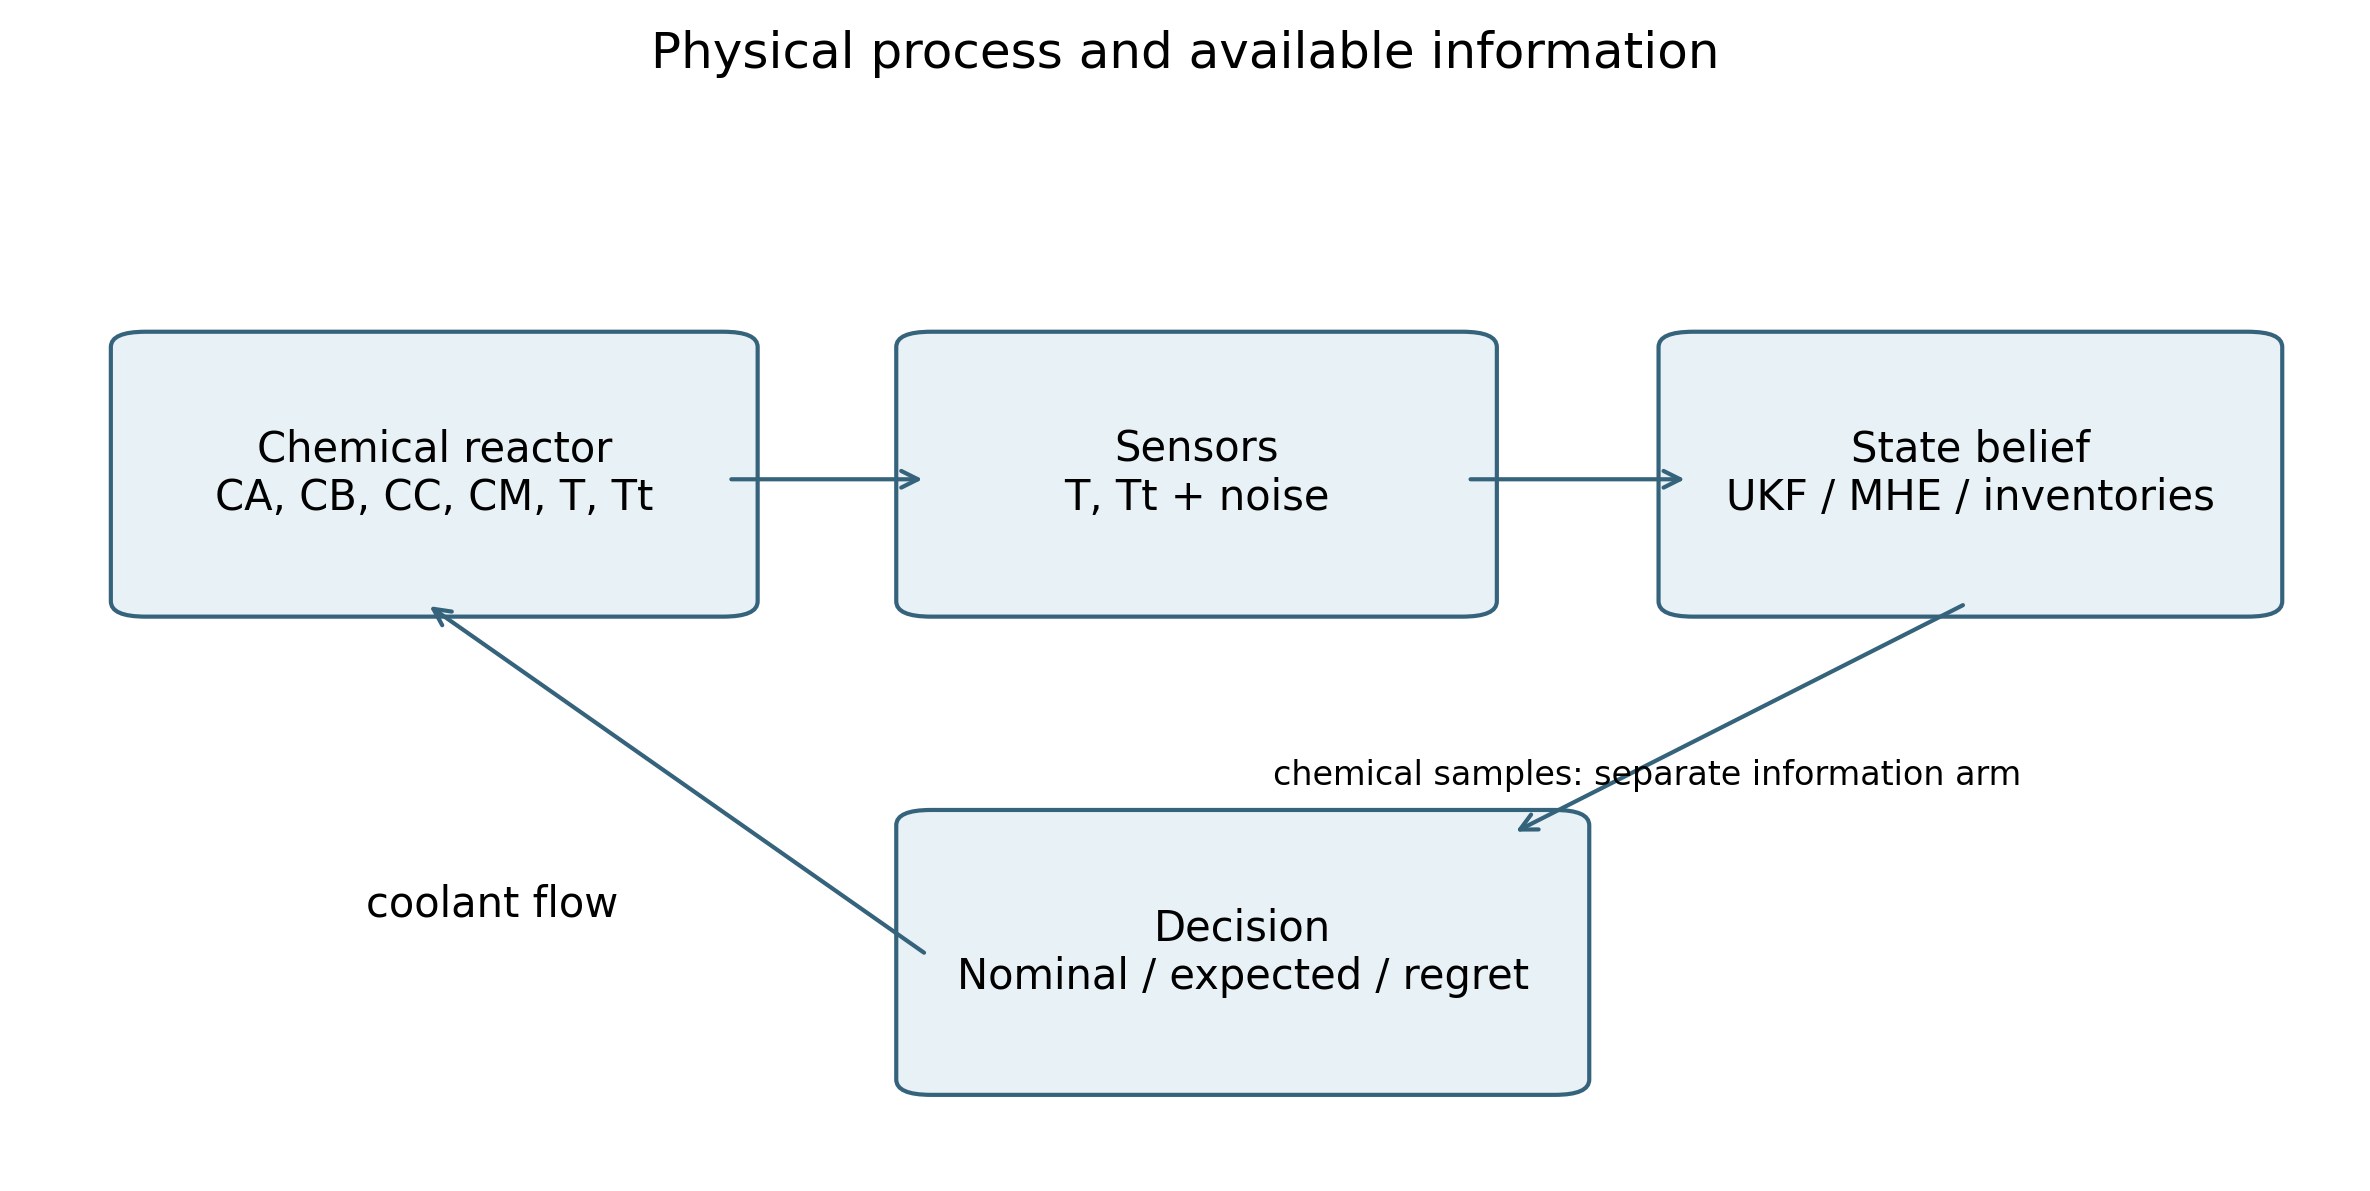
\includegraphics{figures/Figure_01.png}
\caption{Figure 1. Physical process and available information}
\end{figure}

\begin{figure}
\centering
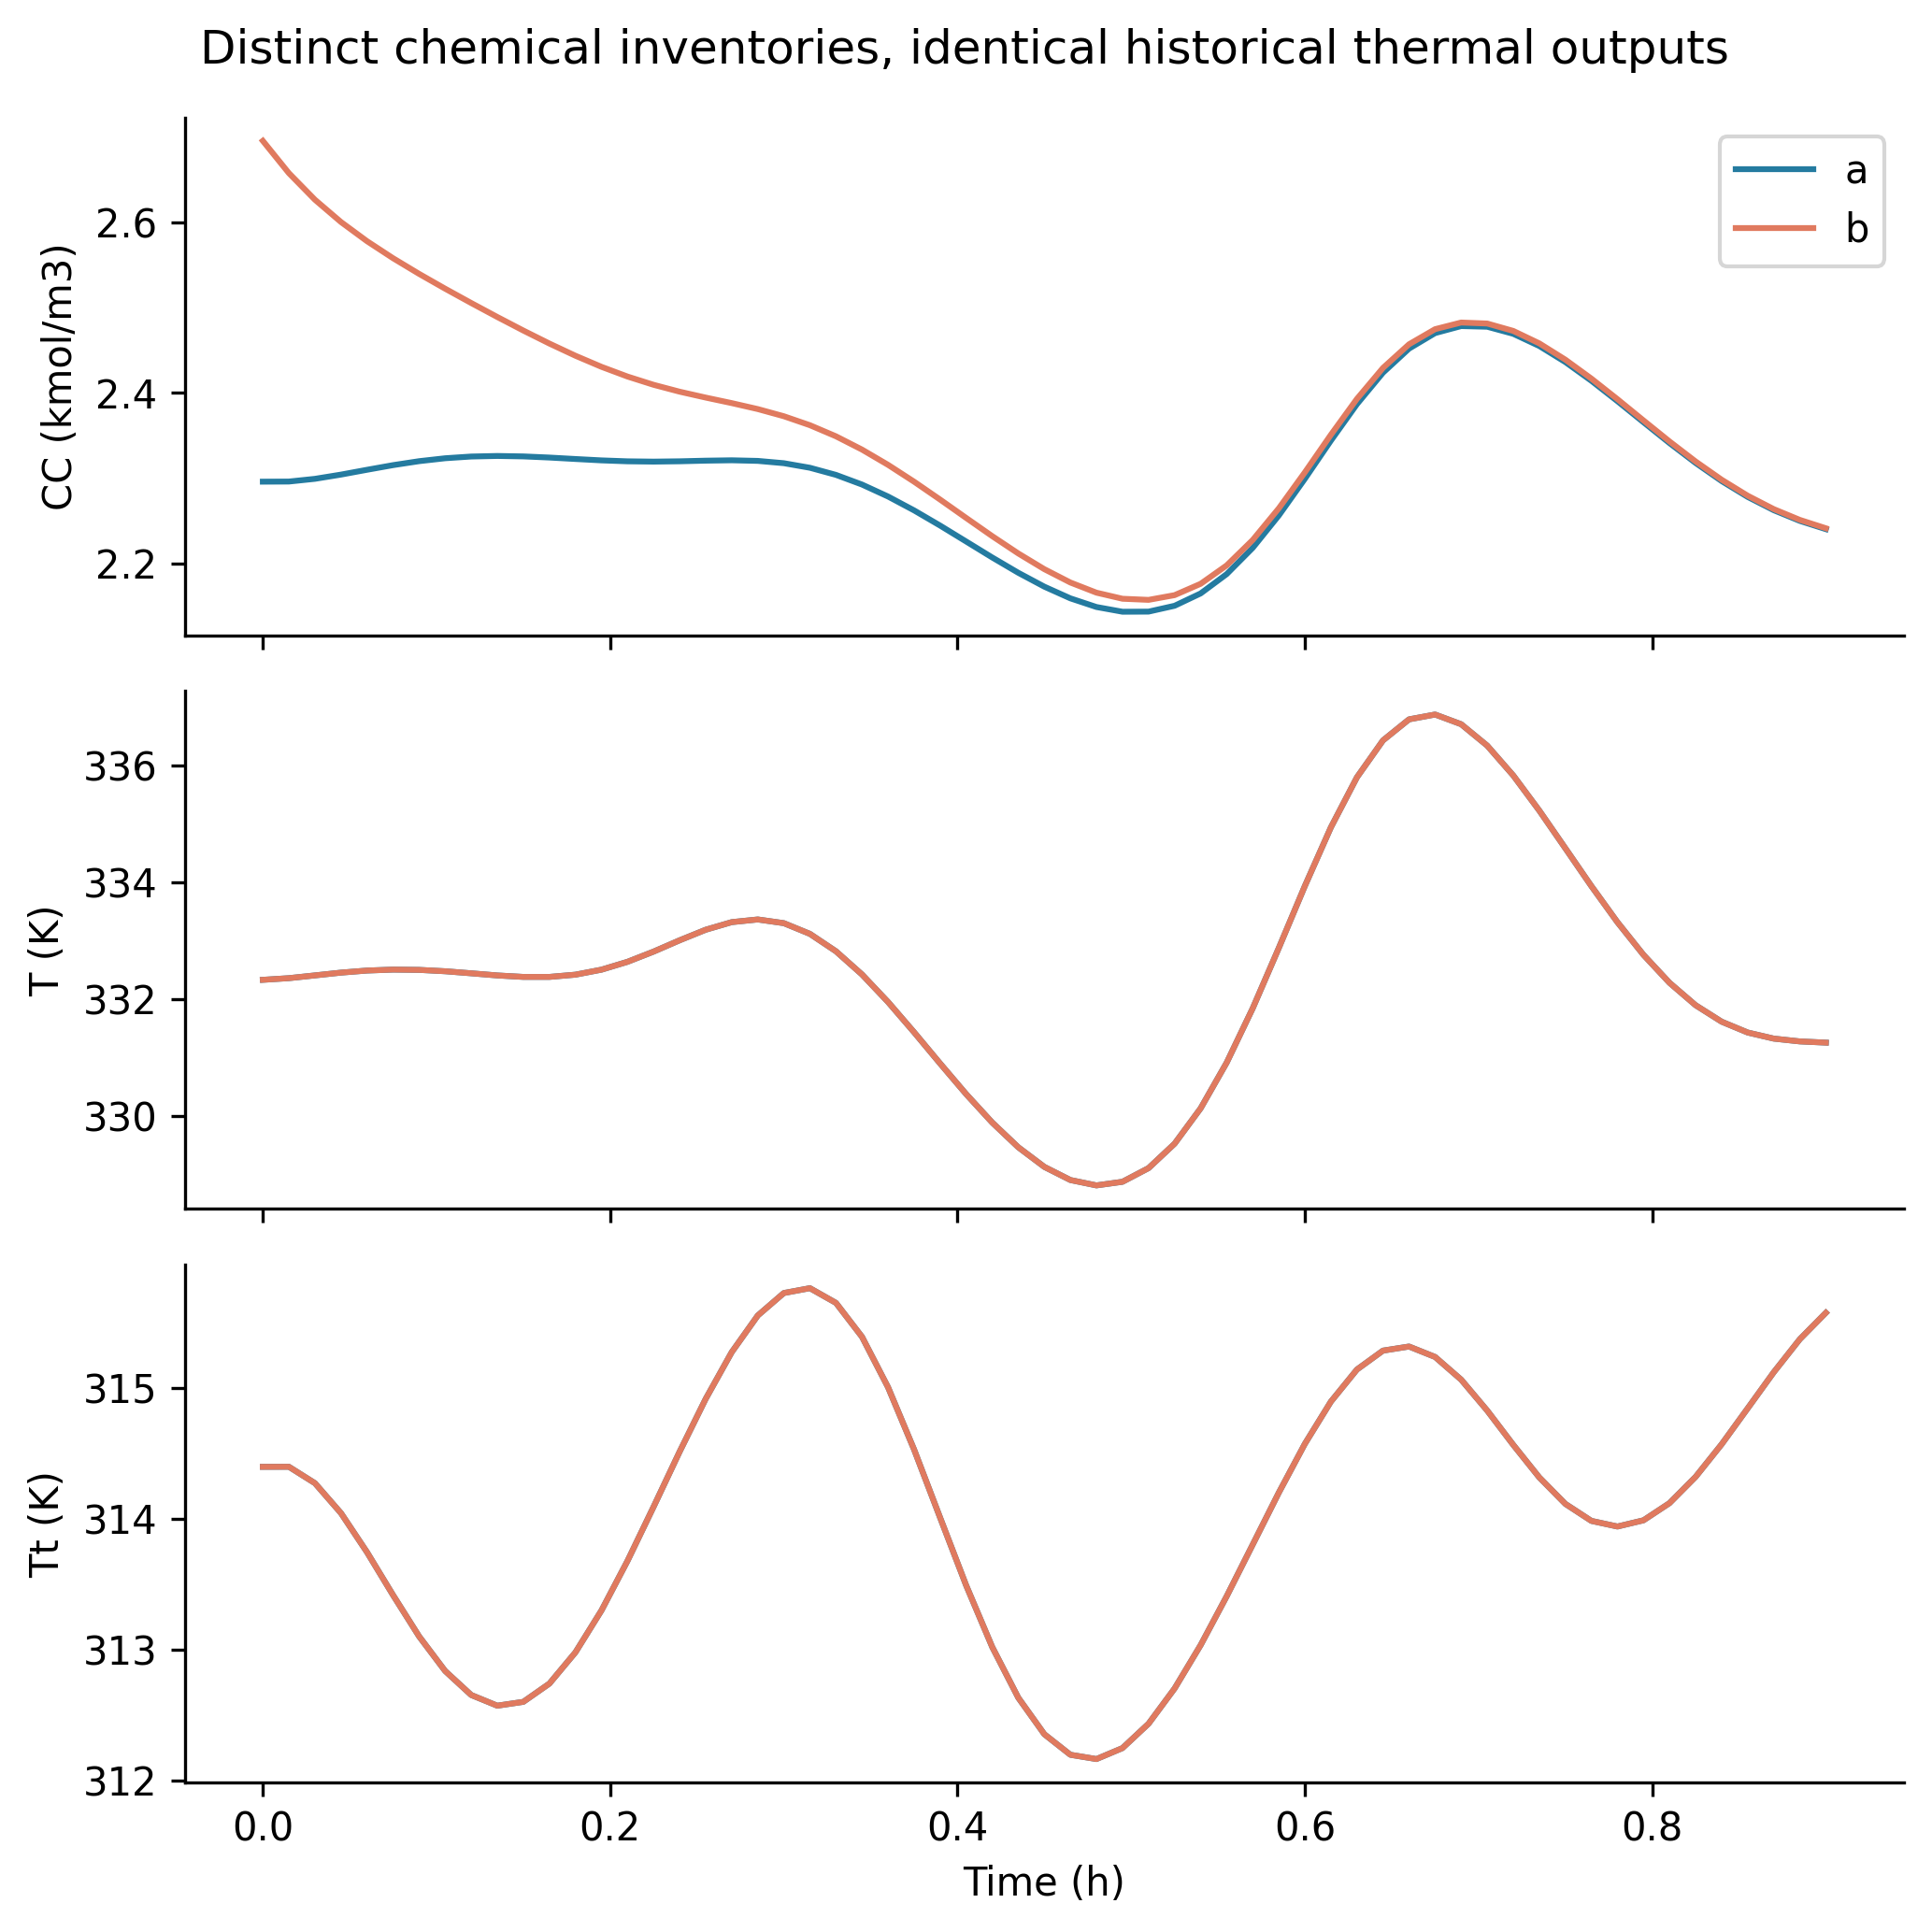
\includegraphics{figures/Figure_02.png}
\caption{Figure 2. Distinct chemical inventories, identical historical
thermal outputs}
\end{figure}

\begin{figure}
\centering
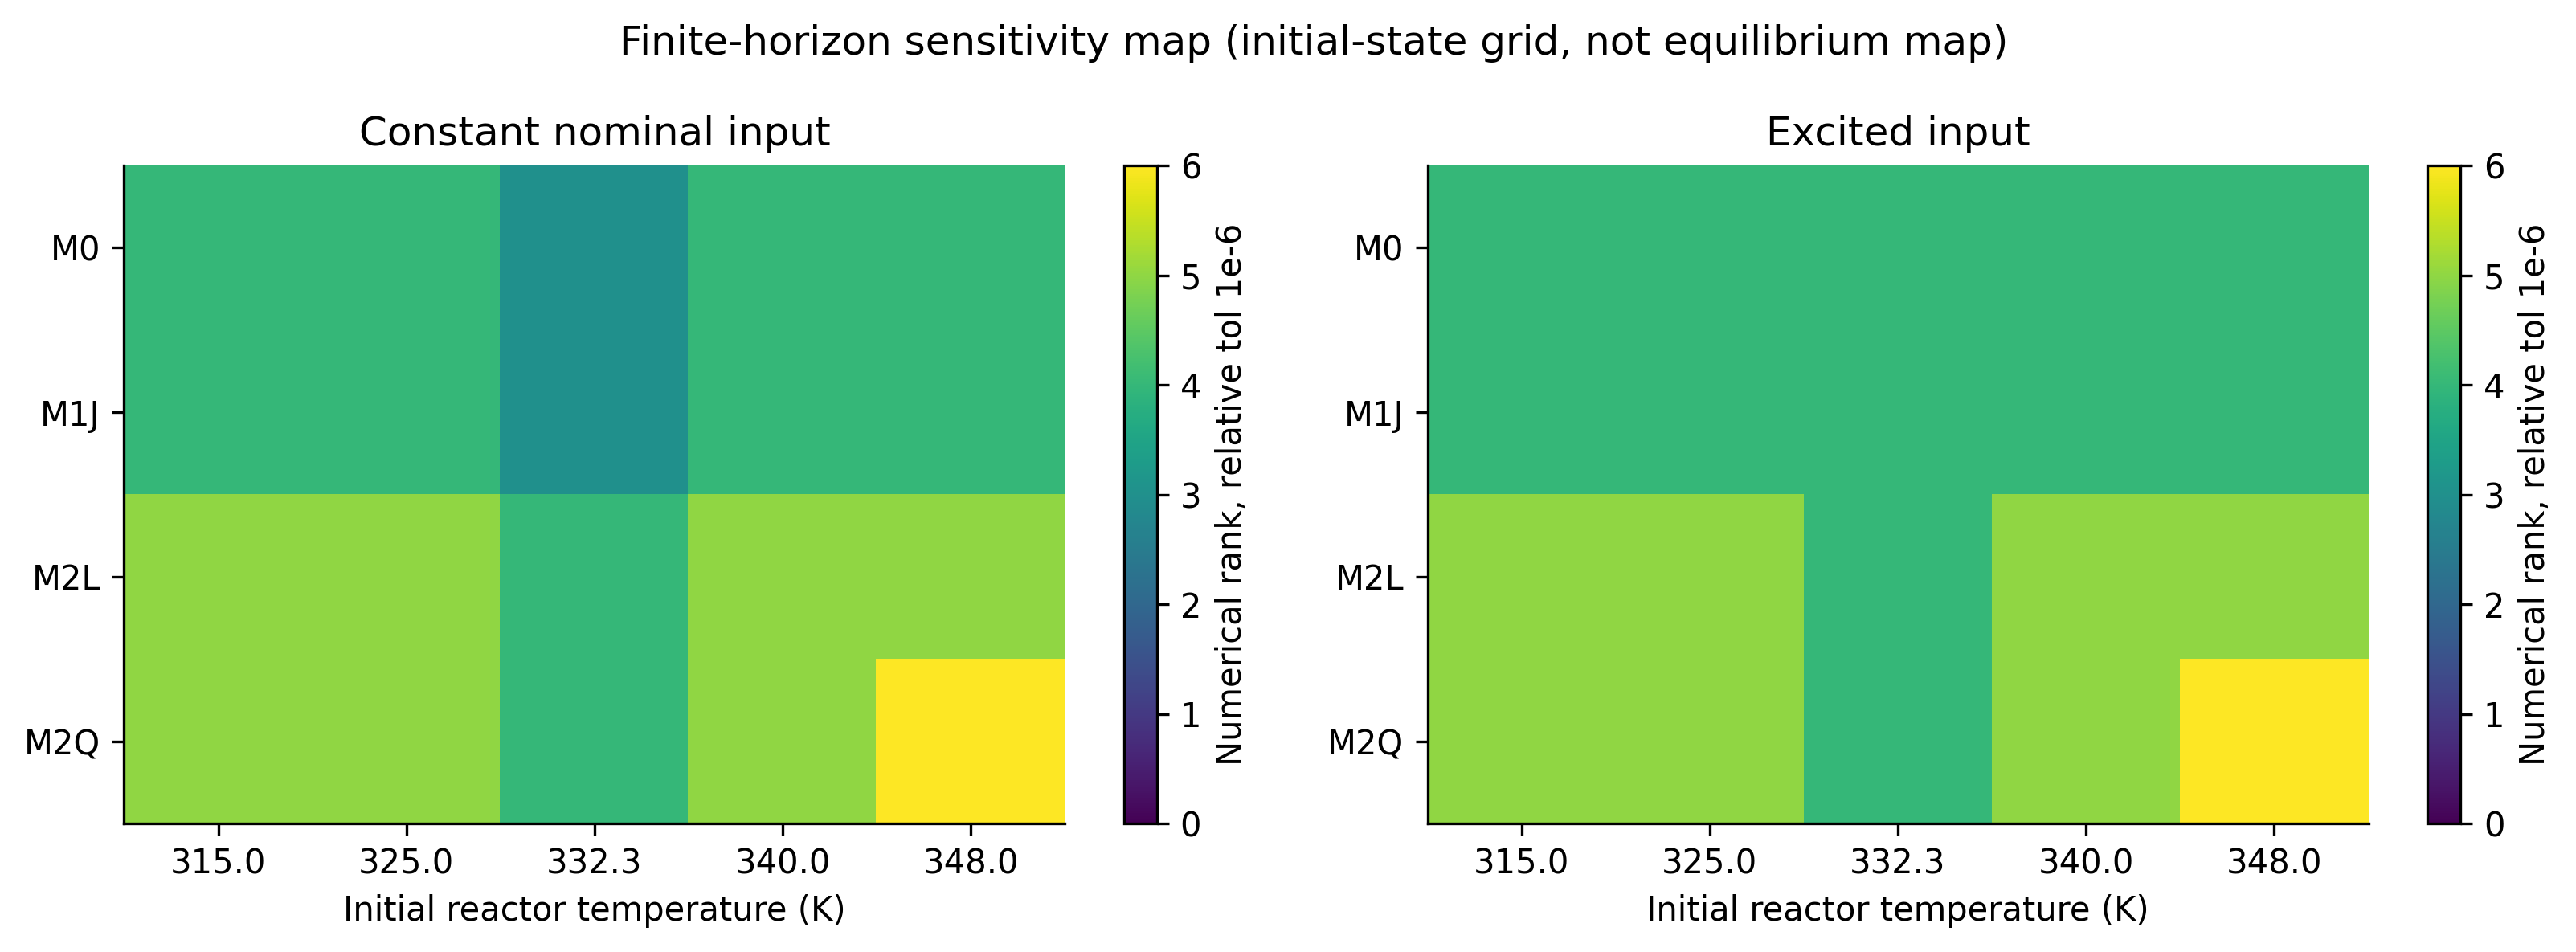
\includegraphics{figures/Figure_03.png}
\caption{Figure 3. Finite-horizon sensitivity map (initial-state grid,
not equilibrium map)}
\end{figure}

\begin{figure}
\centering
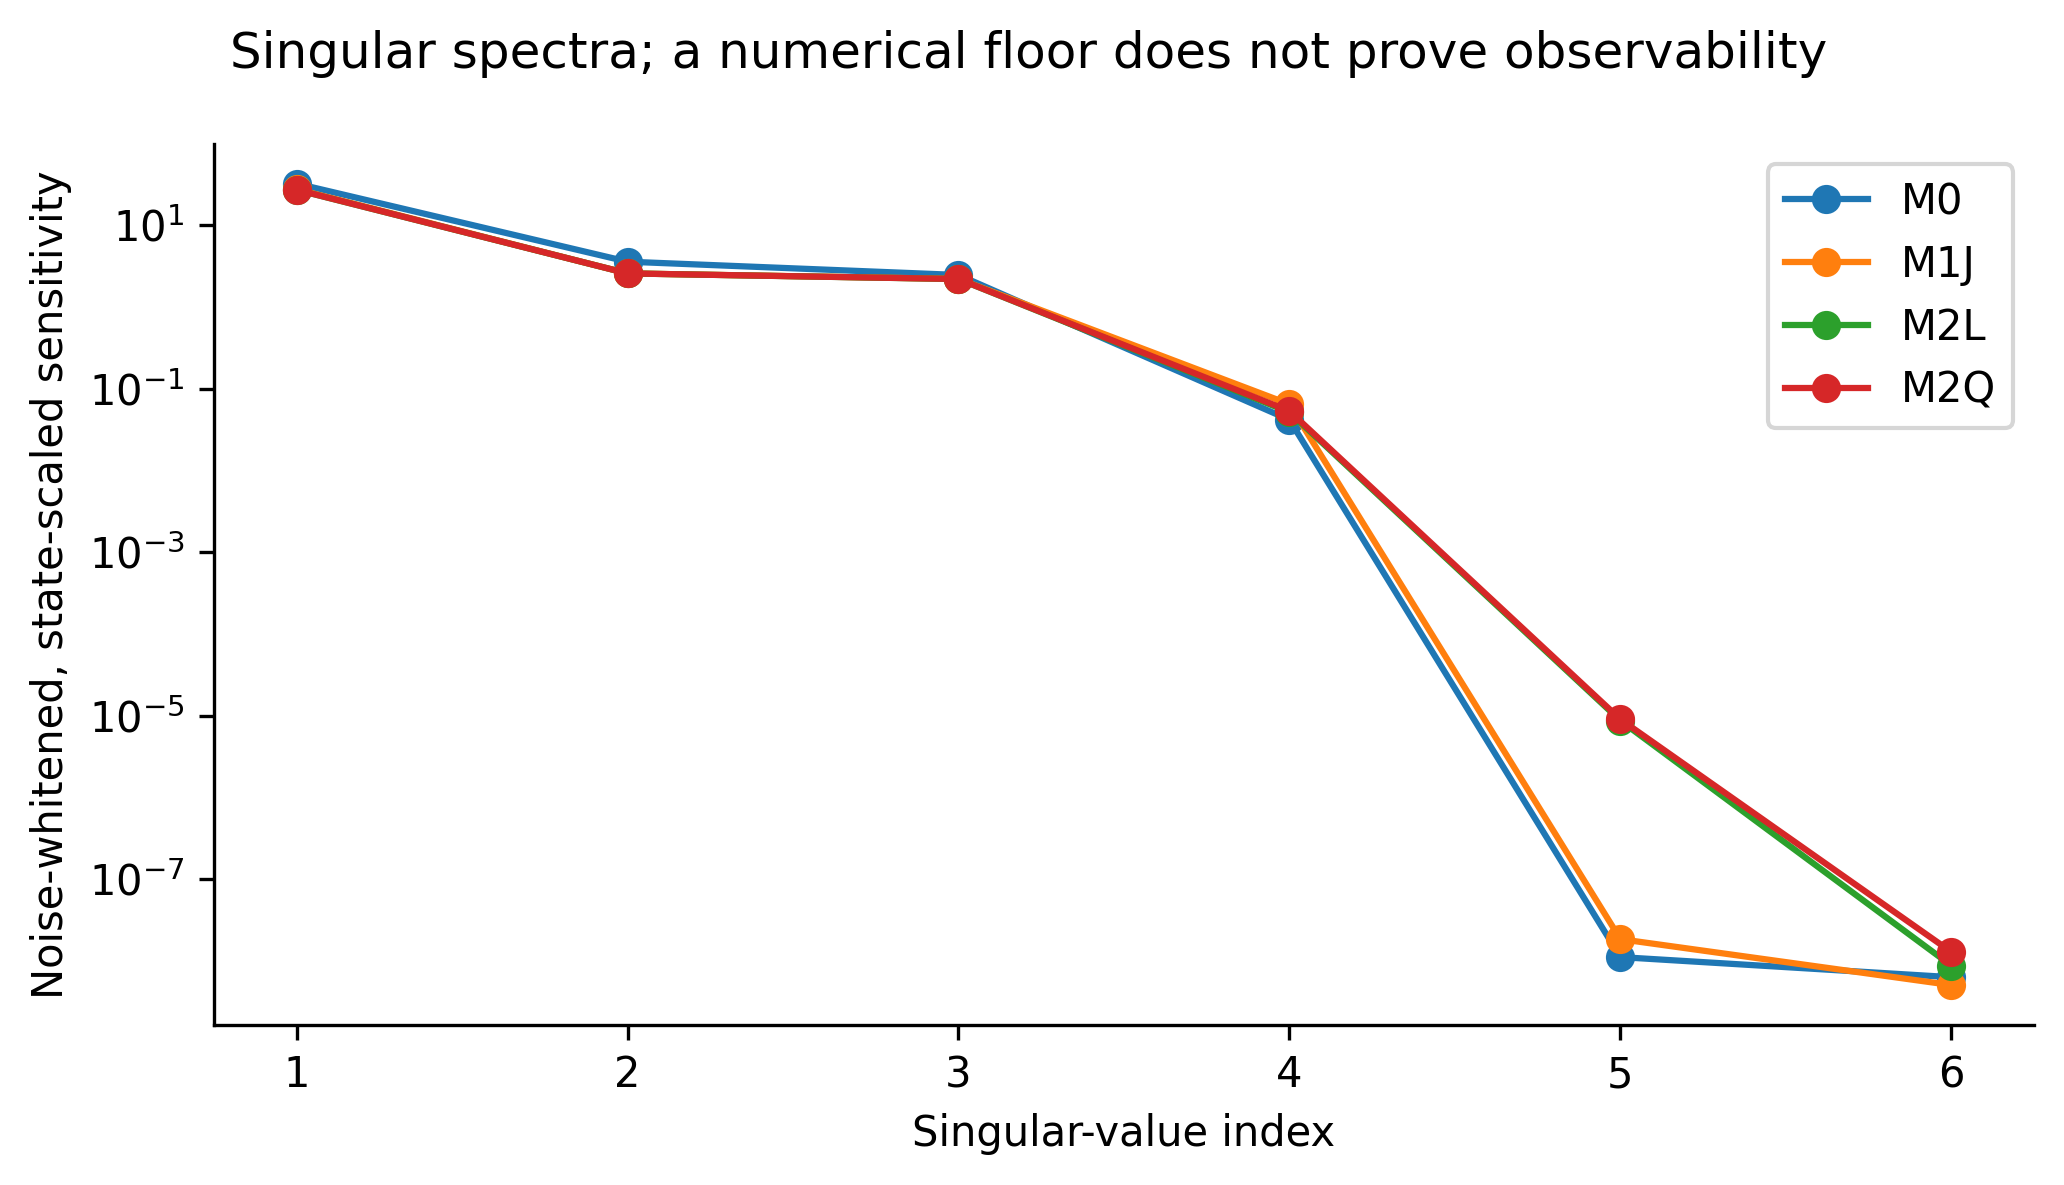
\includegraphics{figures/Figure_04.png}
\caption{Figure 4. Singular spectra; a numerical floor does not prove
observability}
\end{figure}

\begin{figure}
\centering
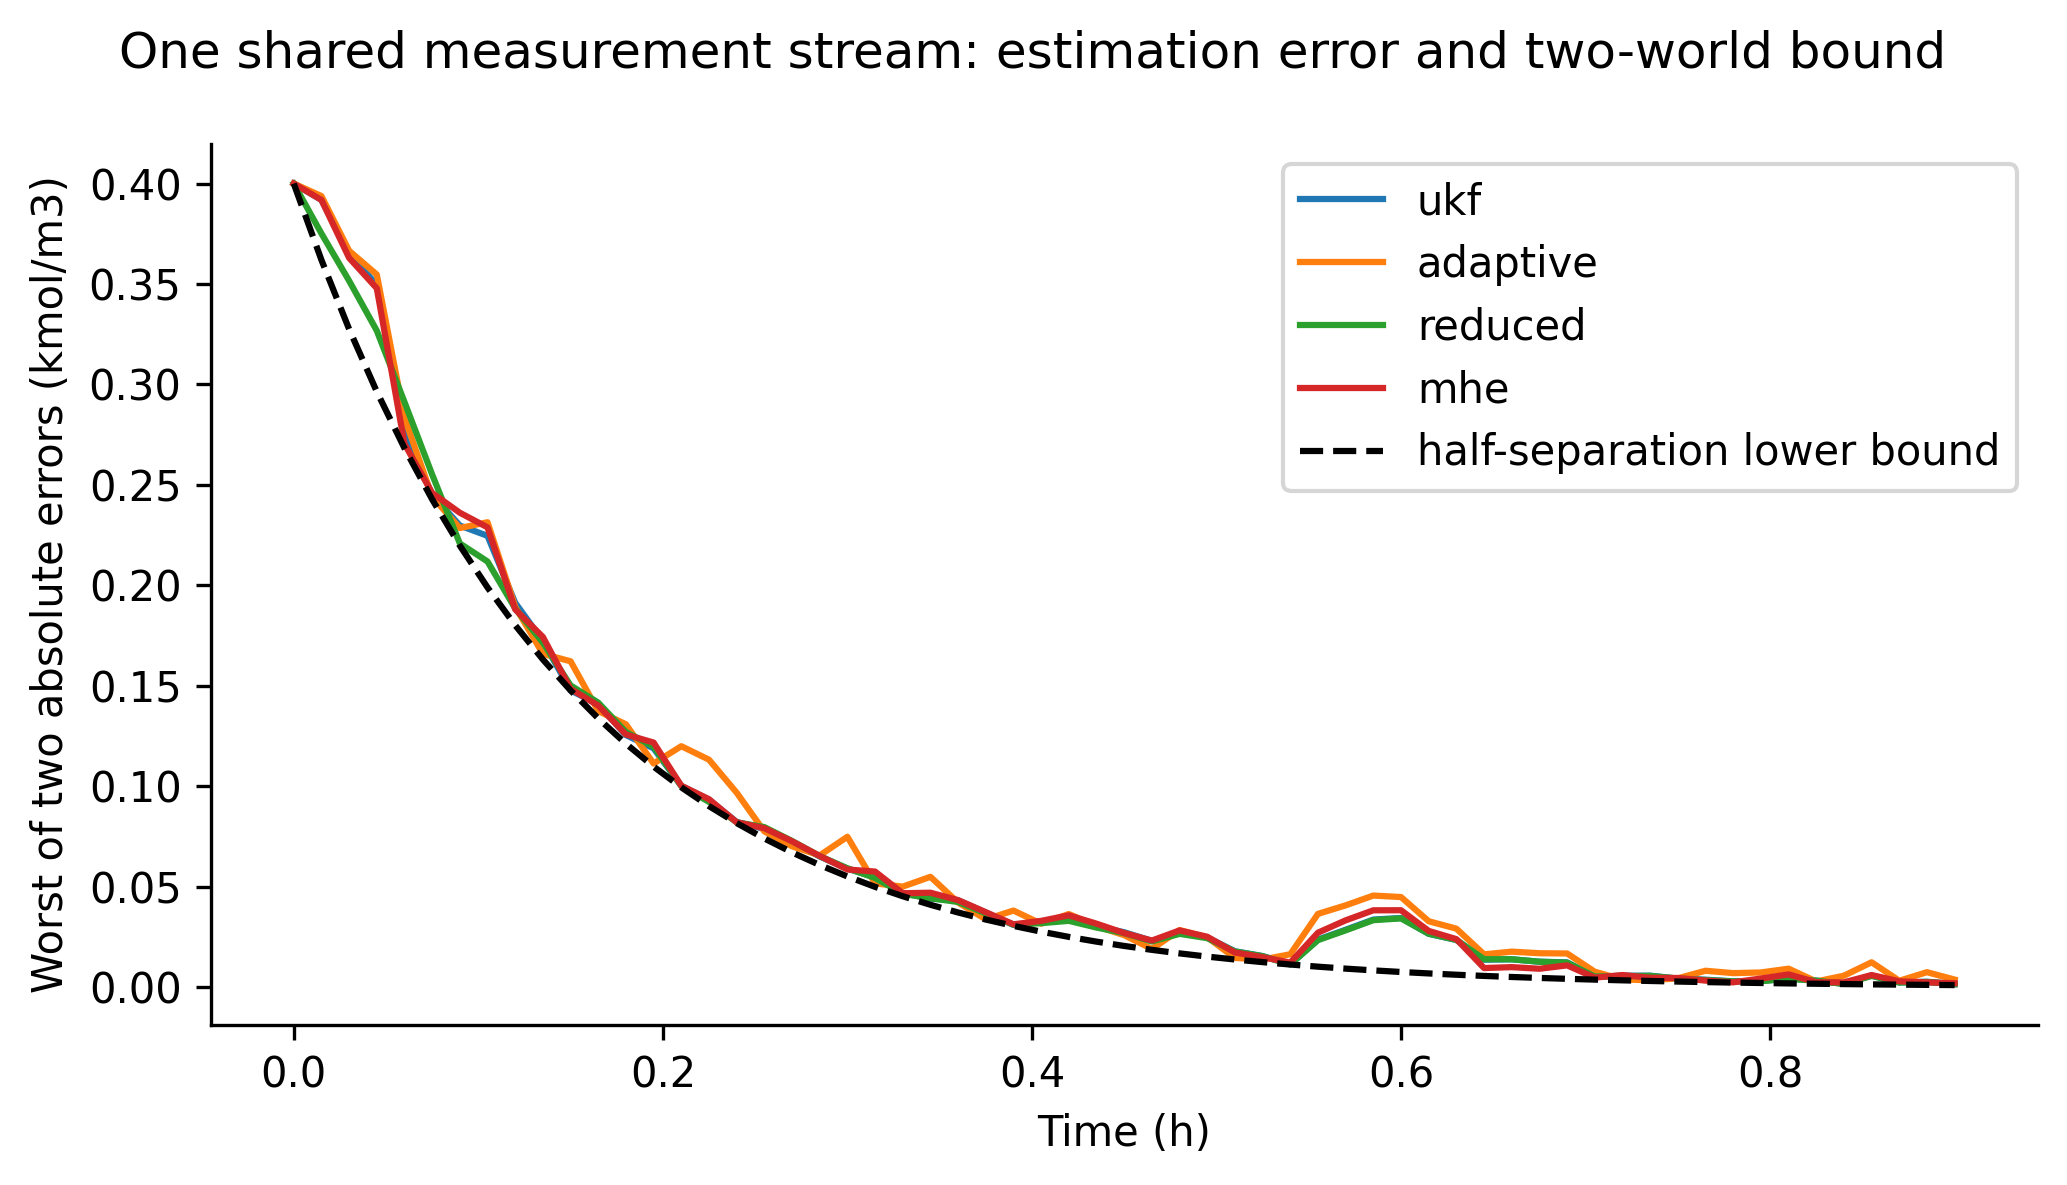
\includegraphics{figures/Figure_05.png}
\caption{Figure 5. One shared measurement stream: estimation error and
two-world bound}
\end{figure}

\begin{figure}
\centering
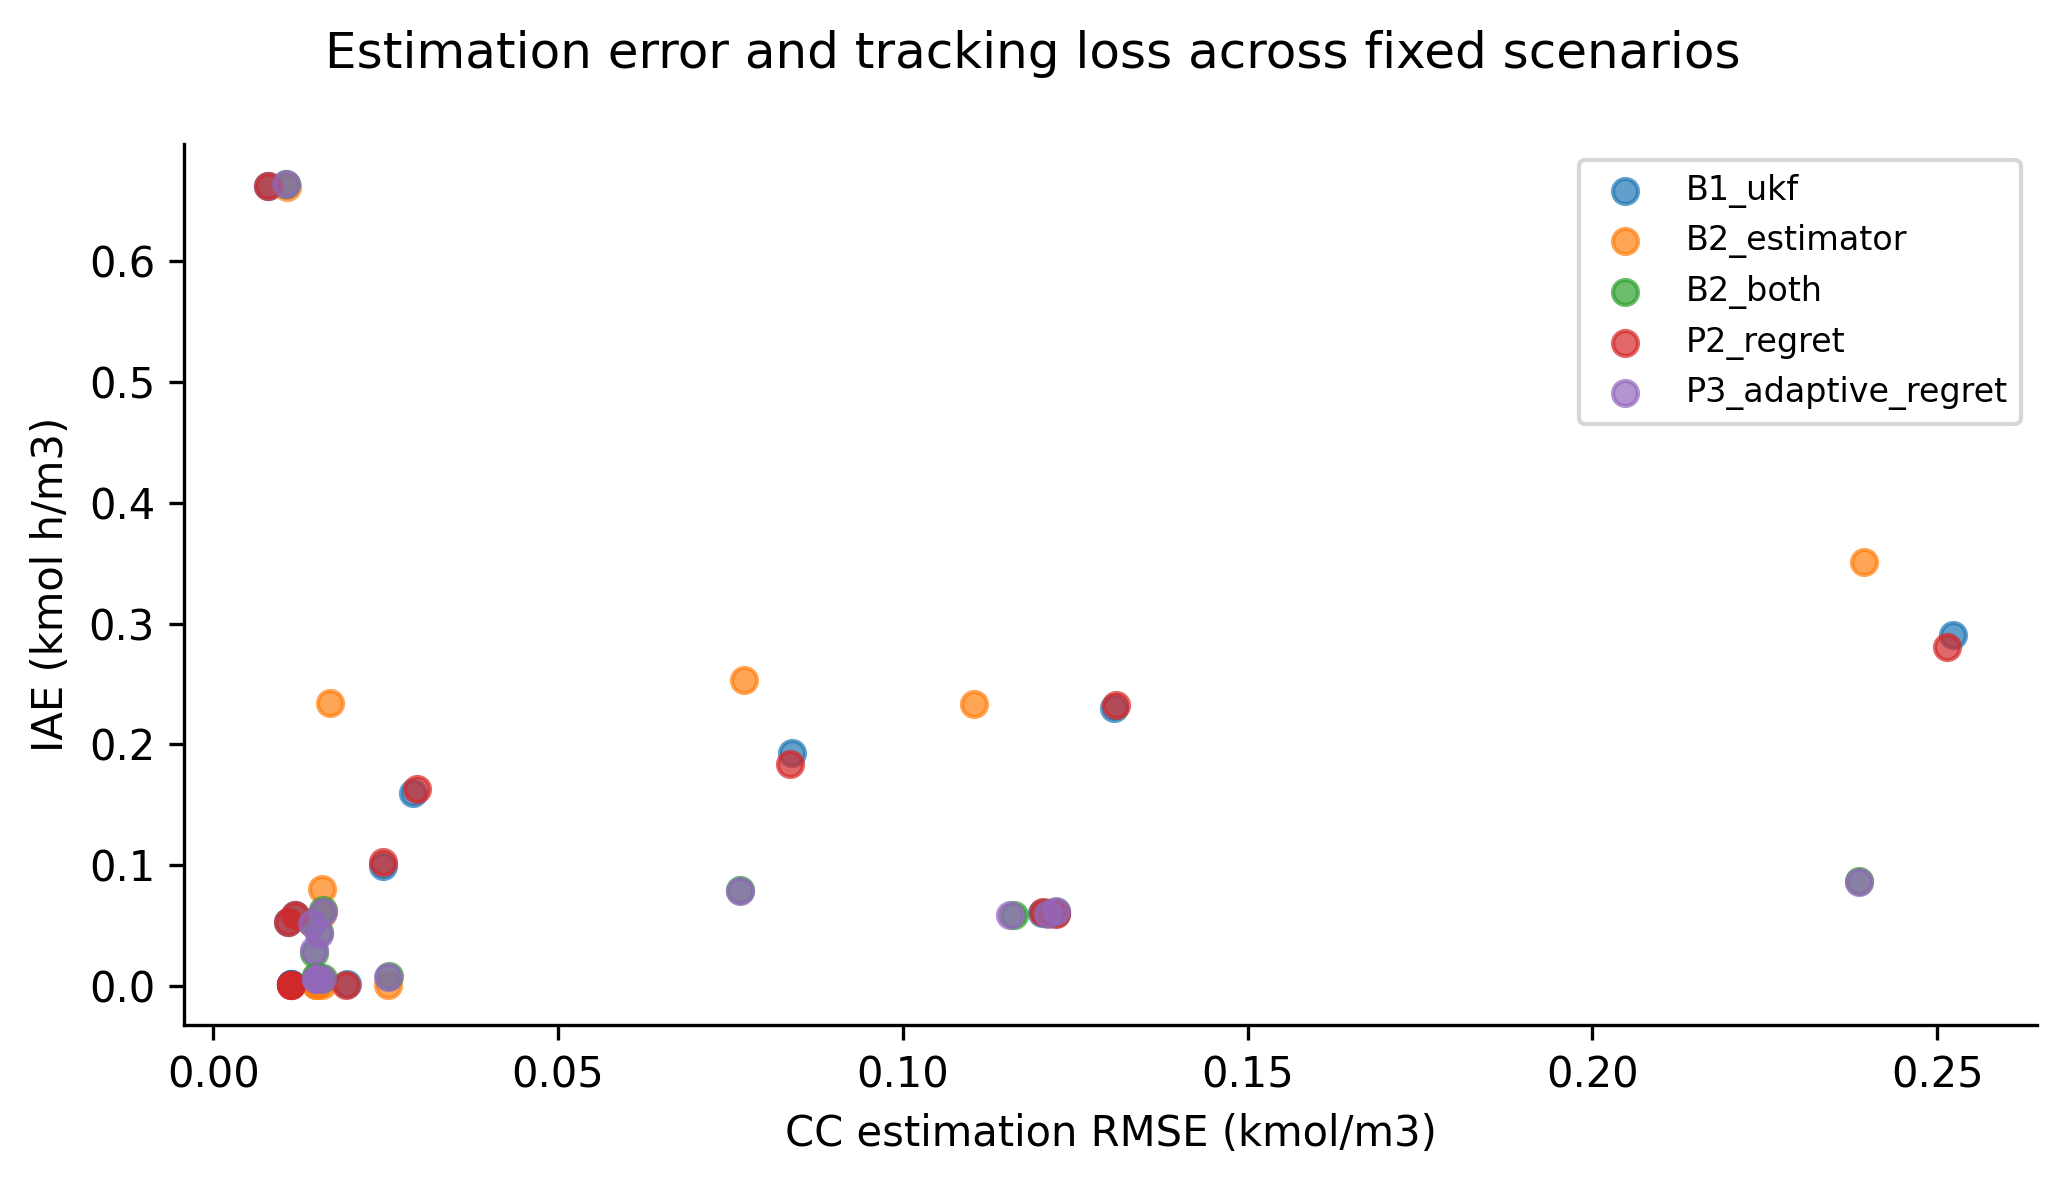
\includegraphics{figures/Figure_06.png}
\caption{Figure 6. Estimation error and tracking loss across fixed
scenarios}
\end{figure}

\begin{figure}
\centering
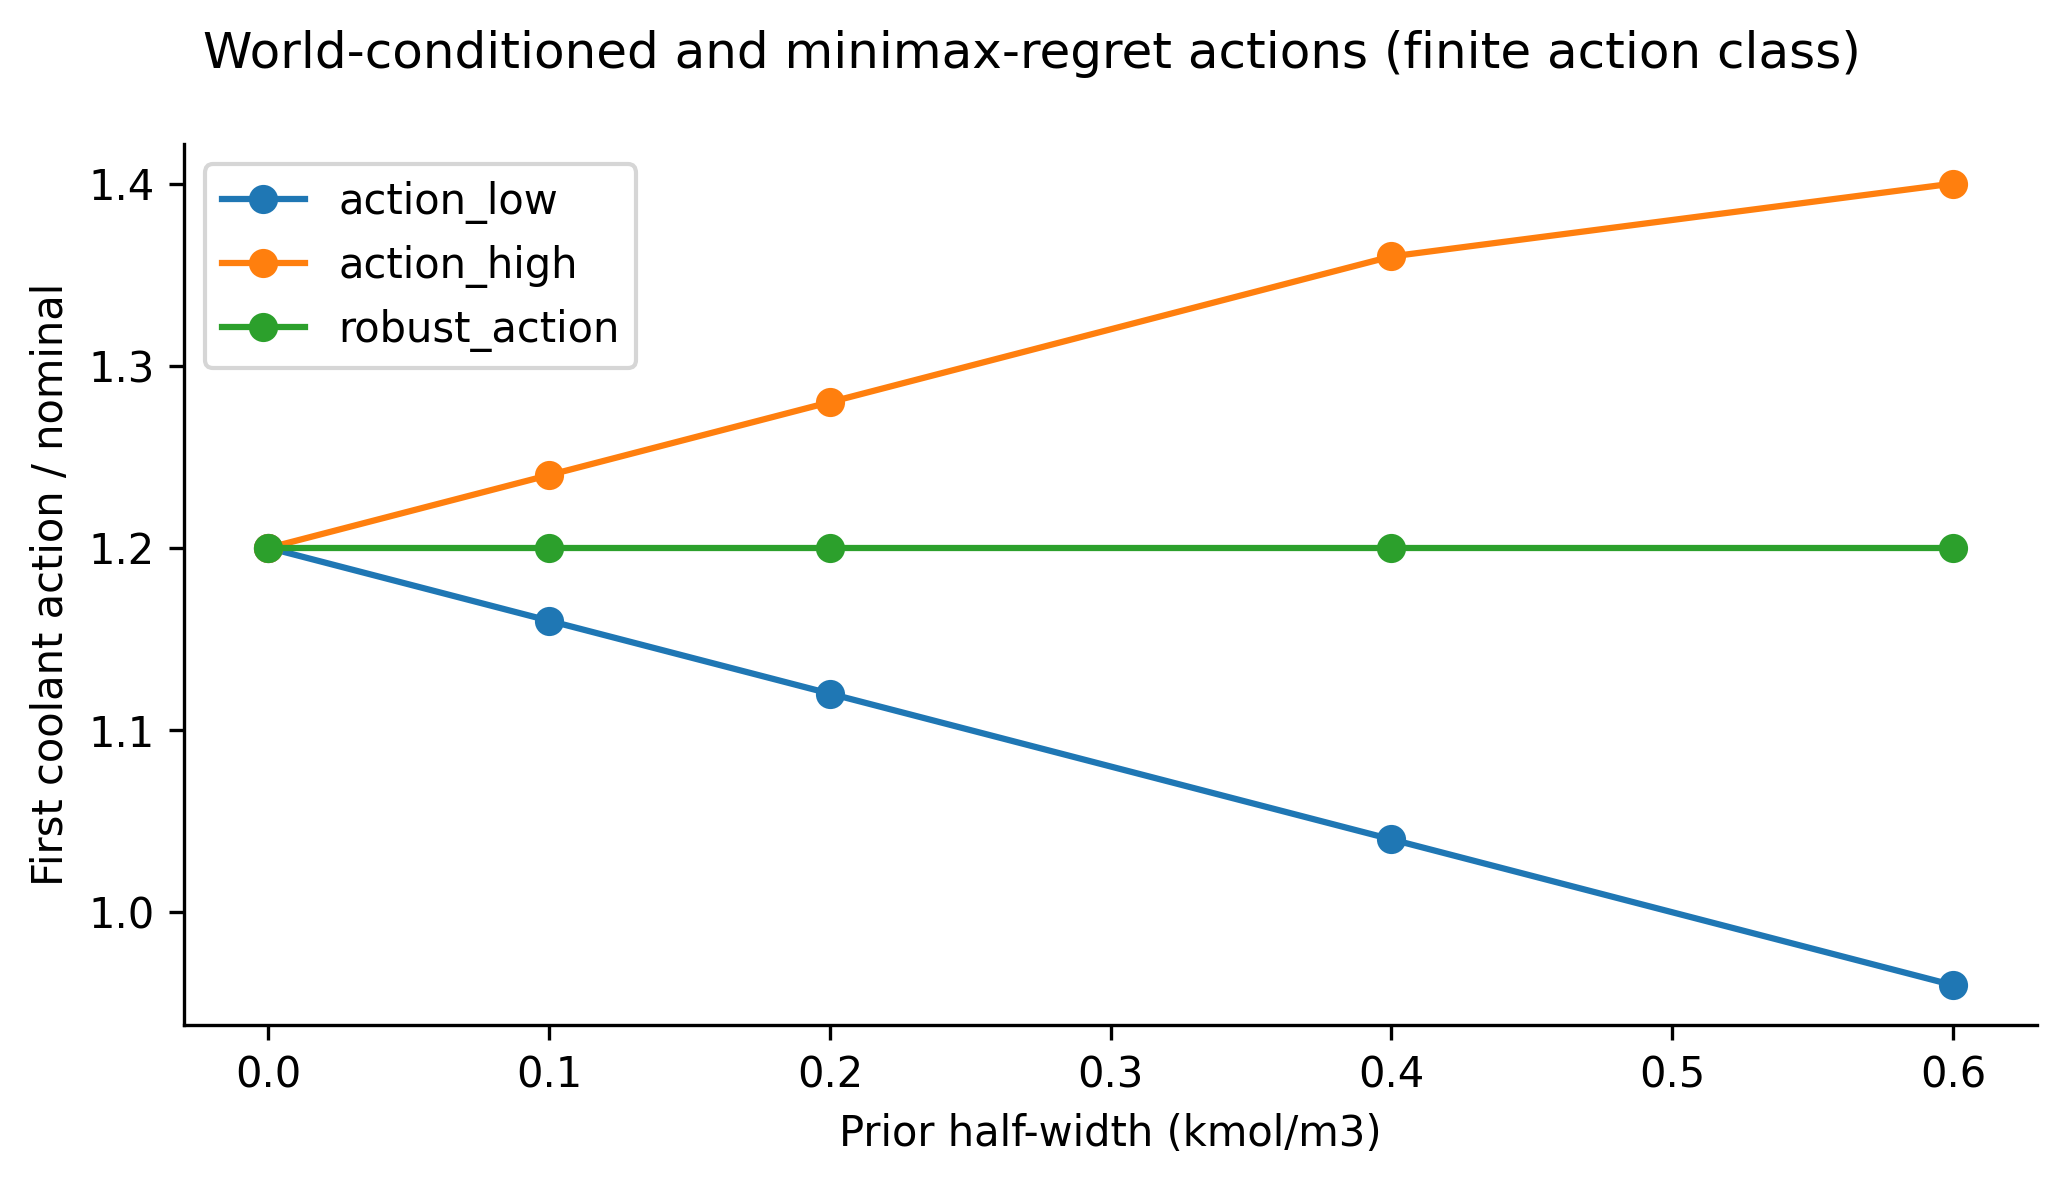
\includegraphics{figures/Figure_07.png}
\caption{Figure 7. World-conditioned and minimax-regret actions (finite
action class)}
\end{figure}

\begin{figure}
\centering
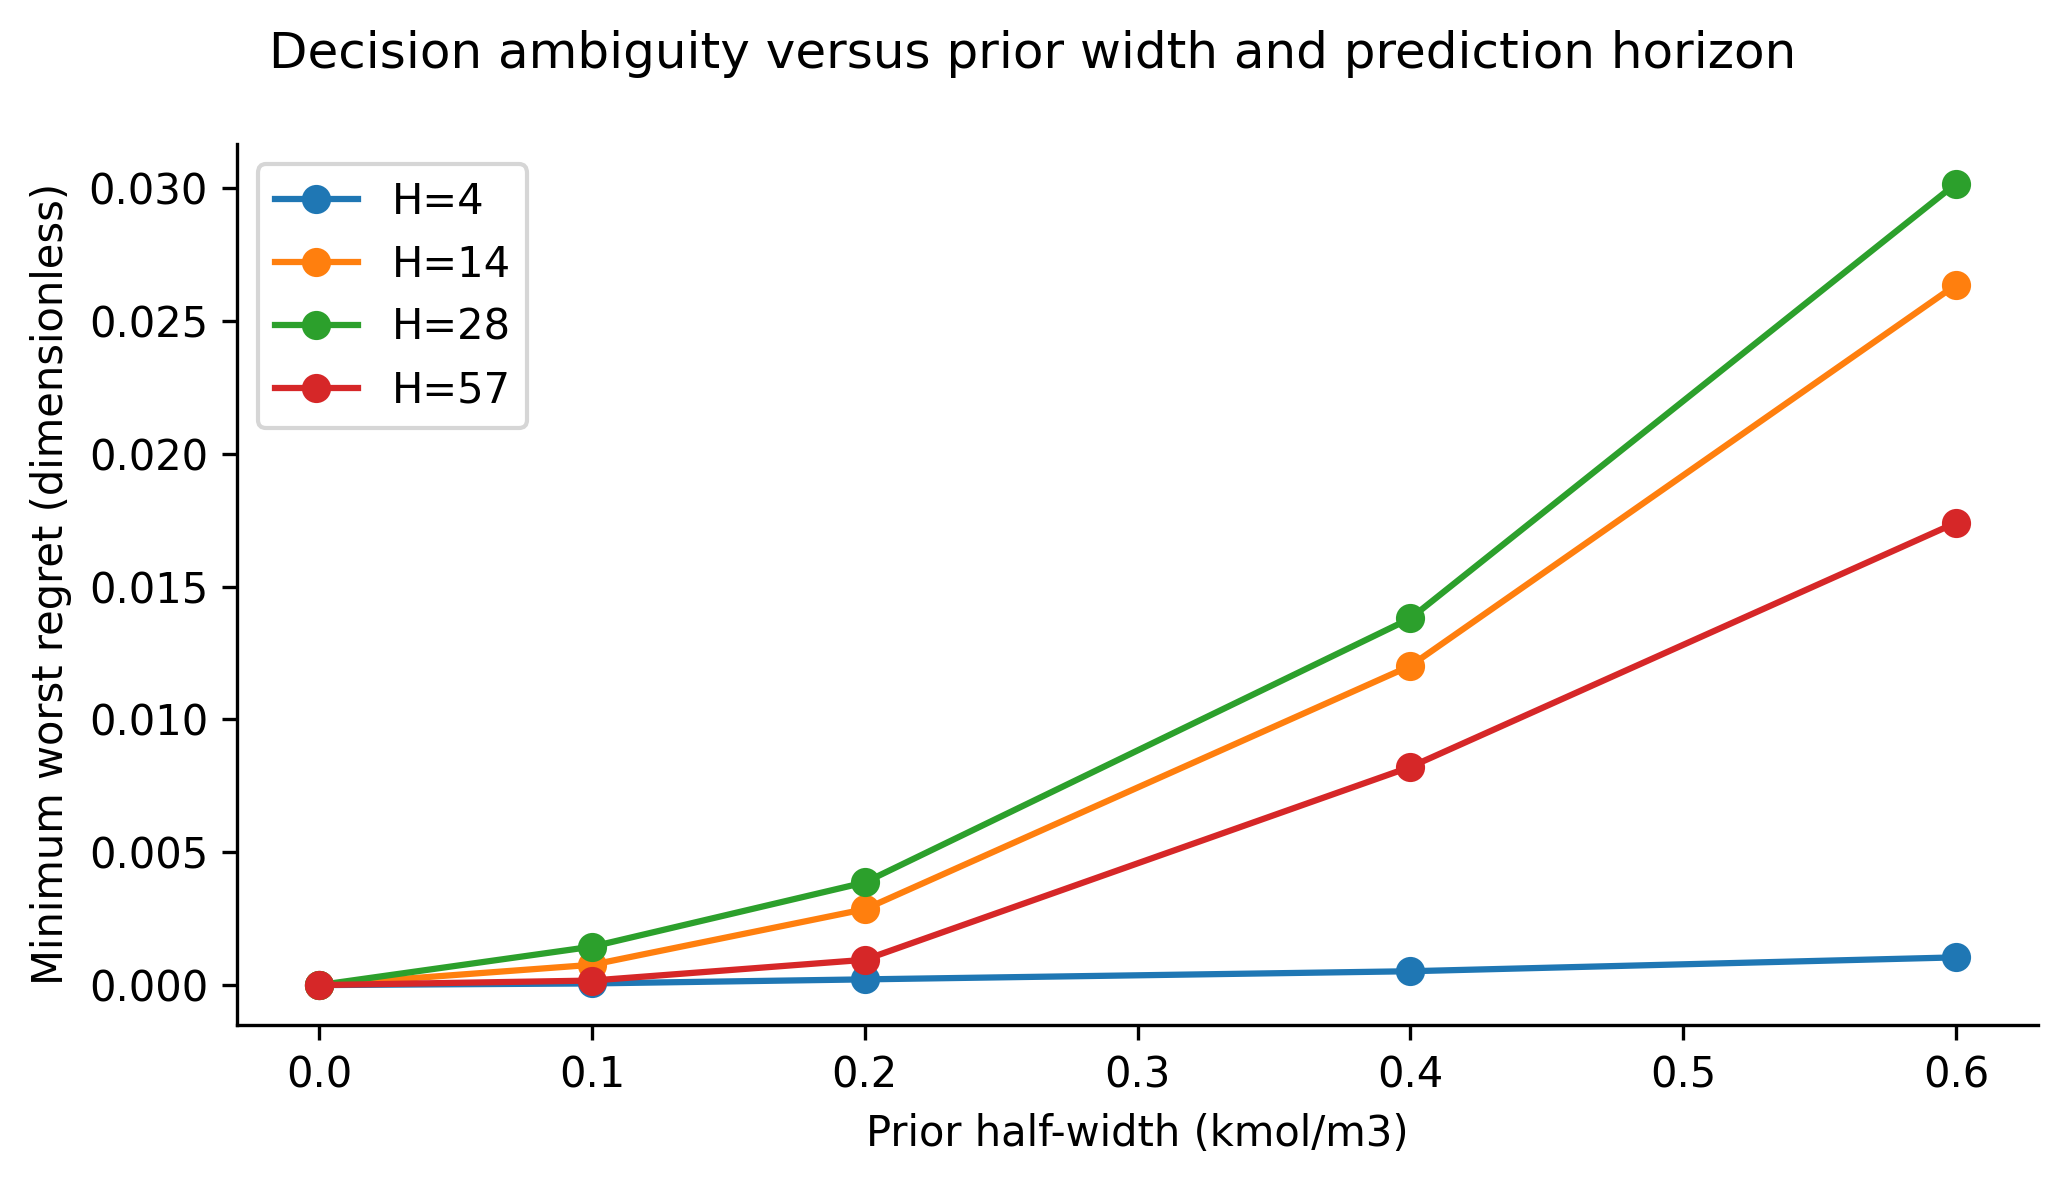
\includegraphics{figures/Figure_08.png}
\caption{Figure 8. Decision ambiguity versus prior width and prediction
horizon}
\end{figure}

\begin{figure}
\centering
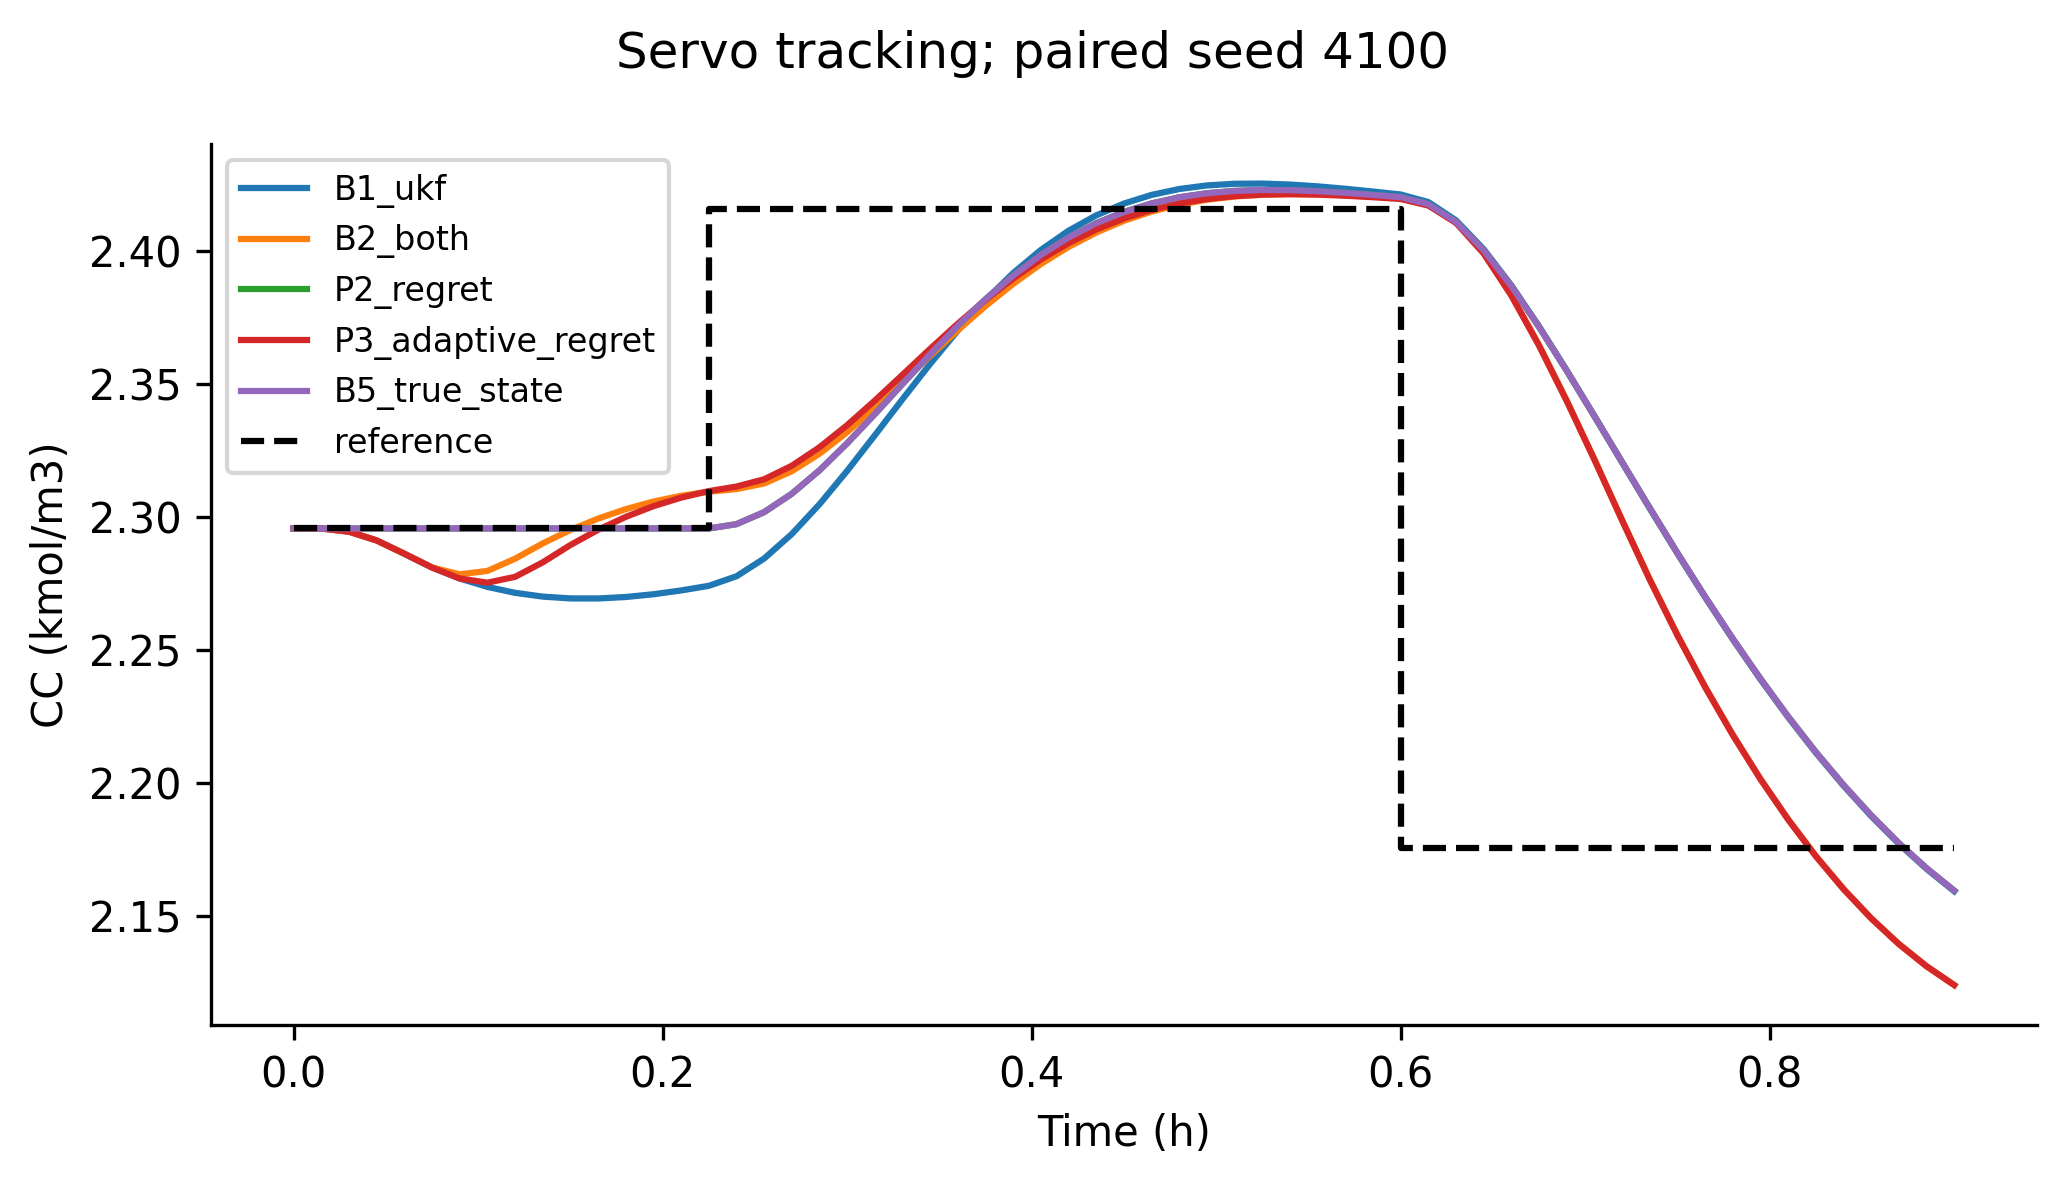
\includegraphics{figures/Figure_09.png}
\caption{Figure 9. Servo tracking; paired seed 4100}
\end{figure}

\begin{figure}
\centering
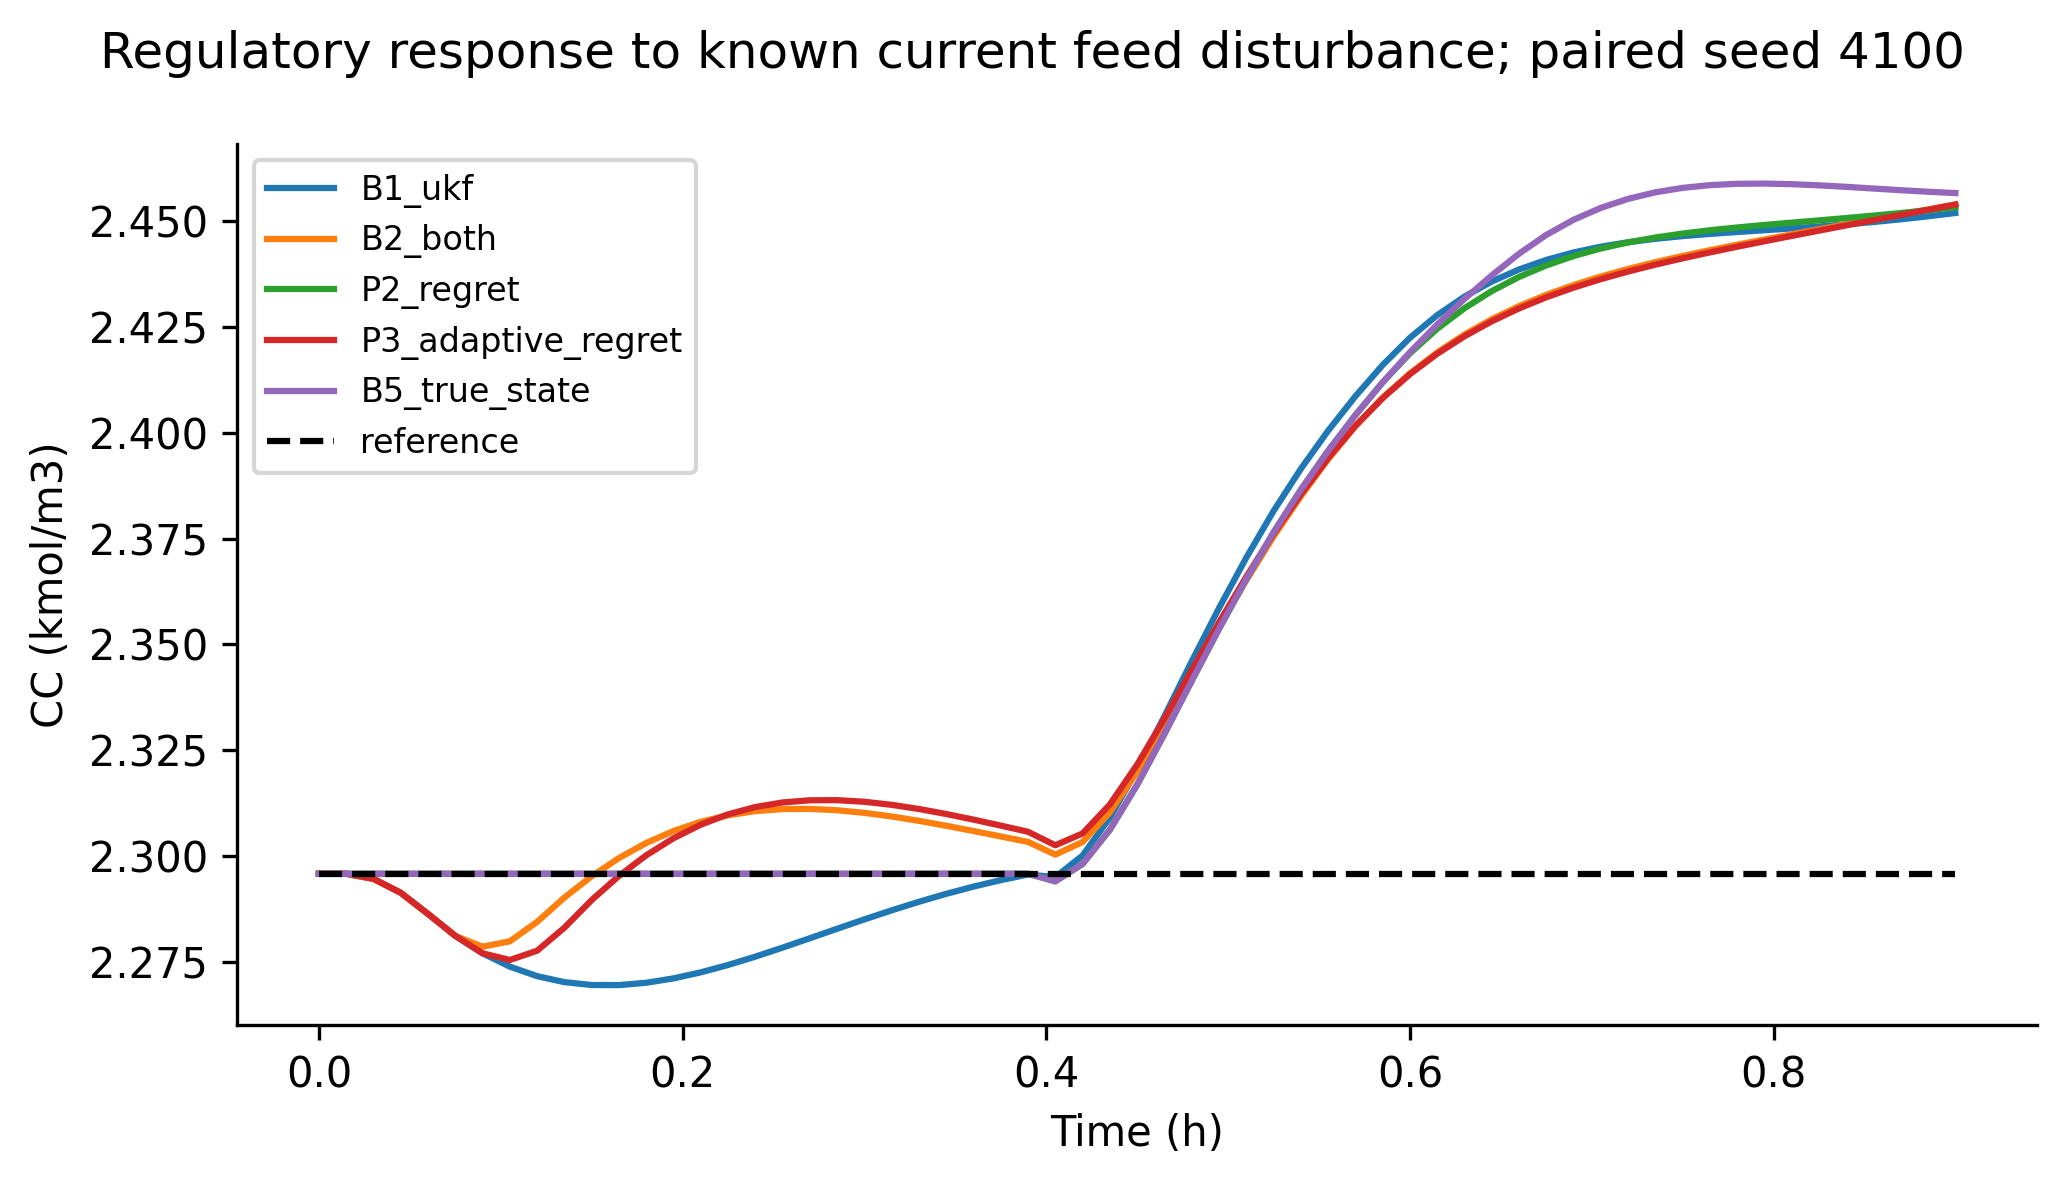
\includegraphics{figures/Figure_10.png}
\caption{Figure 10. Regulatory response to known current feed
disturbance; paired seed 4100}
\end{figure}

\begin{figure}
\centering
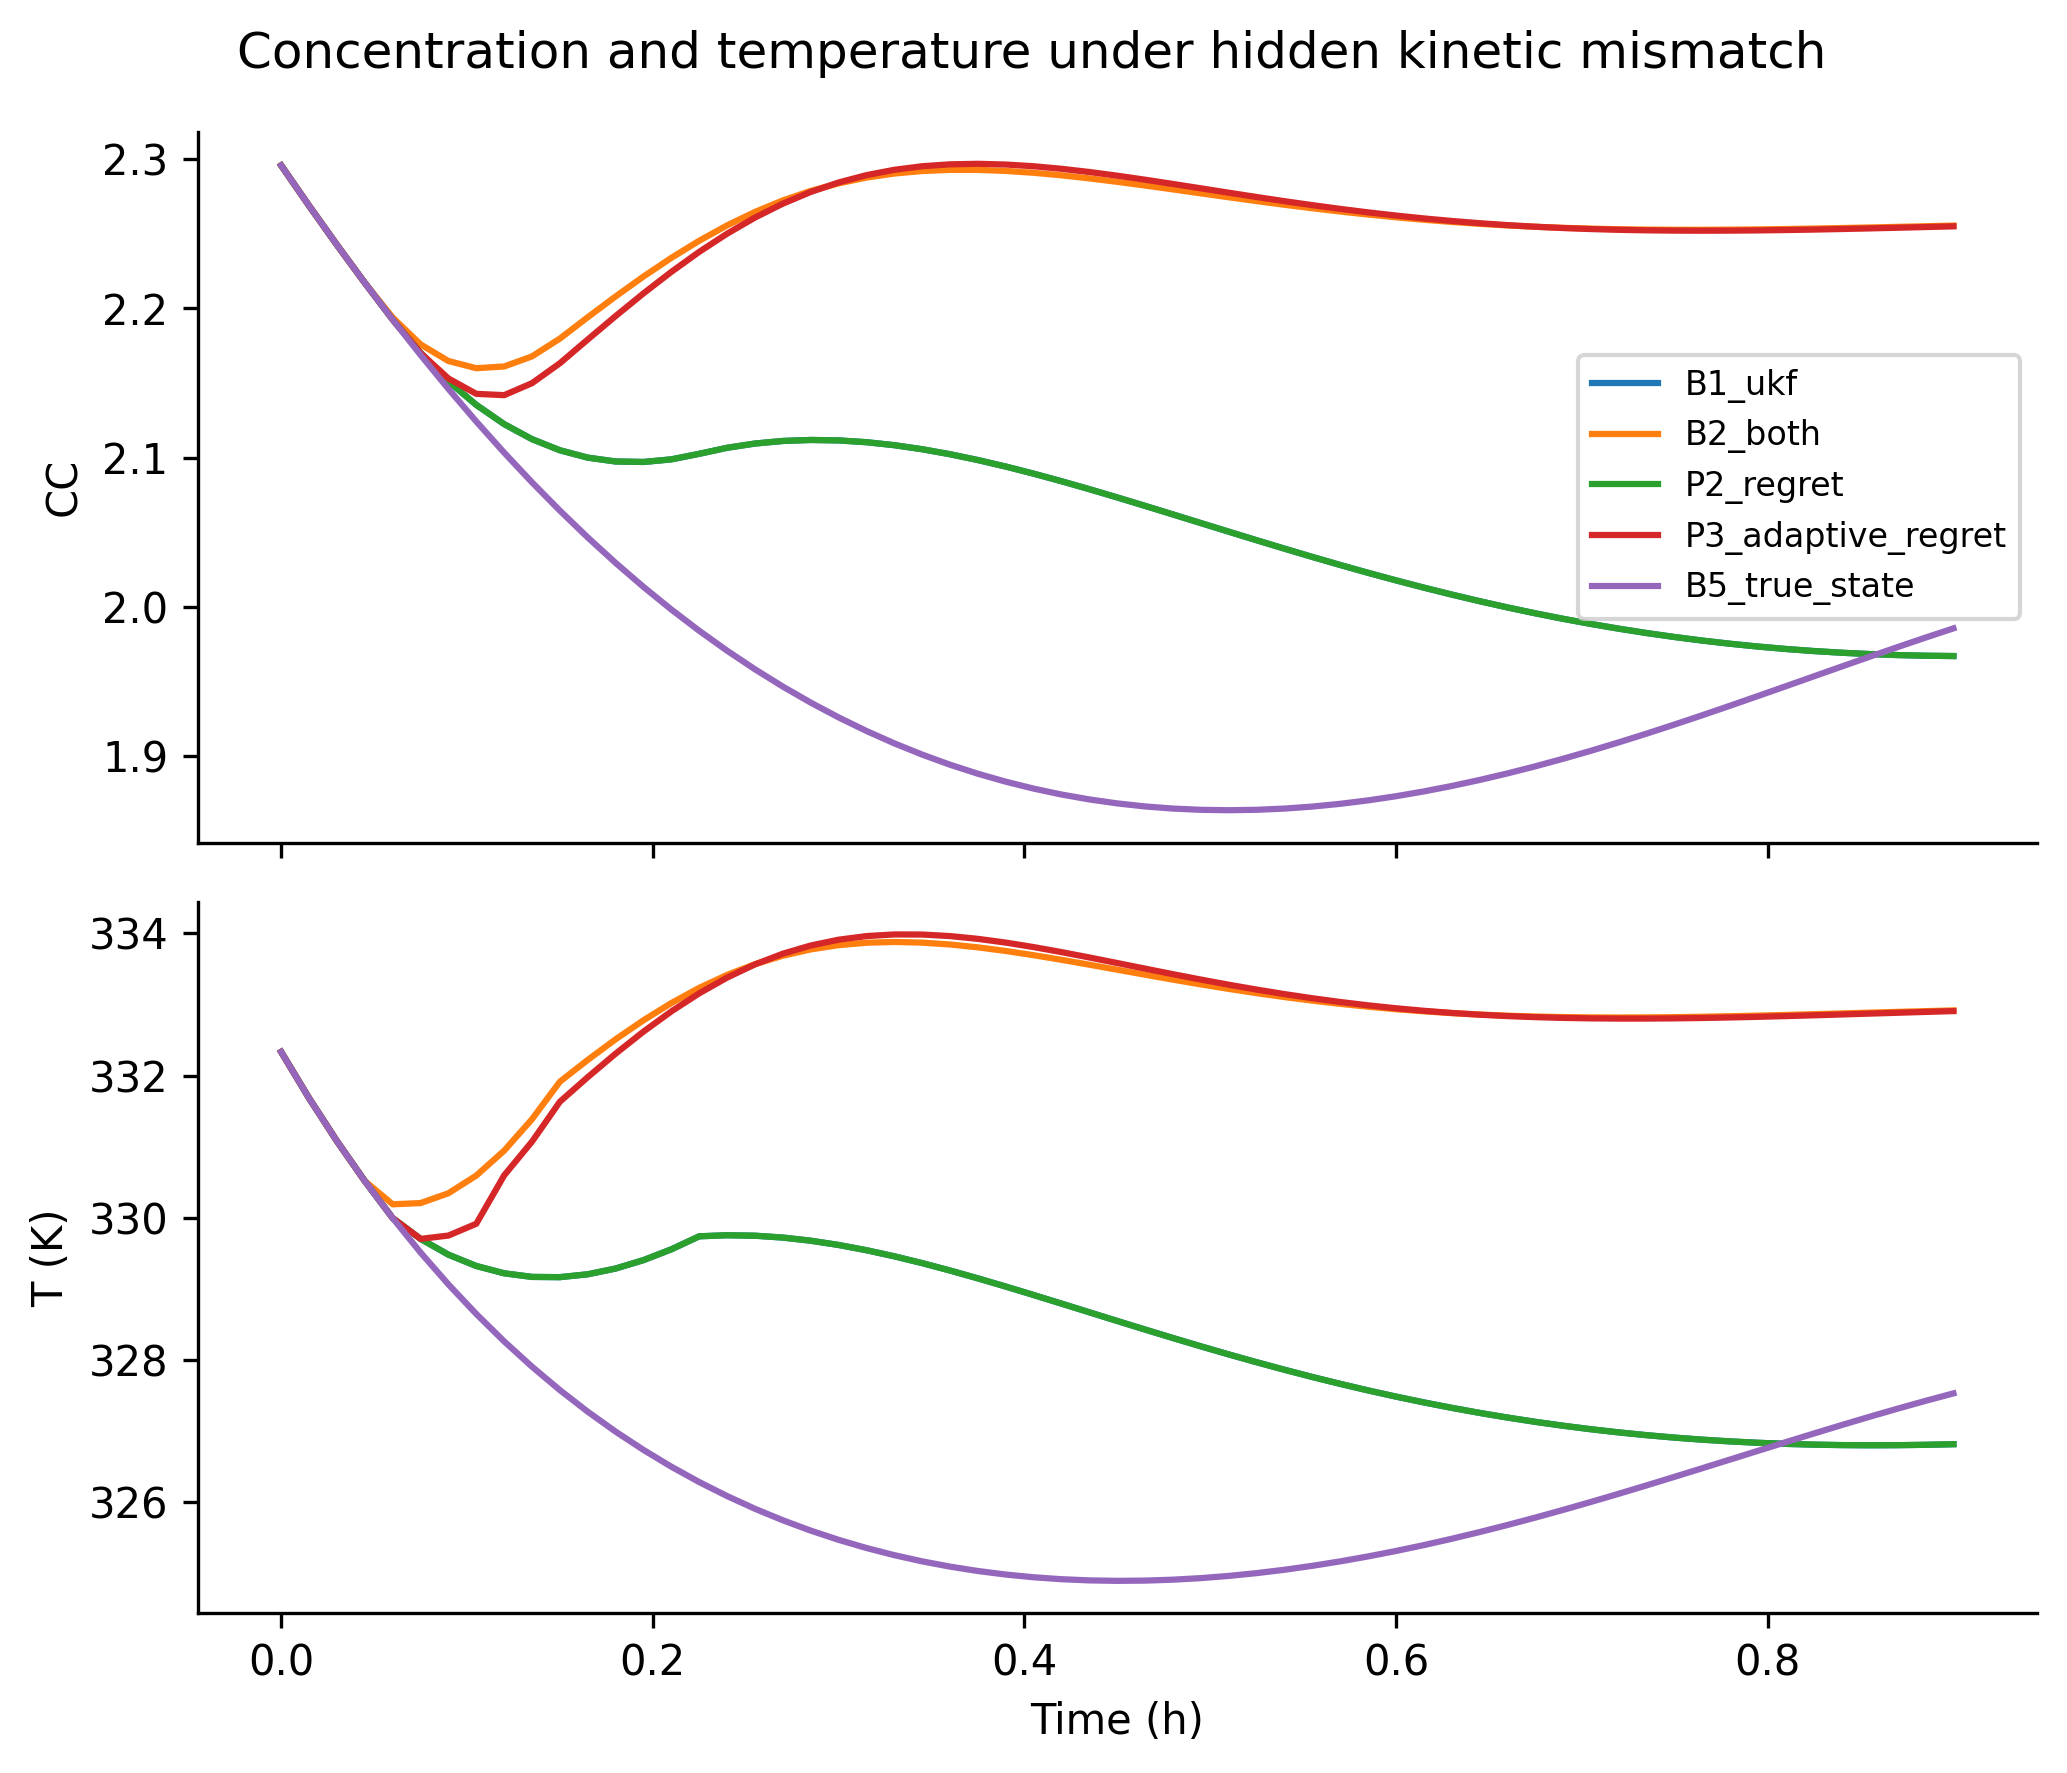
\includegraphics{figures/Figure_11.png}
\caption{Figure 11. Concentration and temperature under hidden kinetic
mismatch}
\end{figure}

\begin{figure}
\centering
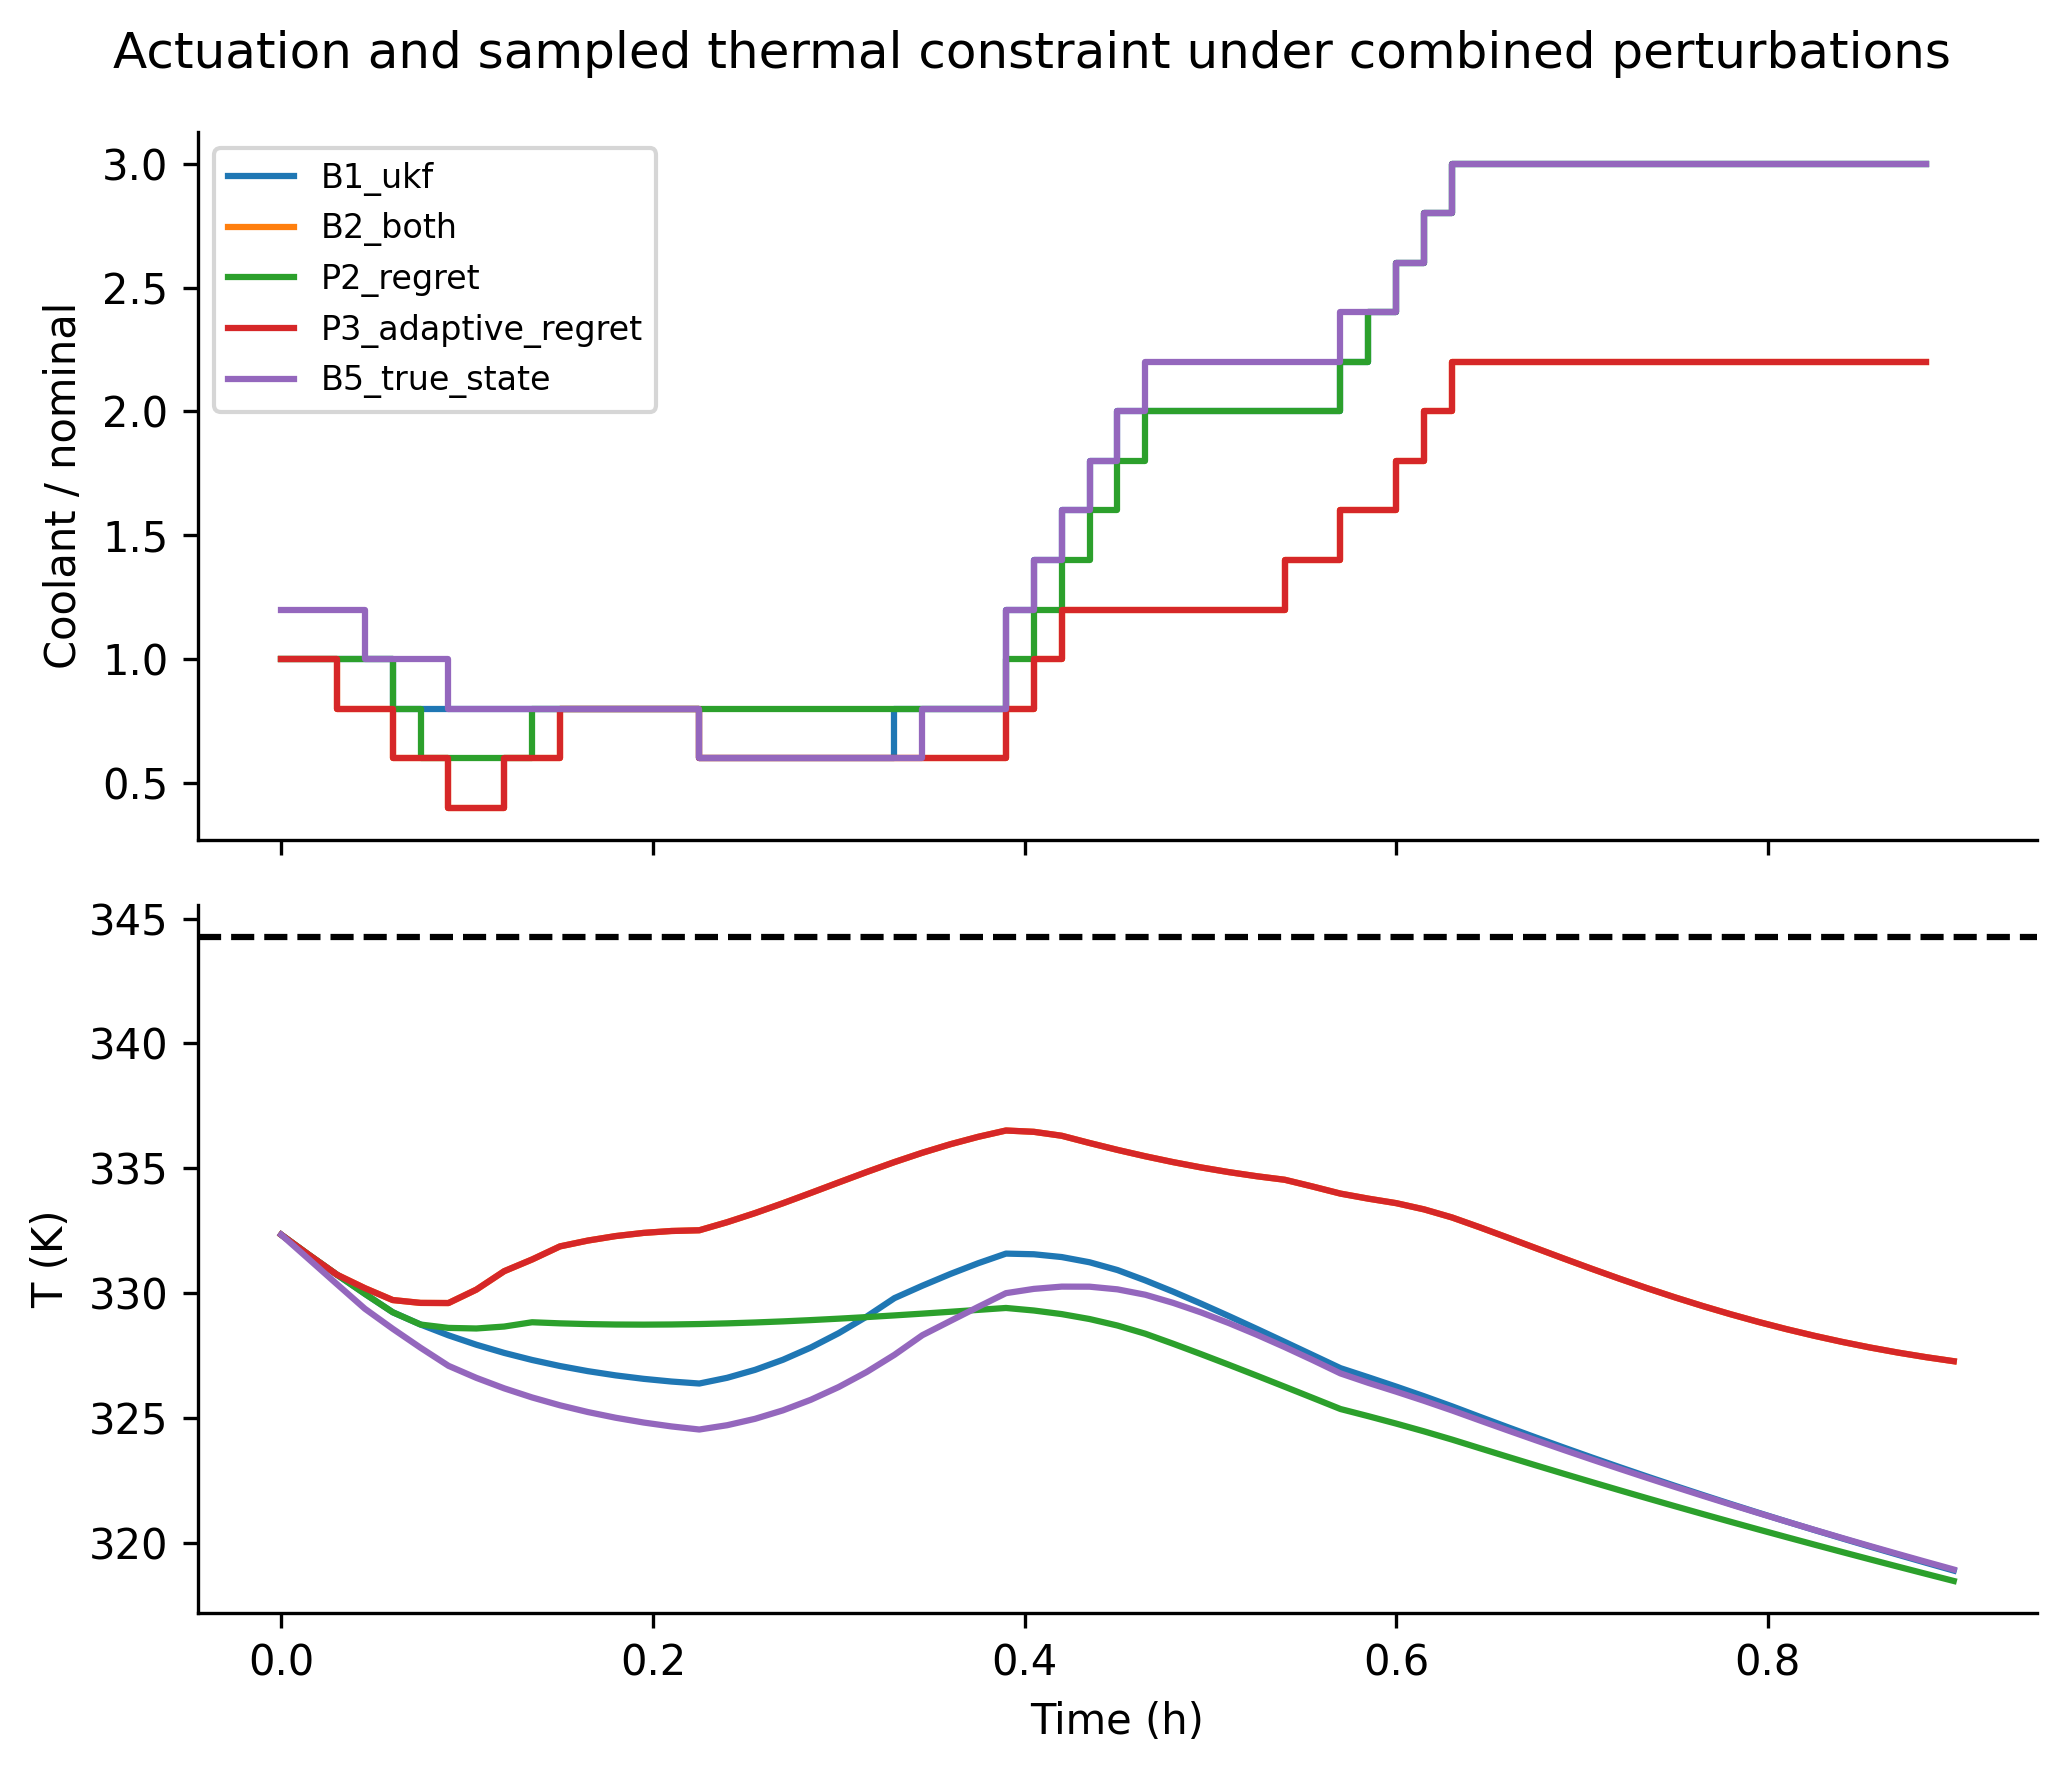
\includegraphics{figures/Figure_12.png}
\caption{Figure 12. Actuation and sampled thermal constraint under
combined perturbations}
\end{figure}

\begin{figure}
\centering
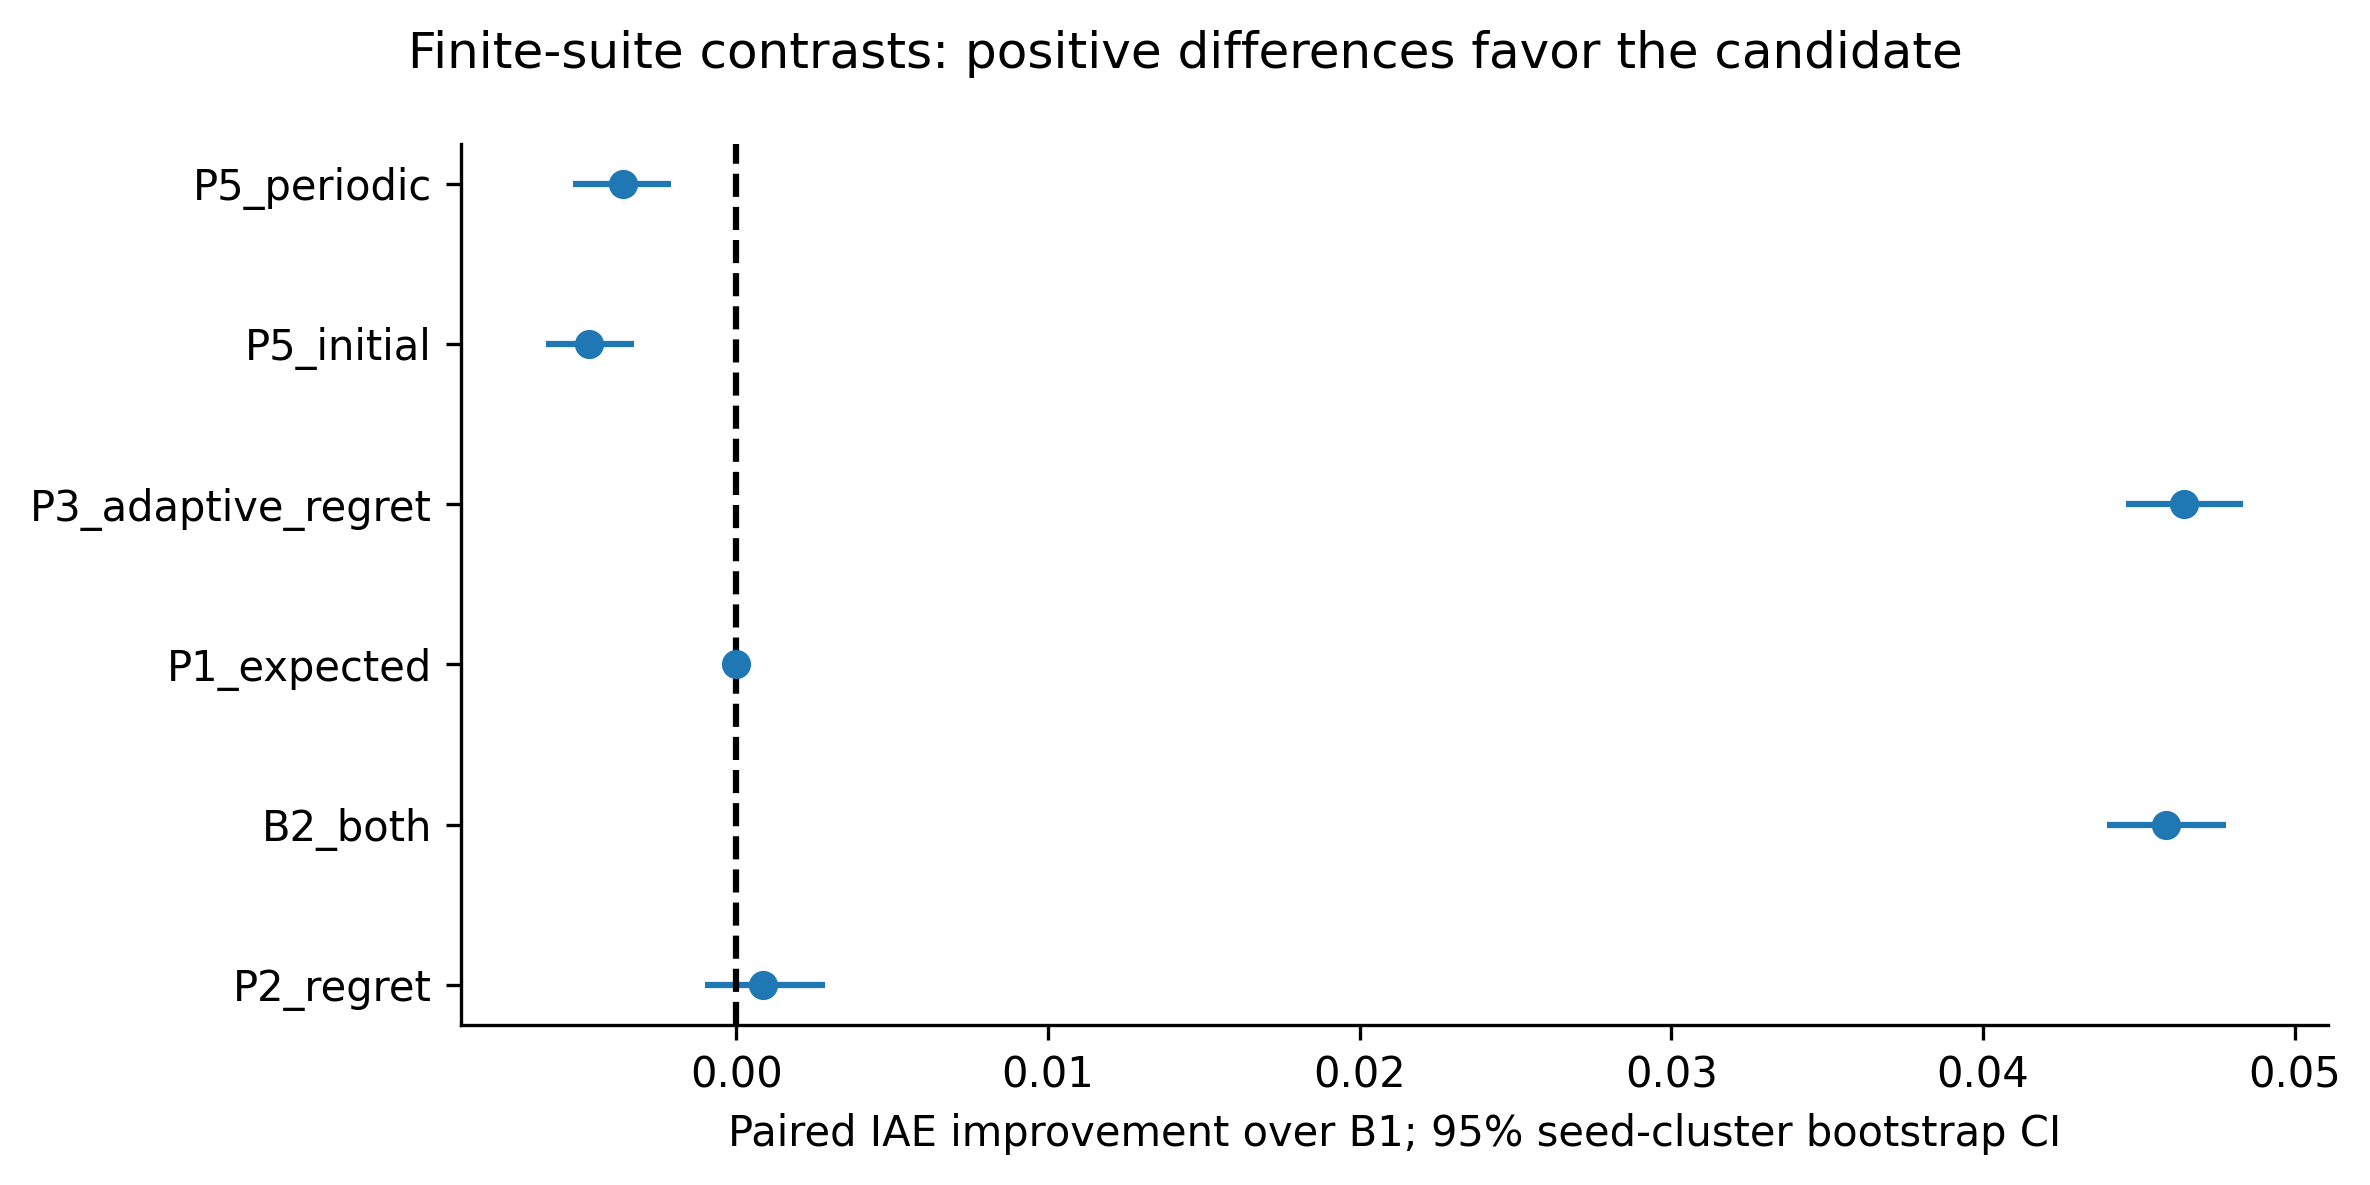
\includegraphics{figures/Figure_13.png}
\caption{Figure 13. Finite-suite contrasts: positive differences favor
the candidate}
\end{figure}

\begin{figure}
\centering
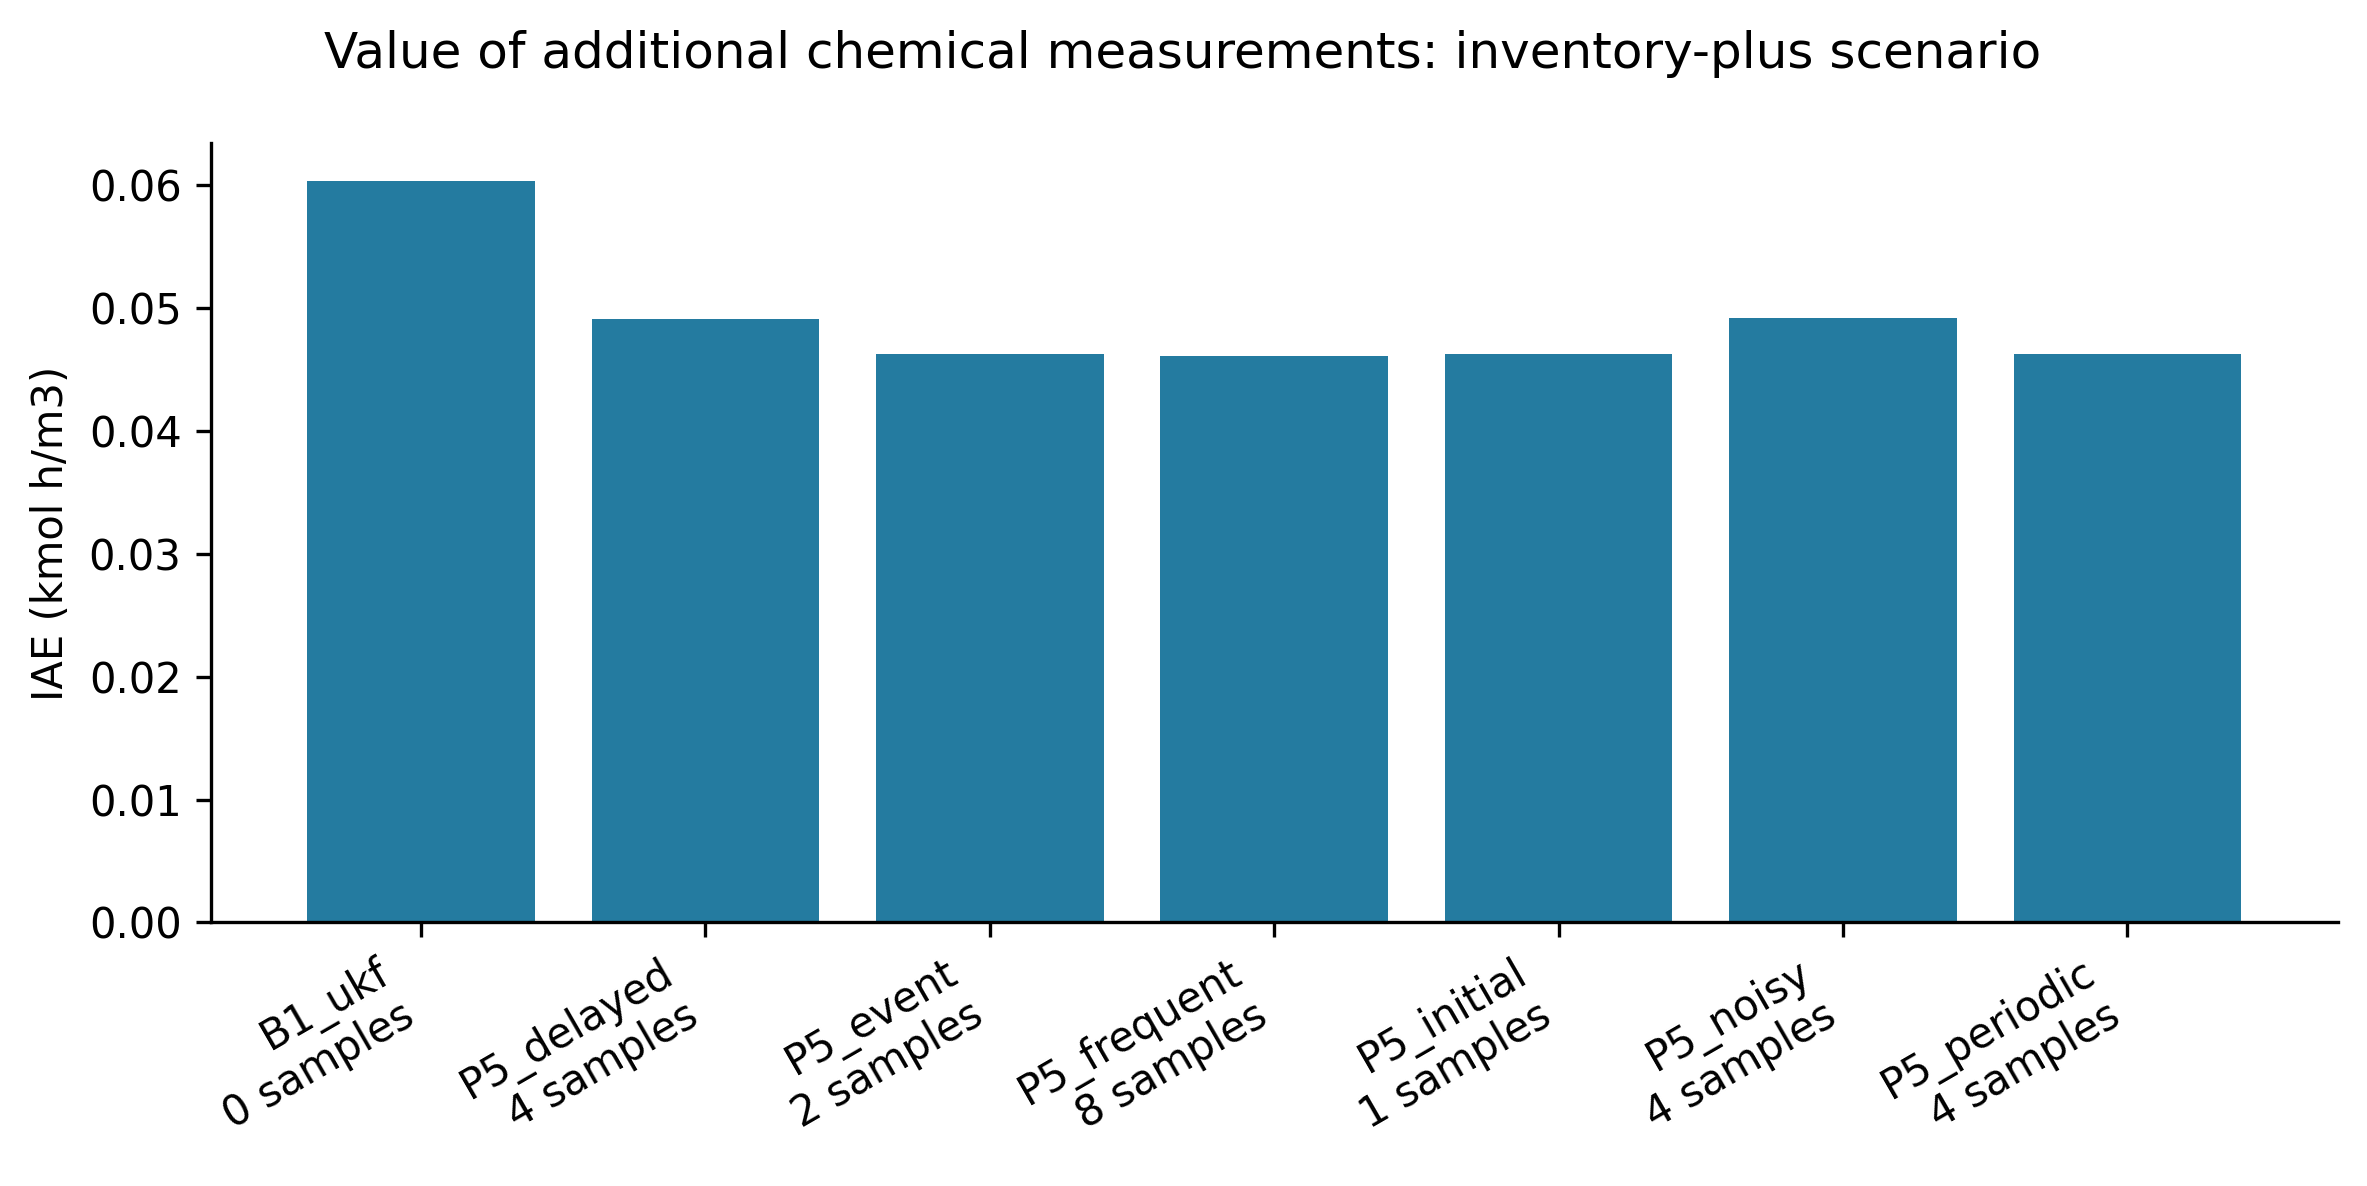
\includegraphics{figures/Figure_14.png}
\caption{Figure 14. Value of additional chemical measurements:
inventory-plus scenario}
\end{figure}

\begin{figure}
\centering
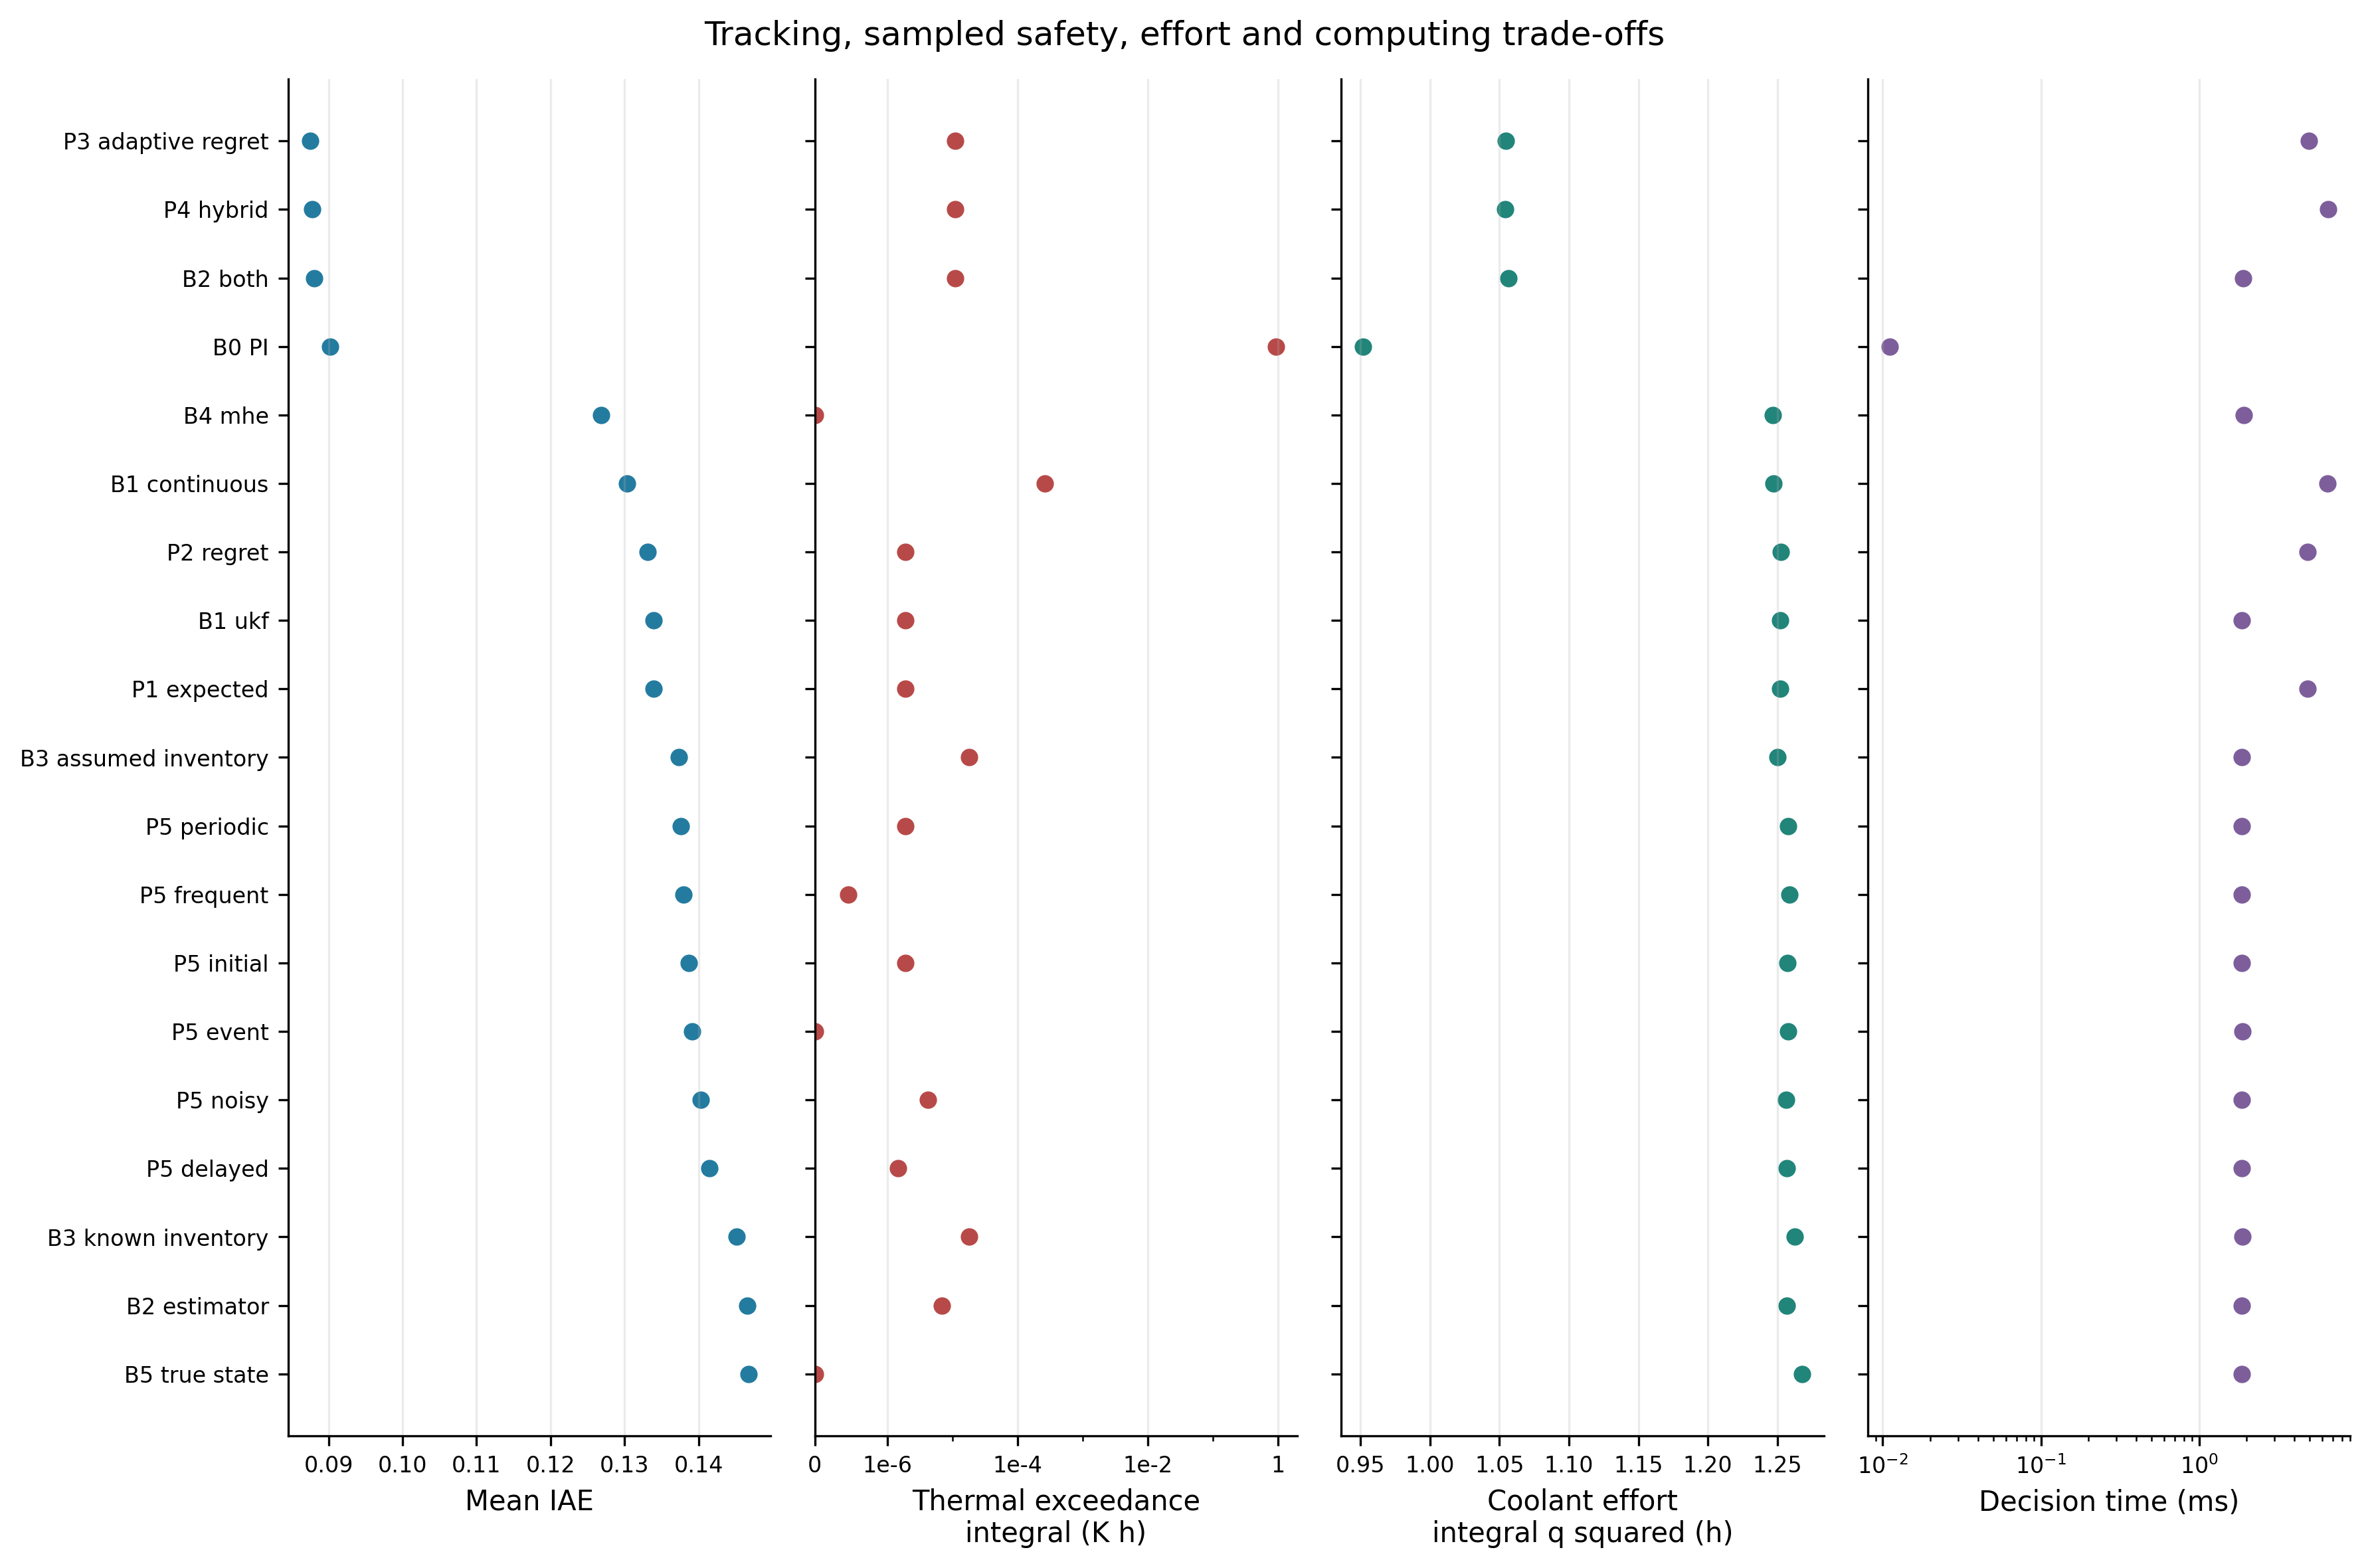
\includegraphics{figures/Figure_15.png}
\caption{Figure 15. Tracking, sampled safety, effort and computing
trade-offs}
\end{figure}

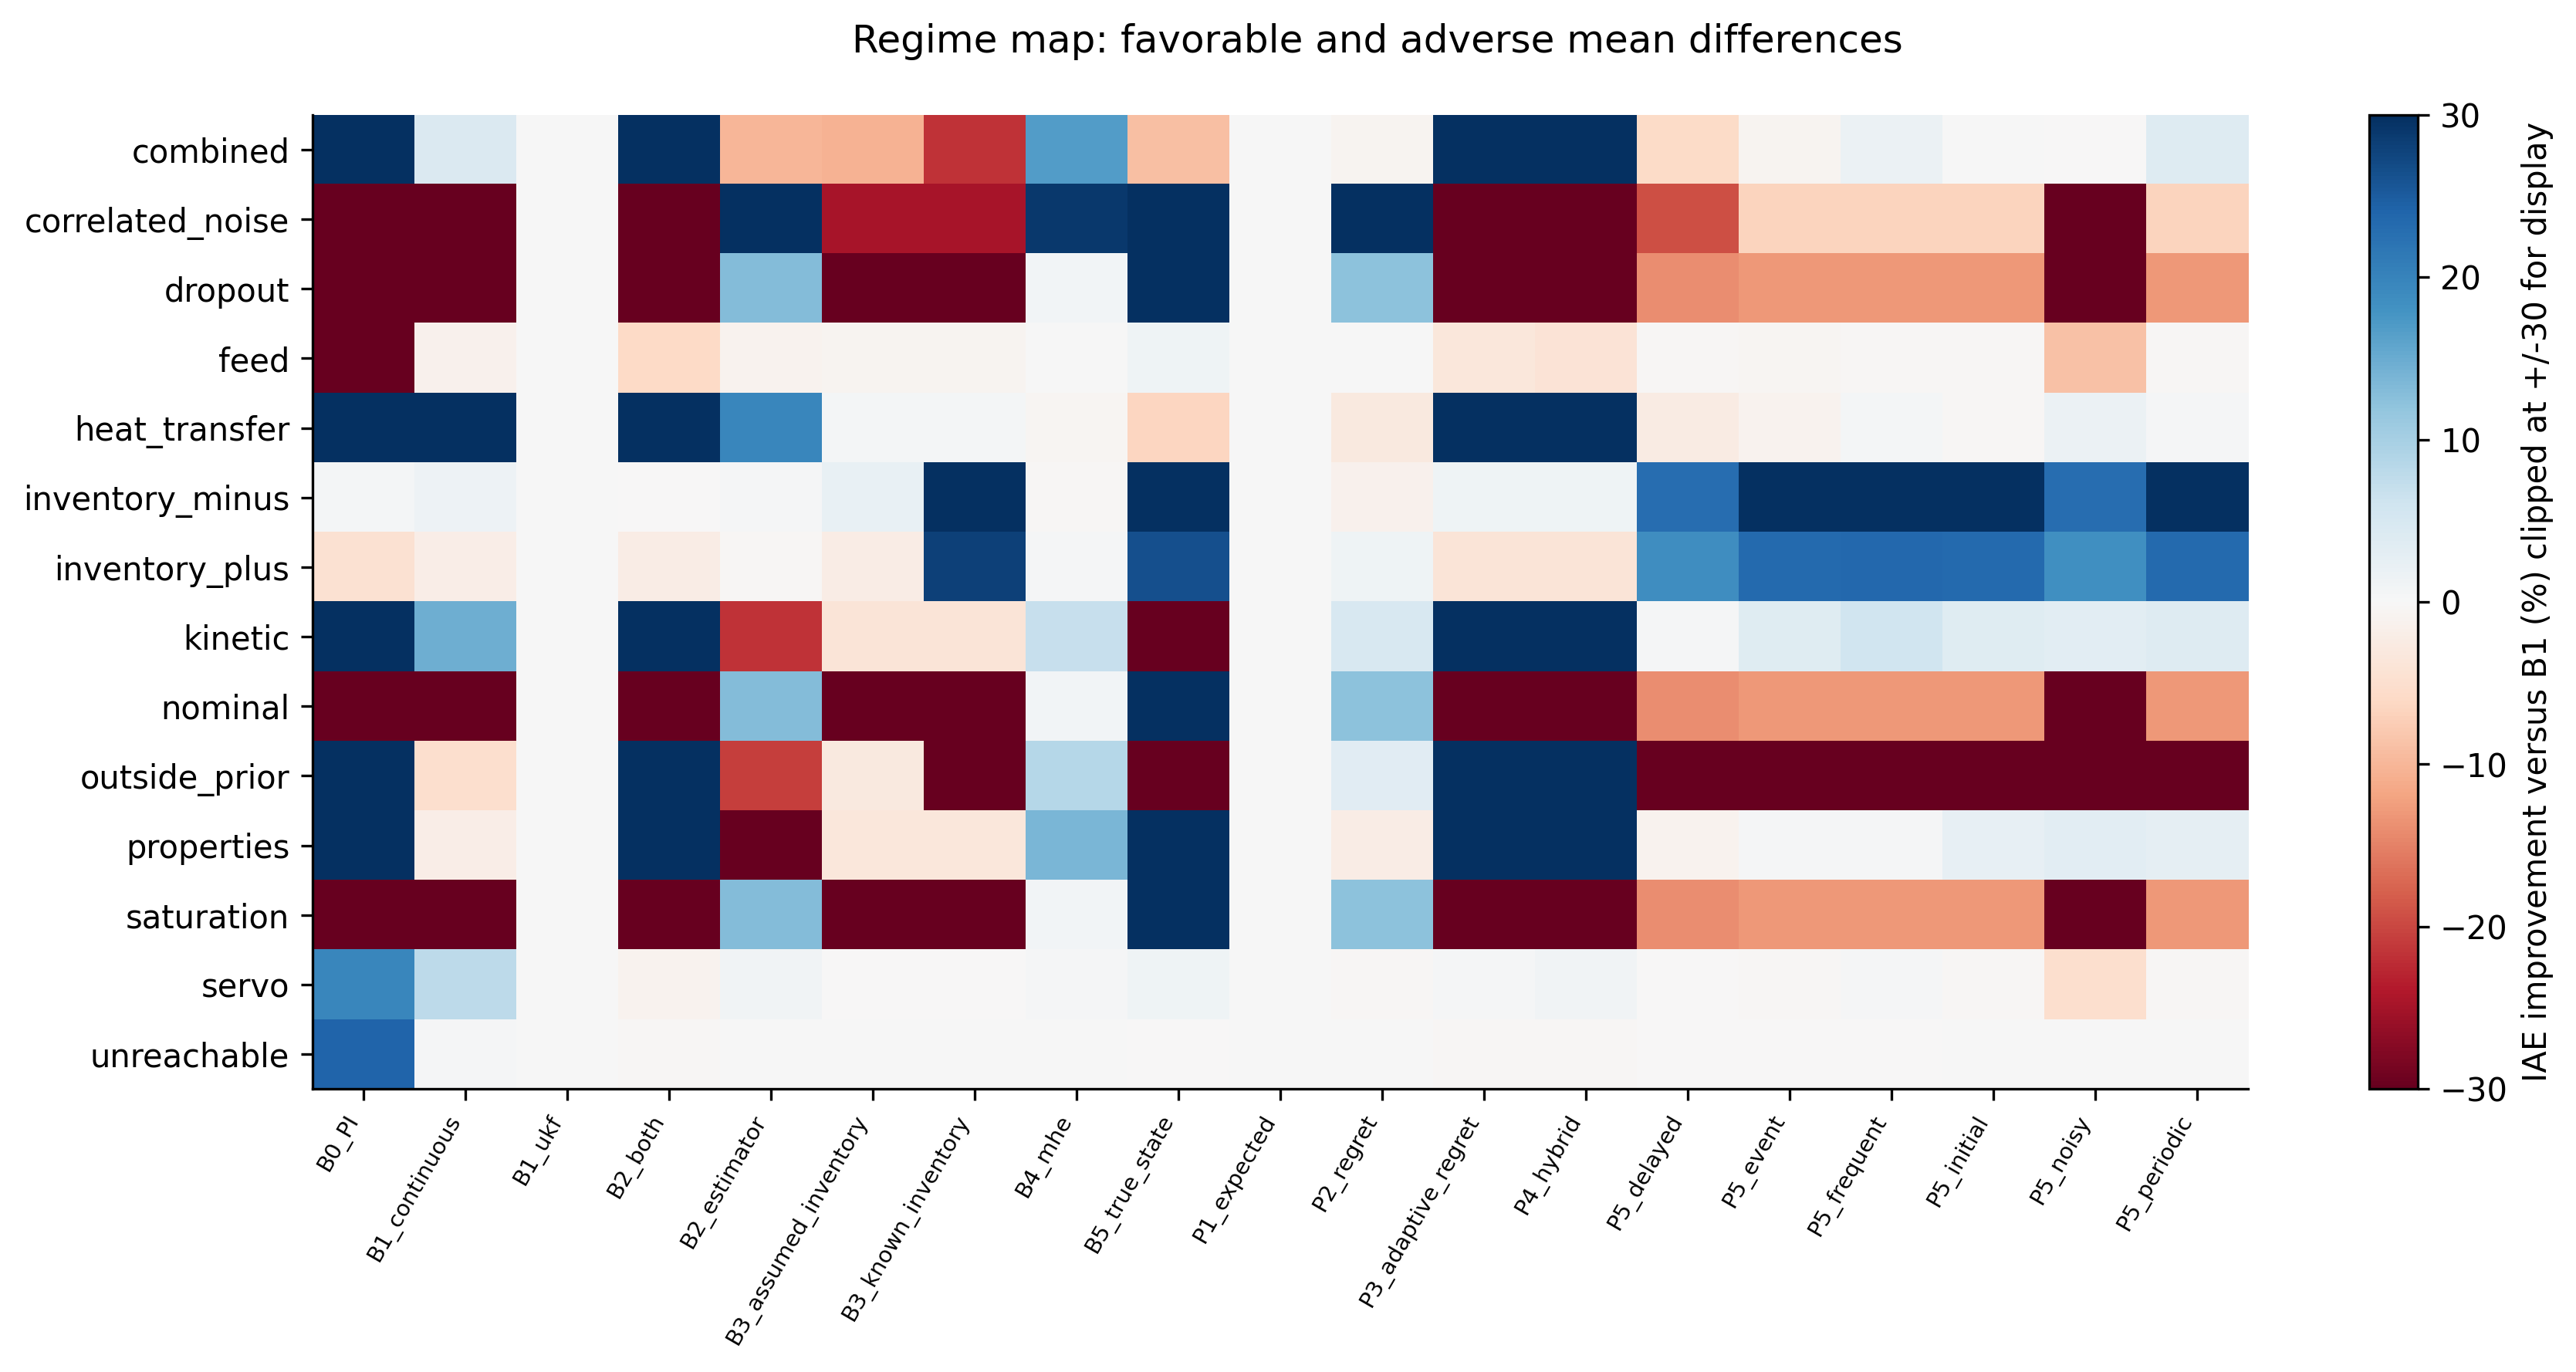
\includegraphics{figures/Figure_16.png} \# Referências

\hypertarget{auditoria-da-recuperauxe7uxe3o}{%
\section{Auditoria da
recuperação}\label{auditoria-da-recuperauxe7uxe3o}}

\hypertarget{recovery-audit-and-historical-status}{%
\section{Recovery audit and historical
status}\label{recovery-audit-and-historical-status}}

Reference date: 20 October 2026. Repository default main was
f4444d4c238291b8633743930249ee387ad94541. New campaign starts from
d2610a0723cbbaf00d3f4559242ba0efafb67771, which preserves the
Darwin/thesis sources.

\begin{longtable}[]{@{}
  >{\raggedright\arraybackslash}p{(\columnwidth - 4\tabcolsep) * \real{0.3333}}
  >{\raggedright\arraybackslash}p{(\columnwidth - 4\tabcolsep) * \real{0.3333}}
  >{\raggedright\arraybackslash}p{(\columnwidth - 4\tabcolsep) * \real{0.3333}}@{}}
\toprule\noalign{}
\begin{minipage}[b]{\linewidth}\raggedright
Material
\end{minipage} & \begin{minipage}[b]{\linewidth}\raggedright
Recovery
\end{minipage} & \begin{minipage}[b]{\linewidth}\raggedright
Scope
\end{minipage} \\
\midrule\noalign{}
\endhead
\bottomrule\noalign{}
\endlastfoot
Dissertation, Dissertacao\_WalterYanko.pdf & Text read, pp.38--42 &
Original balances, sensors, heat exchange and parameter table. 92-page
PDF; not all pages reread. \\
modeloCT.m & Full original source recovered & Literal six-state
historical dynamics \\
modeloFun\_KF.m, NMPC\_Fmincon.m, model/observer archive & Present in
traced Git tree & Some prior audit content and NMPC reconstruction read;
original MATLAB runtime not executed \\
Simulink package & Filename located, bytes unavailable locally & No
Simulink execution \\
Relatorio\_CSTR\_Propilenoglicol.pdf & Relevant physical and attribution
pages read & Historical values, units, seeds and caveats established \\
ICAC\_Manuscrito\_PT.pdf & Full five-page manuscript read & Historical
twin and decision claims \\
research/icac-information-decision & Absent from live branch listing;
commit search found no ICAC match & Code and full raw reproduction
unavailable \\
PG C01--C14 & Timeline in Relatorio\_Campanhas\_PG\_EB\_Arioston.pdf
read & Some C02/C03/C04/C12 code survives on beyond branch; no full
14-campaign replay \\
Darwin complete/thesis & Code and source manifest recovered from Git &
Existing outputs are inherited evidence, not new execution \\
Darwin reduced branch & Audit-only checkpoint recovered & It explicitly
reports zero new trajectories; not a completed reduced-model campaign \\
PG\_Darwin\_Reduced\_Pilot\_v0.1 & Report read; package identified &
Independent PI/EKF pilot, tabulated variant; not equivalent to
historical NMPC \\
PG Model Fidelity v0.8 & Current RESULTADOS.md v8 read & 1792 reported
episodes, oracle parameter interpolation; not causal online
identification \\
New frontier & Independent implementation with parity test & Its numbers
are not substitutions for the historical protocols \\
\end{longtable}

\begin{longtable}[]{@{}
  >{\raggedright\arraybackslash}p{(\columnwidth - 6\tabcolsep) * \real{0.2500}}
  >{\raggedright\arraybackslash}p{(\columnwidth - 6\tabcolsep) * \real{0.2500}}
  >{\raggedright\arraybackslash}p{(\columnwidth - 6\tabcolsep) * \real{0.2500}}
  >{\raggedright\arraybackslash}p{(\columnwidth - 6\tabcolsep) * \real{0.2500}}@{}}
\toprule\noalign{}
\begin{minipage}[b]{\linewidth}\raggedright
Historical result
\end{minipage} & \begin{minipage}[b]{\linewidth}\raggedright
Reported value
\end{minipage} & \begin{minipage}[b]{\linewidth}\raggedright
New exact reproduction
\end{minipage} & \begin{minipage}[b]{\linewidth}\raggedright
Divergence / status
\end{minipage} \\
\midrule\noalign{}
\endhead
\bottomrule\noalign{}
\endlastfoot
ICAC twin product gap & 0.426449 kmol/m3 & Not reproduced at that
historical endpoint & Construction/protocol raw files inaccessible; new
.4/.8 twin experiments use declared different initial conditions \\
Instantaneous lower bound & 0.213225 kmol/m3 & Analytic half-gap rule
verified; rounded historical scalar inherited & 0.426449/2=0.2132245
before rounding \\
Nominal predictor hidden mismatch IAE & 0.951143 kmol h/m3 & Not rerun &
Original 6 h, 400-step protocol differs from new 0.9 h episodes \\
Estimator-only correction IAE & 0.850912 & Not rerun & Source: PG report
pp.55--57; 20 seeds 270201--270220 \\
Estimator+predictor correction IAE & 0.358768 & Not rerun & Same
historical mismatch contrast; no new historical validation claim \\
ICAC B1 relative IAE & -14.60\% & Not rerun & Manuscript reports six
holdout seeds, different horizon/objective; not pooled with new data \\
\end{longtable}

\hypertarget{physical-changes}{%
\subsection{Physical changes}\label{physical-changes}}

The table's reaction heat is -91556.90 kJ/kmol; the executable uses
-36000 Btu/lbmol, converted in the recovered archive to -83736 kJ/kmol.
M0 uses the latter. The historical Fahrenheit +460 Arrhenius convention
becomes Kelvin +0.183333333333. Replacing it silently by exact absolute
temperature would change the benchmark.

M1H adds a Kirchhoff correction with an ASSUMED reference enthalpy at
nominal T. This is thermodynamically consistent within the chosen
ideal-mixture model but is not a physically calibrated reconciliation.
M1J adds a reciprocal lumped jacket, with conductance selected to match
the original nominal stationary coil duty. M2L and M2Q use declared
synthetic slopes/curvatures of species Cp(T). They are
sensitivity/falsification families, not measured property correlations.

The initial test run had 17 passes and one failed effect-size
expectation. The full record and scientific interpretation are preserved
in initial\_test\_failure.md.

\hypertarget{unexecuted-central-requirements}{%
\subsection{Unexecuted central
requirements}\label{unexecuted-central-requirements}}

Exact historical C08/ICAC replay; all C01--C14 raw audits; validated
physical-property M1; full continuous 57-step/6-move strong baseline;
fully tuned MHE; CPU timing on the target Ryzen; prospective
Lie-derivative symbolic rank sweep; independent human theoretical
review. These gaps prohibit labeling the entire requested v1.0 FINAL
complete.

\hypertarget{mixture-admissibility-gap}{%
\subsection{Mixture admissibility gap}\label{mixture-admissibility-gap}}

The benchmark uses constant volume and feed-based volumetric outflow
without a separately validated mixture equation of state or
partial-molar-volume constraint. Positive concentrations are admissible
to M0 but do not alone certify real-liquid composition admissibility.
Nonideal mixture enthalpy, reaction volume change and exact
composition-volume constraints remain uncalibrated. Their influence must
be assessed before making a physical impossibility claim.

\hypertarget{revisuxe3o-bibliogruxe1fica-cruxedtica}{%
\section{Revisão bibliográfica
crítica}\label{revisuxe3o-bibliogruxe1fica-cruxedtica}}

\hypertarget{critical-literature-review-20-october-2026}{%
\section{Critical literature review --- 20 October
2026}\label{critical-literature-review-20-october-2026}}

This is a targeted, source-verified review, not an exhaustive systematic
review. No worldwide novelty claim is justified by this search.
Publisher metadata, author-hosted manuscripts and institutional records
were preferred. Paywalls and inaccessible pages were recorded.

\begin{longtable}[]{@{}
  >{\raggedright\arraybackslash}p{(\columnwidth - 4\tabcolsep) * \real{0.3333}}
  >{\raggedright\arraybackslash}p{(\columnwidth - 4\tabcolsep) * \real{0.3333}}
  >{\raggedright\arraybackslash}p{(\columnwidth - 4\tabcolsep) * \real{0.3333}}@{}}
\toprule\noalign{}
\begin{minipage}[b]{\linewidth}\raggedright
Topic
\end{minipage} & \begin{minipage}[b]{\linewidth}\raggedright
Verified antecedent
\end{minipage} & \begin{minipage}[b]{\linewidth}\raggedright
Relation and limit of the present contribution
\end{minipage} \\
\midrule\noalign{}
\endhead
\bottomrule\noalign{}
\endlastfoot
Nonlinear observability & Hermann and Krener (1977), DOI
10.1109/TAC.1977.1101601 & Local rank conditions are established. Here
exact PG symmetry is proved directly; finite numerical rank is not
called structural proof. IEEE page had a robot gate. \\
Reactor indistinguishability & Schaum, Moreno, Díaz-Salgado and Alvarez,
IFAC DYCOPS 2007 & Nonmonotone kinetics already produce concentration
ambiguity with thermal sensing. Our PG construction instead uses
calorimetric compensation and shared dilution. \\
Identifiability & Villaverde, Barreiro and Papachristodoulou (2016), DOI
10.1371/journal.pcbi.1005153 & State augmentation and Lie-derivative
identifiability are established; this campaign does not invent that
analysis. \\
Empirical reduction/information & Lall, Marsden and Glavaski (2002), DOI
10.1002/rnc.657 & Trajectory sensitivity and empirical reduction have
long precedents. Our finite-horizon singular spectra are diagnostic, not
an exact global Gramian theorem. \\
MHE & Rao, Rawlings and Mayne (2003), DOI 10.1109/TAC.2002.808470 &
Constrained deterministic estimation has stability conditions. The
six-step implementation here does not establish those conditions or
represent a fully tuned best-in-class MHE. \\
Output-feedback MPC & Rawlings, Mayne and Diehl, second-edition
textbook, author site & Standard foundations and implementation
reference. State error, model error and constraints interact; new
guarantees are not inferred from trajectory plots. \\
Regret under measurements & Goel and Hassibi, PMLR 144 (2021),
1270--1280 & Prior regret-optimal linear control compares to an offline
benchmark. Here the comparator knows the initial chemical world but uses
the same finite action class; these regret definitions are different. \\
Decision-focused prediction & Elmachtoub and Grigas (2022), DOI
10.1287/mnsc.2020.3922 & Prediction error and decision loss need not
align. No novelty is claimed for that principle. Our setting is dynamic
inferential control. \\
Dual control & Klenske and Hennig, JMLR 17(127), 2016 & Actions may
change learning. The present scenario controller does not optimize
future observation distributions, so it is not a full dual
controller. \\
Belief MPC, recent & Cao et al., arXiv:2604.24663 (2026), preprint &
Linear dynamics, bilinear sensing and input-dependent Kalman covariance.
Its favorable synthetic results do not establish gains for this
nonlinear reactor. \\
Latent-risk planning, recent & Enwerem, Baras and Belta,
arXiv:2604.03868 v2 (2026), preprint & Measured state with latent
parameters, CVaR and MPPI. Our ambiguity is chemical state with thermal
observations; no CVaR guarantee is imported. \\
Reactor physics & Brandão dissertation (2019), pp.~30--32; recovered
modeloCT.m & Original six-state equations and sensors. Table/coded
enthalpies differ; M0 follows code and preserves its Arrhenius
offset. \\
Reaction enthalpy correction & Fogler, UMich living example 12-4 & The
public code contains a temperature correction from reaction Cp
difference. It supports checking Kirchhoff consistency, not importing
its different operating point or enthalpy as a calibrated
replacement. \\
\end{longtable}

Searches also covered set-membership nonlinear MPC (Canale, DOI
10.1002/rnc.2878; publisher full text was inaccessible), inferential
control, information-constrained control, value of chemical sampling and
chemical-reactor observability. Coverage of the entire 2025--2026
literature and full-text comparisons remains incomplete.

\hypertarget{claim-by-claim-originality-assessment}{%
\subsection{Claim-by-claim originality
assessment}\label{claim-by-claim-originality-assessment}}

\begin{enumerate}
\def\labelenumi{\arabic{enumi}.}
\tightlist
\item
  Two invisible chemical modes in the constant-Cp PG model:
  case-specific construction, already present in recovered internal ICAC
  material; not a new discovery of this campaign.
\item
  Persistence under a reciprocal jacket and consistent
  temperature-dependent reaction enthalpy: explicit extension of that
  construction; potentially useful audit result.
\item
  Dimension controlled by the span of species heat-capacity functions:
  candidate compact structural characterization. Priority not
  established; compare against general quotient systems, reaction
  invariants and structural-identifiability literature before claiming
  novelty.
\item
  Half-separation estimation bound and convex regret bound: elementary
  consequences of known inequalities, not independent major theoretical
  novelty.
\item
  Controller superiority: must be determined by paired test and
  confirmation data, including adverse regimes, stronger continuous
  baselines, safety and computation.
\item
  Publication: a reproducible negative or mixed result may be valuable.
  Submission readiness still requires recovered historical replay,
  better physical properties, stronger baselines and independent expert
  review.
\end{enumerate}

All bibliography entries are in manuscripts/references.bib. Preprints
are explicitly labeled.

\hypertarget{additional-physical-source-check}{%
\subsection{Additional physical source
check}\label{additional-physical-source-check}}

Chan and Seider (University of Pennsylvania, July 2004) use excess-water
first-order kinetics and nonideal-liquid thermodynamics in a related
batch teaching case. These assumptions differ from a calibrated CSTR
model. A 2026 microchannel-kinetics paper at
https://www.mdpi.com/2227-9717/14/9/1491 was located, but the publisher
returned HTTP 429; its parameters were not imported. This is an access
limitation, not evidence against alternative kinetics.

\hypertarget{configurauxe7uxe3o-congelada}{%
\section{Configuração congelada}\label{configurauxe7uxe3o-congelada}}

\begin{Shaded}
\begin{Highlighting}[]
\FunctionTok{\{}
  \DataTypeTok{"version"}\FunctionTok{:} \StringTok{"1.0{-}computational{-}core"}\FunctionTok{,}
  \DataTypeTok{"date"}\FunctionTok{:} \StringTok{"2026{-}10{-}20"}\FunctionTok{,}
  \DataTypeTok{"status"}\FunctionTok{:} \StringTok{"frozen before new simulations"}\FunctionTok{,}
  \DataTypeTok{"scope"}\FunctionTok{:} \StringTok{"Historical M0 benchmark and explicitly hypothetical reconciliations; no industrial validation"}\FunctionTok{,}
  \DataTypeTok{"development\_seeds"}\FunctionTok{:} \OtherTok{[}
    \DecValTok{11}\OtherTok{,}
    \DecValTok{12}
  \OtherTok{]}\FunctionTok{,}
  \DataTypeTok{"validation\_seeds"}\FunctionTok{:} \OtherTok{[}
    \DecValTok{101}\OtherTok{,}
    \DecValTok{102}\OtherTok{,}
    \DecValTok{103}
  \OtherTok{]}\FunctionTok{,}
  \DataTypeTok{"test\_seeds"}\FunctionTok{:} \OtherTok{[}
    \DecValTok{4100}\OtherTok{,}
    \DecValTok{4101}\OtherTok{,}
    \DecValTok{4102}\OtherTok{,}
    \DecValTok{4103}\OtherTok{,}
    \DecValTok{4104}\OtherTok{,}
    \DecValTok{4105}\OtherTok{,}
    \DecValTok{4106}\OtherTok{,}
    \DecValTok{4107}\OtherTok{,}
    \DecValTok{4108}\OtherTok{,}
    \DecValTok{4109}\OtherTok{,}
    \DecValTok{4110}\OtherTok{,}
    \DecValTok{4111}\OtherTok{,}
    \DecValTok{4112}\OtherTok{,}
    \DecValTok{4113}\OtherTok{,}
    \DecValTok{4114}\OtherTok{,}
    \DecValTok{4115}\OtherTok{,}
    \DecValTok{4116}\OtherTok{,}
    \DecValTok{4117}\OtherTok{,}
    \DecValTok{4118}\OtherTok{,}
    \DecValTok{4119}
  \OtherTok{]}\FunctionTok{,}
  \DataTypeTok{"confirmation\_seeds"}\FunctionTok{:} \OtherTok{[}
    \DecValTok{8100}\OtherTok{,}
    \DecValTok{8101}\OtherTok{,}
    \DecValTok{8102}\OtherTok{,}
    \DecValTok{8103}\OtherTok{,}
    \DecValTok{8104}\OtherTok{,}
    \DecValTok{8105}\OtherTok{,}
    \DecValTok{8106}\OtherTok{,}
    \DecValTok{8107}\OtherTok{,}
    \DecValTok{8108}\OtherTok{,}
    \DecValTok{8109}\OtherTok{,}
    \DecValTok{8110}\OtherTok{,}
    \DecValTok{8111}\OtherTok{,}
    \DecValTok{8112}\OtherTok{,}
    \DecValTok{8113}\OtherTok{,}
    \DecValTok{8114}\OtherTok{,}
    \DecValTok{8115}\OtherTok{,}
    \DecValTok{8116}\OtherTok{,}
    \DecValTok{8117}\OtherTok{,}
    \DecValTok{8118}\OtherTok{,}
    \DecValTok{8119}
  \OtherTok{]}\FunctionTok{,}
  \DataTypeTok{"dt\_h"}\FunctionTok{:} \FloatTok{0.015}\FunctionTok{,}
  \DataTypeTok{"steps"}\FunctionTok{:} \DecValTok{60}\FunctionTok{,}
  \DataTypeTok{"horizon"}\FunctionTok{:} \DecValTok{14}\FunctionTok{,}
  \DataTypeTok{"grid\_points\_per\_move"}\FunctionTok{:} \DecValTok{5}\FunctionTok{,}
  \DataTypeTok{"move\_blocks"}\FunctionTok{:} \OtherTok{[}
    \DecValTok{3}\OtherTok{,}
    \DecValTok{11}
  \OtherTok{]}\FunctionTok{,}
  \DataTypeTok{"qmin"}\FunctionTok{:} \FloatTok{0.05}\FunctionTok{,}
  \DataTypeTok{"qmax"}\FunctionTok{:} \DecValTok{3}\FunctionTok{,}
  \DataTypeTok{"slew"}\FunctionTok{:} \FloatTok{0.4}\FunctionTok{,}
  \DataTypeTok{"study\_T\_limit"}\FunctionTok{:} \FloatTok{344.2611111111}\FunctionTok{,}
  \DataTypeTok{"primary\_contrasts"}\FunctionTok{:} \OtherTok{[}
    \OtherTok{[}
      \StringTok{"P2\_regret"}\OtherTok{,}
      \StringTok{"B1\_ukf"}
    \OtherTok{],}
    \OtherTok{[}
      \StringTok{"P3\_adaptive\_regret"}\OtherTok{,}
      \StringTok{"B2\_both"}
    \OtherTok{],}
    \OtherTok{[}
      \StringTok{"B2\_both"}\OtherTok{,}
      \StringTok{"B2\_estimator"}
    \OtherTok{]}
  \OtherTok{]}\FunctionTok{,}
  \DataTypeTok{"primary\_metric"}\FunctionTok{:} \StringTok{"paired trajectory IAE"}\FunctionTok{,}
  \DataTypeTok{"uncertainty"}\FunctionTok{:} \StringTok{"20 independent paired noise seeds within each fixed scenario; seed{-}cluster bootstrap across finite scenario suite"}\FunctionTok{,}
  \DataTypeTok{"success\_rule"}\FunctionTok{:} \StringTok{"exploratory target \textgreater{}=10\% IAE improvement with 95\% paired CI above zero, no material increase in thermal severity, confirmation; multiplicity Holm for three primary contrasts"}\FunctionTok{,}
  \DataTypeTok{"information"}\FunctionTok{:} \StringTok{"Only current T,Tt, past actions and measured current feeds. No future disturbances. Exact{-}inventory and chemical variants separately labeled."}\FunctionTok{,}
  \DataTypeTok{"runtime\_budget"}\FunctionTok{:} \StringTok{"one CPU worker; 60 min job ceiling; pilot predicts cost; do not silently trim seeds"}\FunctionTok{,}
  \DataTypeTok{"model\_variants"}\FunctionTok{:} \StringTok{"M0 historical. M1H Kirchhoff with assumed reaction{-}enthalpy reference at nominal T; M1J adds nominally matched lumped jacket; M2L/Q synthetic cp(T) slopes/curvatures, not measured properties."}\FunctionTok{,}
  \DataTypeTok{"gaps"}\FunctionTok{:} \StringTok{"ICAC branch absent at recovery; C01{-}C14 raw code not retrieved; historical scalar values not automatically reproduced."}
\FunctionTok{\}}
\end{Highlighting}
\end{Shaded}

\hypertarget{registro-de-testes}{%
\section{Registro de testes}\label{registro-de-testes}}

\begin{verbatim}
test_01_historical_rhs_parity (test_science.ScientificTests.test_01_historical_rhs_parity) ... ok
test_02_conserved_reaction_inventories (test_science.ScientificTests.test_02_conserved_reaction_inventories) ... ok
test_03_energy_accounting (test_science.ScientificTests.test_03_energy_accounting) ... ok
test_04_equilibrium (test_science.ScientificTests.test_04_equilibrium) ... ok
test_05_positivity (test_science.ScientificTests.test_05_positivity) ... ok
test_06_independent_integration (test_science.ScientificTests.test_06_independent_integration) ... ok
test_07_jacobian_step_consistency (test_science.ScientificTests.test_07_jacobian_step_consistency) ... ok
test_08_twins_constant_cp_and_jacket (test_science.ScientificTests.test_08_twins_constant_cp_and_jacket) ... ok
test_09_variable_cp_falsifies_specific_twin (test_science.ScientificTests.test_09_variable_cp_falsifies_specific_twin) ... ok
test_10_rank_has_two_exact_null_directions (test_science.ScientificTests.test_10_rank_has_two_exact_null_directions) ... ok
test_11_causal_prefix (test_science.ScientificTests.test_11_causal_prefix) ... ok
test_12_inventory_reconstruction (test_science.ScientificTests.test_12_inventory_reconstruction) ... ok
test_13_constraints (test_science.ScientificTests.test_13_constraints) ... ok
test_14_failed_optimization_fallback (test_science.ScientificTests.test_14_failed_optimization_fallback) ... ok
test_15_regret_exact (test_science.ScientificTests.test_15_regret_exact) ... ok
test_16_zero_conflict_not_impossible_state_error (test_science.ScientificTests.test_16_zero_conflict_not_impossible_state_error) ... ok
test_17_seed_separation (test_science.ScientificTests.test_17_seed_separation) ... ok
test_18_reproducible_and_metric_independent (test_science.ScientificTests.test_18_reproducible_and_metric_independent) ... ok

----------------------------------------------------------------------
Ran 18 tests in 11.990s

OK
\end{verbatim}

\hypertarget{verificauxe7uxe3o-independente-de-muxe9tricas}{%
\section{Verificação independente de
métricas}\label{verificauxe7uxe3o-independente-de-muxe9tricas}}

\begin{Shaded}
\begin{Highlighting}[]
\FunctionTok{\{}
  \DataTypeTok{"trajectories\_checked"}\FunctionTok{:} \DecValTok{5720}\FunctionTok{,}
  \DataTypeTok{"trajectories\_expected"}\FunctionTok{:} \DecValTok{5720}\FunctionTok{,}
  \DataTypeTok{"max\_iae\_error"}\FunctionTok{:} \FloatTok{9.8879238130678e{-}17}\FunctionTok{,}
  \DataTypeTok{"max\_rmse\_error"}\FunctionTok{:} \FloatTok{9.8879238130678e{-}17}\FunctionTok{,}
  \DataTypeTok{"pass\_all"}\FunctionTok{:} \KeywordTok{true}
\FunctionTok{\}}
\end{Highlighting}
\end{Shaded}

\hypertarget{todos-os-cenuxe1rios-muxe9dias-por-muxe9todo}{%
\section{Todos os cenários: médias por
método}\label{todos-os-cenuxe1rios-muxe9dias-por-muxe9todo}}

\begin{longtable}[]{@{}
  >{\raggedright\arraybackslash}p{(\columnwidth - 16\tabcolsep) * \real{0.1111}}
  >{\raggedright\arraybackslash}p{(\columnwidth - 16\tabcolsep) * \real{0.1111}}
  >{\raggedright\arraybackslash}p{(\columnwidth - 16\tabcolsep) * \real{0.1111}}
  >{\raggedright\arraybackslash}p{(\columnwidth - 16\tabcolsep) * \real{0.1111}}
  >{\raggedright\arraybackslash}p{(\columnwidth - 16\tabcolsep) * \real{0.1111}}
  >{\raggedright\arraybackslash}p{(\columnwidth - 16\tabcolsep) * \real{0.1111}}
  >{\raggedright\arraybackslash}p{(\columnwidth - 16\tabcolsep) * \real{0.1111}}
  >{\raggedright\arraybackslash}p{(\columnwidth - 16\tabcolsep) * \real{0.1111}}
  >{\raggedright\arraybackslash}p{(\columnwidth - 16\tabcolsep) * \real{0.1111}}@{}}
\toprule\noalign{}
\begin{minipage}[b]{\linewidth}\raggedright
scenario
\end{minipage} & \begin{minipage}[b]{\linewidth}\raggedright
method
\end{minipage} & \begin{minipage}[b]{\linewidth}\raggedright
IAE
\end{minipage} & \begin{minipage}[b]{\linewidth}\raggedright
RMSE\_CC
\end{minipage} & \begin{minipage}[b]{\linewidth}\raggedright
Tmax
\end{minipage} & \begin{minipage}[b]{\linewidth}\raggedright
thermal\_severity
\end{minipage} & \begin{minipage}[b]{\linewidth}\raggedright
fallback
\end{minipage} & \begin{minipage}[b]{\linewidth}\raggedright
decision\_ms
\end{minipage} & \begin{minipage}[b]{\linewidth}\raggedright
samples
\end{minipage} \\
\midrule\noalign{}
\endhead
\bottomrule\noalign{}
\endlastfoot
combined & B0\_PI & 0.0934287 & 0.121056 & 335.189 & 0 & 0 & 0.0110679 &
0 \\
combined & B1\_continuous & 0.220454 & 0.130548 & 332.334 & 0 & 0 &
4.96751 & 0 \\
combined & B1\_ukf & 0.230553 & 0.130567 & 332.353 & 0 & 0 & 1.66006 &
0 \\
combined & B2\_both & 0.0797465 & 0.0764126 & 337.065 & 0 & 0 & 1.90273
& 0 \\
combined & B2\_estimator & 0.253608 & 0.077038 & 332.334 & 0 & 0 &
1.67091 & 0 \\
combined & B3\_assumed\_inventory & 0.254337 & 0.120627 & 332.334 & 0 &
0 & 1.68198 & 0 \\
combined & B3\_known\_inventory & 0.280497 & 0.131838 & 332.334 & 0 & 0
& 1.67366 & 0 \\
combined & B4\_mhe & 0.191722 & 0.118114 & 332.58 & 0 & 0 & 1.71293 &
0 \\
combined & B5\_true\_state & 0.251169 & 0 & 332.334 & 0 & 0 & 1.66569 &
0 \\
combined & P1\_expected & 0.230553 & 0.130567 & 332.353 & 0 & 0 & 4.3434
& 0 \\
combined & P2\_regret & 0.232497 & 0.130859 & 332.334 & 0 & 0 & 4.27689
& 0 \\
combined & P3\_adaptive\_regret & 0.078689 & 0.0763533 & 337.167 & 0 & 0
& 4.95168 & 0 \\
combined & P4\_hybrid & 0.0809885 & 0.0764077 & 337.047 & 0 & 0 &
6.53605 & 0 \\
combined & P5\_delayed & 0.243523 & 0.124689 & 332.334 & 0 & 0 & 1.66562
& 4 \\
combined & P5\_event & 0.23268 & 0.110226 & 332.34 & 0 & 0 & 1.66652 &
3.2 \\
combined & P5\_frequent & 0.226337 & 0.101357 & 332.34 & 0 & 0 & 1.66237
& 8 \\
combined & P5\_initial & 0.230523 & 0.111119 & 332.342 & 0 & 0 & 1.66955
& 1 \\
combined & P5\_noisy & 0.230777 & 0.119001 & 332.37 & 0 & 0 & 1.66112 &
4 \\
combined & P5\_periodic & 0.221859 & 0.105677 & 332.334 & 0 & 0 &
1.65882 & 4 \\
correlated\_noise & B0\_PI & 0.0123505 & 0.0189866 & 333.33 & 0 & 0 &
0.0108627 & 0 \\
correlated\_noise & B1\_continuous & 0.00562245 & 0.0191299 & 332.768 &
0 & 0 & 5.0819 & 0 \\
correlated\_noise & B1\_ukf & 0.00178324 & 0.0193683 & 332.458 & 0 & 0 &
1.94382 & 0 \\
correlated\_noise & B2\_both & 0.00889772 & 0.0255135 & 333.221 & 0 & 0
& 1.95377 & 0 \\
correlated\_noise & B2\_estimator & 0.00106716 & 0.0253827 & 332.406 & 0
& 0 & 1.92291 & 0 \\
correlated\_noise & B3\_assumed\_inventory & 0.00222358 & 0.0180951 &
332.599 & 0 & 0 & 1.9298 & 0 \\
correlated\_noise & B3\_known\_inventory & 0.00222358 & 0.0180951 &
332.599 & 0 & 0 & 1.93739 & 0 \\
correlated\_noise & B4\_mhe & 0.00126539 & 0.0201908 & 332.396 & 0 & 0 &
1.97049 & 0 \\
correlated\_noise & B5\_true\_state & 0 & 0 & 332.334 & 0 & 0 & 1.91732
& 0 \\
correlated\_noise & P1\_expected & 0.00178324 & 0.0193683 & 332.458 & 0
& 0 & 5.00956 & 0 \\
correlated\_noise & P2\_regret & 0.00118565 & 0.0192305 & 332.42 & 0 & 0
& 5.008 & 0 \\
correlated\_noise & P3\_adaptive\_regret & 0.00775816 & 0.0253758 &
333.203 & 0 & 0 & 5.08538 & 0 \\
correlated\_noise & P4\_hybrid & 0.00821111 & 0.0254199 & 333.268 & 0 &
0 & 6.74898 & 0 \\
correlated\_noise & P5\_delayed & 0.0021283 & 0.019508 & 332.477 & 0 & 0
& 1.92068 & 4 \\
correlated\_noise & P5\_event & 0.00190228 & 0.0213424 & 332.473 & 0 & 0
& 1.9474 & 2 \\
correlated\_noise & P5\_frequent & 0.00190228 & 0.0199258 & 332.473 & 0
& 0 & 1.91933 & 8 \\
correlated\_noise & P5\_initial & 0.00190228 & 0.0219477 & 332.473 & 0 &
0 & 1.92563 & 1 \\
correlated\_noise & P5\_noisy & 0.00621623 & 0.0464674 & 332.833 & 0 & 0
& 1.91554 & 4 \\
correlated\_noise & P5\_periodic & 0.00190228 & 0.0213421 & 332.473 & 0
& 0 & 1.92537 & 4 \\
dropout & B0\_PI & 0.00668463 & 0.0113724 & 332.932 & 0 & 0 & 0.0109944
& 0 \\
dropout & B1\_continuous & 0.00324538 & 0.0113149 & 332.612 & 0 & 0 &
5.00651 & 0 \\
dropout & B1\_ukf & 0.00164715 & 0.0113113 & 332.442 & 0 & 0 & 1.95127 &
0 \\
dropout & B2\_both & 0.00699446 & 0.0158507 & 332.895 & 0 & 0 & 1.96138
& 0 \\
dropout & B2\_estimator & 0.00143415 & 0.0158424 & 332.439 & 0 & 0 &
1.93105 & 0 \\
dropout & B3\_assumed\_inventory & 0.00233413 & 0.0114881 & 332.575 & 0
& 0 & 1.93689 & 0 \\
dropout & B3\_known\_inventory & 0.00233413 & 0.0114881 & 332.575 & 0 &
0 & 1.93007 & 0 \\
dropout & B4\_mhe & 0.00163409 & 0.0121761 & 332.429 & 0 & 0 & 1.97396 &
0 \\
dropout & B5\_true\_state & 0 & 0 & 332.334 & 0 & 0 & 1.91165 & 0 \\
dropout & P1\_expected & 0.00164715 & 0.0113113 & 332.442 & 0 & 0 &
5.00011 & 0 \\
dropout & P2\_regret & 0.00144464 & 0.0113217 & 332.372 & 0 & 0 &
4.97137 & 0 \\
dropout & P3\_adaptive\_regret & 0.00606505 & 0.0158336 & 332.894 & 0 &
0 & 5.11531 & 0 \\
dropout & P4\_hybrid & 0.00643227 & 0.0158296 & 332.909 & 0 & 0 & 6.7783
& 0 \\
dropout & P5\_delayed & 0.00187537 & 0.0126409 & 332.459 & 0 & 0 &
1.91053 & 4 \\
dropout & P5\_event & 0.00186214 & 0.0149296 & 332.446 & 0 & 0 & 1.94742
& 2 \\
dropout & P5\_frequent & 0.00186214 & 0.014337 & 332.446 & 0 & 0 &
1.92503 & 8 \\
dropout & P5\_initial & 0.00186214 & 0.0152763 & 332.446 & 0 & 0 &
1.91341 & 1 \\
dropout & P5\_noisy & 0.00792647 & 0.0429567 & 332.984 & 0 & 0 & 1.91463
& 4 \\
dropout & P5\_periodic & 0.00186214 & 0.0150989 & 332.446 & 0 & 0 &
1.92709 & 4 \\
feed & B0\_PI & 0.116105 & 0.0112358 & 336.78 & 0 & 0 & 0.011034 & 0 \\
feed & B1\_continuous & 0.0601001 & 0.0118731 & 332.604 & 0 & 0 &
4.44668 & 0 \\
feed & B1\_ukf & 0.0593563 & 0.0118769 & 332.437 & 0 & 0 & 1.62817 &
0 \\
feed & B2\_both & 0.0629218 & 0.0158988 & 332.925 & 0 & 0 & 1.63324 &
0 \\
feed & B2\_estimator & 0.0599657 & 0.015842 & 332.434 & 0 & 0 & 1.62384
& 0 \\
feed & B3\_assumed\_inventory & 0.0597743 & 0.0120298 & 332.574 & 0 & 0
& 1.61753 & 0 \\
feed & B3\_known\_inventory & 0.0597743 & 0.0120298 & 332.574 & 0 & 0 &
1.6278 & 0 \\
feed & B4\_mhe & 0.0593365 & 0.0128832 & 332.422 & 0 & 0 & 1.666 & 0 \\
feed & B5\_true\_state & 0.058536 & 0 & 332.334 & 0 & 0 & 1.61899 & 0 \\
feed & P1\_expected & 0.0593563 & 0.0118769 & 332.437 & 0 & 0 & 4.09111
& 0 \\
feed & P2\_regret & 0.059297 & 0.0118861 & 332.357 & 0 & 0 & 4.07328 &
0 \\
feed & P3\_adaptive\_regret & 0.0614349 & 0.015872 & 332.894 & 0 & 0 &
4.11717 & 0 \\
feed & P4\_hybrid & 0.0617339 & 0.0158851 & 332.909 & 0 & 0 & 5.47818 &
0 \\
feed & P5\_delayed & 0.059577 & 0.013194 & 332.452 & 0 & 0 & 1.62629 &
4 \\
feed & P5\_event & 0.0596464 & 0.0154435 & 332.439 & 0 & 0 & 1.62821 &
2.95 \\
feed & P5\_frequent & 0.0596269 & 0.0147917 & 332.439 & 0 & 0 & 1.61566
& 8 \\
feed & P5\_initial & 0.0595382 & 0.0157482 & 332.439 & 0 & 0 & 1.61276 &
1 \\
feed & P5\_noisy & 0.0645499 & 0.0431702 & 332.945 & 0 & 0 & 1.62767 &
4 \\
feed & P5\_periodic & 0.0595258 & 0.0155513 & 332.439 & 0 & 0 & 1.60685
& 4 \\
heat\_transfer & B0\_PI & 0.0314431 & 0.0229198 & 332.518 & 0 & 0 &
0.010955 & 0 \\
heat\_transfer & B1\_continuous & 0.0667541 & 0.0238628 & 332.334 & 0 &
0 & 5.60661 & 0 \\
heat\_transfer & B1\_ukf & 0.0997877 & 0.0245583 & 332.36 & 0 & 0 &
1.93389 & 0 \\
heat\_transfer & B2\_both & 0.0280007 & 0.0146261 & 333.88 & 0 & 0 &
1.96848 & 0 \\
heat\_transfer & B2\_estimator & 0.0802266 & 0.0157829 & 332.384 & 0 & 0
& 1.93719 & 0 \\
heat\_transfer & B3\_assumed\_inventory & 0.0992348 & 0.0271709 &
332.361 & 0 & 0 & 1.94852 & 0 \\
heat\_transfer & B3\_known\_inventory & 0.0992348 & 0.0271709 & 332.361
& 0 & 0 & 1.94609 & 0 \\
heat\_transfer & B4\_mhe & 0.100362 & 0.0198224 & 332.36 & 0 & 0 &
1.98089 & 0 \\
heat\_transfer & B5\_true\_state & 0.106194 & 0 & 332.334 & 0 & 0 &
1.9214 & 0 \\
heat\_transfer & P1\_expected & 0.0997877 & 0.0245583 & 332.36 & 0 & 0 &
5.02487 & 0 \\
heat\_transfer & P2\_regret & 0.102638 & 0.0246025 & 332.422 & 0 & 0 &
5.00644 & 0 \\
heat\_transfer & P3\_adaptive\_regret & 0.0304075 & 0.014657 & 333.893 &
0 & 0 & 5.12647 & 0 \\
heat\_transfer & P4\_hybrid & 0.0281281 & 0.0146108 & 333.872 & 0 & 0 &
6.92229 & 0 \\
heat\_transfer & P5\_delayed & 0.102189 & 0.0249363 & 332.366 & 0 & 0 &
1.9242 & 4 \\
heat\_transfer & P5\_event & 0.10081 & 0.0261589 & 332.373 & 0 & 0 &
1.94134 & 2 \\
heat\_transfer & P5\_frequent & 0.0990872 & 0.0245488 & 332.38 & 0 & 0 &
1.94438 & 8 \\
heat\_transfer & P5\_initial & 0.100252 & 0.0262812 & 332.38 & 0 & 0 &
1.92069 & 1 \\
heat\_transfer & P5\_noisy & 0.0979392 & 0.0483927 & 332.604 & 0 & 0 &
1.92941 & 4 \\
heat\_transfer & P5\_periodic & 0.0995364 & 0.0255886 & 332.38 & 0 & 0 &
1.91986 & 4 \\
inventory\_minus & B0\_PI & 0.0601428 & 0.120026 & 332.927 & 0 & 0 &
0.0110904 & 0 \\
inventory\_minus & B1\_continuous & 0.0595766 & 0.120164 & 332.612 & 0 &
0 & 4.96987 & 0 \\
inventory\_minus & B1\_ukf & 0.0604643 & 0.120222 & 332.442 & 0 & 0 &
1.92646 & 0 \\
inventory\_minus & B2\_both & 0.0605474 & 0.121061 & 332.925 & 0 & 0 &
1.9689 & 0 \\
inventory\_minus & B2\_estimator & 0.0603069 & 0.121246 & 332.439 & 0 &
0 & 1.93127 & 0 \\
inventory\_minus & B3\_assumed\_inventory & 0.0591603 & 0.123619 &
332.575 & 0 & 0 & 1.93347 & 0 \\
inventory\_minus & B3\_known\_inventory & 0.038648 & 0.0524107 & 336.442
& 0 & 0 & 1.92908 & 0 \\
inventory\_minus & B4\_mhe & 0.0606387 & 0.119864 & 332.429 & 0 & 0 &
1.96844 & 0 \\
inventory\_minus & B5\_true\_state & 0.0422572 & 0 & 335.358 & 0 & 0 &
1.92195 & 0 \\
inventory\_minus & P1\_expected & 0.0604643 & 0.120222 & 332.442 & 0 & 0
& 5.0301 & 0 \\
inventory\_minus & P2\_regret & 0.0612922 & 0.120322 & 332.372 & 0 & 0 &
5.03329 & 0 \\
inventory\_minus & P3\_adaptive\_regret & 0.0596605 & 0.121095 & 332.894
& 0 & 0 & 5.08718 & 0 \\
inventory\_minus & P4\_hybrid & 0.0596493 & 0.121085 & 332.909 & 0 & 0 &
6.77859 & 0 \\
inventory\_minus & P5\_delayed & 0.0466391 & 0.0824441 & 334.915 & 0 & 0
& 1.93842 & 4 \\
inventory\_minus & P5\_event & 0.0414219 & 0.0146262 & 335.822 & 0 & 0 &
1.93396 & 2 \\
inventory\_minus & P5\_frequent & 0.04162 & 0.014029 & 335.871 & 0 & 0 &
1.9336 & 8 \\
inventory\_minus & P5\_initial & 0.0417729 & 0.014942 & 335.857 & 0 & 0
& 1.91811 & 1 \\
inventory\_minus & P5\_noisy & 0.0465969 & 0.0441151 & 335.409 & 0 & 0 &
1.9186 & 4 \\
inventory\_minus & P5\_periodic & 0.0417729 & 0.0148061 & 335.857 & 0 &
0 & 1.92416 & 4 \\
inventory\_plus & B0\_PI & 0.063136 & 0.122461 & 332.927 & 0 & 0 &
0.0110245 & 0 \\
inventory\_plus & B1\_continuous & 0.0615694 & 0.122312 & 332.612 & 0 &
0 & 4.96386 & 0 \\
inventory\_plus & B1\_ukf & 0.0603865 & 0.122254 & 332.442 & 0 & 0 &
1.92123 & 0 \\
inventory\_plus & B2\_both & 0.0617974 & 0.122231 & 332.925 & 0 & 0 &
1.94594 & 0 \\
inventory\_plus & B2\_estimator & 0.060544 & 0.122043 & 332.439 & 0 & 0
& 1.91785 & 0 \\
inventory\_plus & B3\_assumed\_inventory & 0.0616905 & 0.11896 & 332.575
& 0 & 0 & 1.93792 & 0 \\
inventory\_plus & B3\_known\_inventory & 0.0435352 & 0.0522537 & 332.776
& 0 & 0 & 1.9344 & 0 \\
inventory\_plus & B4\_mhe & 0.0602121 & 0.122743 & 332.429 & 0 & 0 &
1.96823 & 0 \\
inventory\_plus & B5\_true\_state & 0.0444614 & 0 & 332.716 & 0 & 0 &
1.9173 & 0 \\
inventory\_plus & P1\_expected & 0.0603865 & 0.122254 & 332.442 & 0 & 0
& 5.01 & 0 \\
inventory\_plus & P2\_regret & 0.059559 & 0.122162 & 332.372 & 0 & 0 &
5.00578 & 0 \\
inventory\_plus & P3\_adaptive\_regret & 0.0626549 & 0.122186 & 332.894
& 0 & 0 & 5.08821 & 0 \\
inventory\_plus & P4\_hybrid & 0.0627469 & 0.122201 & 332.909 & 0 & 0 &
6.77881 & 0 \\
inventory\_plus & P5\_delayed & 0.0491223 & 0.0814387 & 332.675 & 0 & 0
& 1.93067 & 4 \\
inventory\_plus & P5\_event & 0.0462917 & 0.01508 & 332.697 & 0 & 0 &
1.93708 & 2 \\
inventory\_plus & P5\_frequent & 0.0461057 & 0.0144976 & 332.709 & 0 & 0
& 1.92228 & 8 \\
inventory\_plus & P5\_initial & 0.0462972 & 0.0154738 & 332.698 & 0 & 0
& 1.9196 & 1 \\
inventory\_plus & P5\_noisy & 0.0492122 & 0.0439567 & 332.647 & 0 & 0 &
1.92292 & 4 \\
inventory\_plus & P5\_periodic & 0.0462972 & 0.0153022 & 332.698 & 0 & 0
& 1.91706 & 4 \\
kinetic & B0\_PI & 0.0894276 & 0.0766046 & 333.276 & 0 & 0 & 0.0109034 &
0 \\
kinetic & B1\_continuous & 0.16428 & 0.081211 & 332.334 & 0 & 0 &
5.68928 & 0 \\
kinetic & B1\_ukf & 0.192631 & 0.0839044 & 332.334 & 0 & 0 & 1.93156 &
0 \\
kinetic & B2\_both & 0.0448606 & 0.0153278 & 333.993 & 0 & 0 & 1.98638 &
0 \\
kinetic & B2\_estimator & 0.234377 & 0.0168838 & 332.334 & 0 & 0 &
1.94017 & 0 \\
kinetic & B3\_assumed\_inventory & 0.199984 & 0.0940751 & 332.334 & 0 &
0 & 1.94387 & 0 \\
kinetic & B3\_known\_inventory & 0.199984 & 0.0940751 & 332.334 & 0 & 0
& 1.95366 & 0 \\
kinetic & B4\_mhe & 0.17914 & 0.0732316 & 332.334 & 0 & 0 & 1.99403 &
0 \\
kinetic & B5\_true\_state & 0.301138 & 0 & 332.334 & 0 & 0 & 1.93457 &
0 \\
kinetic & P1\_expected & 0.192631 & 0.0839044 & 332.334 & 0 & 0 &
5.05842 & 0 \\
kinetic & P2\_regret & 0.183597 & 0.0835791 & 332.334 & 0 & 0 & 5.03838
& 0 \\
kinetic & P3\_adaptive\_regret & 0.0437234 & 0.0153134 & 333.85 & 0 & 0
& 5.15906 & 0 \\
kinetic & P4\_hybrid & 0.0441346 & 0.0153591 & 333.957 & 0 & 0 & 6.78489
& 0 \\
kinetic & P5\_delayed & 0.191735 & 0.0833293 & 332.334 & 0 & 0 & 1.93537
& 4 \\
kinetic & P5\_event & 0.185591 & 0.0800464 & 332.334 & 0 & 0 & 1.95365 &
2 \\
kinetic & P5\_frequent & 0.181038 & 0.0732143 & 332.334 & 0 & 0 &
1.94457 & 8 \\
kinetic & P5\_initial & 0.185593 & 0.0800694 & 332.334 & 0 & 0 & 1.94017
& 1 \\
kinetic & P5\_noisy & 0.186742 & 0.0907298 & 332.398 & 0 & 0 & 1.93047 &
4 \\
kinetic & P5\_periodic & 0.185106 & 0.076543 & 332.334 & 0 & 0 & 1.93747
& 4 \\
nominal & B0\_PI & 0.00663508 & 0.0113015 & 332.927 & 0 & 0 & 0.0117448
& 0 \\
nominal & B1\_continuous & 0.00323946 & 0.0112444 & 332.612 & 0 & 0 &
4.97946 & 0 \\
nominal & B1\_ukf & 0.00164715 & 0.01124 & 332.442 & 0 & 0 & 1.91573 &
0 \\
nominal & B2\_both & 0.00751547 & 0.0148704 & 332.925 & 0 & 0 & 1.93605
& 0 \\
nominal & B2\_estimator & 0.00143415 & 0.0148619 & 332.439 & 0 & 0 &
1.90841 & 0 \\
nominal & B3\_assumed\_inventory & 0.00233413 & 0.011423 & 332.575 & 0 &
0 & 1.91672 & 0 \\
nominal & B3\_known\_inventory & 0.00233413 & 0.011423 & 332.575 & 0 & 0
& 1.92094 & 0 \\
nominal & B4\_mhe & 0.00163409 & 0.0120908 & 332.429 & 0 & 0 & 1.97427 &
0 \\
nominal & B5\_true\_state & 0 & 0 & 332.334 & 0 & 0 & 1.91769 & 0 \\
nominal & P1\_expected & 0.00164715 & 0.01124 & 332.442 & 0 & 0 & 5.0063
& 0 \\
nominal & P2\_regret & 0.00144464 & 0.0112486 & 332.372 & 0 & 0 &
5.00922 & 0 \\
nominal & P3\_adaptive\_regret & 0.00606505 & 0.014836 & 332.894 & 0 & 0
& 5.06102 & 0 \\
nominal & P4\_hybrid & 0.00643227 & 0.0148467 & 332.909 & 0 & 0 &
6.75738 & 0 \\
nominal & P5\_delayed & 0.00187537 & 0.0125973 & 332.459 & 0 & 0 &
1.92557 & 4 \\
nominal & P5\_event & 0.00186214 & 0.0148733 & 332.446 & 0 & 0 & 1.92734
& 2 \\
nominal & P5\_frequent & 0.00186214 & 0.0142878 & 332.446 & 0 & 0 &
1.92051 & 8 \\
nominal & P5\_initial & 0.00186214 & 0.0152214 & 332.446 & 0 & 0 &
1.91878 & 1 \\
nominal & P5\_noisy & 0.00792647 & 0.0429356 & 332.984 & 0 & 0 & 1.91262
& 4 \\
nominal & P5\_periodic & 0.00186214 & 0.0150651 & 332.446 & 0 & 0 &
1.91409 & 4 \\
outside\_prior & B0\_PI & 0.168357 & 0.24254 & 333.559 & 0 & 0 &
0.0110879 & 0 \\
outside\_prior & B1\_continuous & 0.305395 & 0.252599 & 332.334 & 0 & 0
& 5.69686 & 0 \\
outside\_prior & B1\_ukf & 0.290765 & 0.252338 & 332.334 & 0 & 0 &
1.91374 & 0 \\
outside\_prior & B2\_both & 0.0868943 & 0.238616 & 336.249 & 0 & 0 &
1.93542 & 0 \\
outside\_prior & B2\_estimator & 0.350939 & 0.239356 & 332.334 & 0 & 0 &
1.92649 & 0 \\
outside\_prior & B3\_assumed\_inventory & 0.299079 & 0.223059 & 332.334
& 0 & 0 & 1.9287 & 0 \\
outside\_prior & B3\_known\_inventory & 0.420953 & 0.187128 & 332.334 &
0 & 0.0166667 & 1.935 & 0 \\
outside\_prior & B4\_mhe & 0.265735 & 0.246334 & 332.334 & 0 & 0 &
1.97421 & 0 \\
outside\_prior & B5\_true\_state & 0.438869 & 0 & 332.334 & 0 & 0 &
1.90881 & 0 \\
outside\_prior & P1\_expected & 0.290765 & 0.252338 & 332.334 & 0 & 0 &
5.00111 & 0 \\
outside\_prior & P2\_regret & 0.2806 & 0.251433 & 332.334 & 0 & 0 &
5.04724 & 0 \\
outside\_prior & P3\_adaptive\_regret & 0.086411 & 0.238663 & 336.169 &
0 & 0 & 5.01619 & 0 \\
outside\_prior & P4\_hybrid & 0.0879711 & 0.238628 & 336.245 & 0 & 0 &
6.39574 & 0 \\
outside\_prior & P5\_delayed & 0.403596 & 0.212638 & 332.334 & 0 & 0 &
1.92261 & 4 \\
outside\_prior & P5\_event & 0.399263 & 0.13483 & 332.334 & 0 & 0 &
1.95194 & 2.75 \\
outside\_prior & P5\_frequent & 0.395547 & 0.122486 & 332.334 & 0 & 0 &
1.91629 & 8 \\
outside\_prior & P5\_initial & 0.39926 & 0.136025 & 332.334 & 0 & 0 &
1.92235 & 1 \\
outside\_prior & P5\_noisy & 0.384859 & 0.140551 & 332.334 & 0 & 0 &
1.92755 & 4 \\
outside\_prior & P5\_periodic & 0.394016 & 0.128434 & 332.334 & 0 & 0 &
1.91121 & 4 \\
properties & B0\_PI & 0.0626219 & 0.0374793 & 332.37 & 0 & 0 & 0.0108645
& 0 \\
properties & B1\_continuous & 0.163157 & 0.0285198 & 332.334 & 0 & 0 &
5.7274 & 0 \\
properties & B1\_ukf & 0.160039 & 0.0290042 & 332.334 & 0 & 0 & 1.93012
& 0 \\
properties & B2\_both & 0.0593272 & 0.11611 & 334.875 & 0 & 0 & 1.9112 &
0 \\
properties & B2\_estimator & 0.233451 & 0.110299 & 332.334 & 0 & 0 &
1.92905 & 0 \\
properties & B3\_assumed\_inventory & 0.165299 & 0.0279222 & 332.334 & 0
& 0 & 1.92893 & 0 \\
properties & B3\_known\_inventory & 0.165299 & 0.0279222 & 332.334 & 0 &
0 & 1.93709 & 0 \\
properties & B4\_mhe & 0.138014 & 0.0216329 & 332.334 & 0 & 0 & 1.99635
& 0 \\
properties & B5\_true\_state & 0.0980743 & 0 & 332.334 & 0 & 0 & 1.92821
& 0 \\
properties & P1\_expected & 0.160039 & 0.0290042 & 332.334 & 0 & 0 &
5.0264 & 0 \\
properties & P2\_regret & 0.163602 & 0.029499 & 332.334 & 0 & 0 &
5.01968 & 0 \\
properties & P3\_adaptive\_regret & 0.0593802 & 0.11559 & 334.886 & 0 &
0 & 4.98435 & 0 \\
properties & P4\_hybrid & 0.0592467 & 0.11624 & 334.886 & 0 & 0 &
6.58615 & 0 \\
properties & P5\_delayed & 0.161862 & 0.0246897 & 332.334 & 0 & 0 &
1.93012 & 4 \\
properties & P5\_event & 0.15953 & 0.0268438 & 332.334 & 0 & 0 & 1.94777
& 2.1 \\
properties & P5\_frequent & 0.159608 & 0.0263533 & 332.334 & 0 & 0 &
1.92655 & 8 \\
properties & P5\_initial & 0.155999 & 0.0278531 & 332.334 & 0 & 0 &
1.93585 & 1 \\
properties & P5\_noisy & 0.154966 & 0.0494088 & 332.367 & 0 & 0 &
1.92372 & 4 \\
properties & P5\_periodic & 0.155727 & 0.0280277 & 332.334 & 0 & 0 &
1.94351 & 4 \\
saturation & B0\_PI & 0.00663508 & 0.0113015 & 332.927 & 0 & 0 &
0.0113051 & 0 \\
saturation & B1\_continuous & 0.00323946 & 0.0112444 & 332.612 & 0 & 0 &
4.77531 & 0 \\
saturation & B1\_ukf & 0.00164715 & 0.01124 & 332.442 & 0 & 0 & 1.73143
& 0 \\
saturation & B2\_both & 0.0084796 & 0.0148669 & 332.961 & 0 & 0 &
1.75393 & 0 \\
saturation & B2\_estimator & 0.00143415 & 0.0148619 & 332.439 & 0 & 0 &
1.73462 & 0 \\
saturation & B3\_assumed\_inventory & 0.00233413 & 0.011423 & 332.575 &
0 & 0 & 1.75305 & 0 \\
saturation & B3\_known\_inventory & 0.00233413 & 0.011423 & 332.575 & 0
& 0 & 1.7386 & 0 \\
saturation & B4\_mhe & 0.00163409 & 0.0120908 & 332.429 & 0 & 0 &
1.78426 & 0 \\
saturation & B5\_true\_state & 0 & 0 & 332.334 & 0 & 0 & 1.73514 & 0 \\
saturation & P1\_expected & 0.00164715 & 0.01124 & 332.442 & 0 & 0 &
4.44947 & 0 \\
saturation & P2\_regret & 0.00144464 & 0.0112486 & 332.372 & 0 & 0 &
4.41906 & 0 \\
saturation & P3\_adaptive\_regret & 0.0064252 & 0.0148321 & 332.917 & 0
& 0 & 4.53539 & 0 \\
saturation & P4\_hybrid & 0.00673957 & 0.0148363 & 332.924 & 0 & 0 &
6.05921 & 0 \\
saturation & P5\_delayed & 0.00187537 & 0.0125973 & 332.459 & 0 & 0 &
1.73212 & 4 \\
saturation & P5\_event & 0.00186214 & 0.0148733 & 332.446 & 0 & 0 &
1.76483 & 2 \\
saturation & P5\_frequent & 0.00186214 & 0.0142878 & 332.446 & 0 & 0 &
1.75253 & 8 \\
saturation & P5\_initial & 0.00186214 & 0.0152214 & 332.446 & 0 & 0 &
1.72494 & 1 \\
saturation & P5\_noisy & 0.00911722 & 0.0429368 & 333.063 & 0 & 0 &
1.72987 & 4 \\
saturation & P5\_periodic & 0.00186214 & 0.0150651 & 332.446 & 0 & 0 &
1.73633 & 4 \\
servo & B0\_PI & 0.0425499 & 0.0110022 & 336.18 & 0 & 0 & 0.0111364 &
0 \\
servo & B1\_continuous & 0.0487975 & 0.010804 & 335.877 & 0 & 0 &
5.40462 & 0 \\
servo & B1\_ukf & 0.052975 & 0.0107791 & 335.927 & 0 & 0 & 1.93224 &
0 \\
servo & B2\_both & 0.0535522 & 0.0143561 & 335.963 & 0 & 0 & 1.96008 &
0 \\
servo & B2\_estimator & 0.052413 & 0.0143435 & 335.924 & 0 & 0 & 1.92633
& 0 \\
servo & B3\_assumed\_inventory & 0.0530047 & 0.0110093 & 335.908 & 0 & 0
& 1.93742 & 0 \\
servo & B3\_known\_inventory & 0.0530047 & 0.0110093 & 335.908 & 0 & 0 &
1.94328 & 0 \\
servo & B4\_mhe & 0.0528297 & 0.0115231 & 335.93 & 0 & 0 & 1.9762 & 0 \\
servo & B5\_true\_state & 0.0522632 & 0 & 335.925 & 0 & 0 & 1.92641 &
0 \\
servo & P1\_expected & 0.052975 & 0.0107791 & 335.927 & 0 & 0 & 5.04302
& 0 \\
servo & P2\_regret & 0.0531778 & 0.0107868 & 335.941 & 0 & 0 & 5.02527 &
0 \\
servo & P3\_adaptive\_regret & 0.0527548 & 0.0143287 & 335.935 & 0 & 0 &
5.14247 & 0 \\
servo & P4\_hybrid & 0.0523817 & 0.014329 & 335.938 & 0 & 0 & 6.84826 &
0 \\
servo & P5\_delayed & 0.0530791 & 0.0122172 & 335.927 & 0 & 0 & 1.93345
& 4 \\
servo & P5\_event & 0.0531638 & 0.0145202 & 335.929 & 0 & 0 & 1.95392 &
2.15 \\
servo & P5\_frequent & 0.0527676 & 0.0139634 & 335.929 & 0 & 0 & 1.93424
& 8 \\
servo & P5\_initial & 0.0531638 & 0.0148614 & 335.929 & 0 & 0 & 1.92998
& 1 \\
servo & P5\_noisy & 0.0555952 & 0.0427761 & 335.917 & 0 & 0 & 1.92566 &
4 \\
servo & P5\_periodic & 0.0531638 & 0.0147464 & 335.929 & 0 & 0 & 1.92789
& 4 \\
unreachable & B0\_PI & 0.503446 & 0.0129168 & 362.542 & 13.1484 & 0 &
0.0109533 & 0 \\
unreachable & B1\_continuous & 0.658828 & 0.00795498 & 344.312 &
0.00372757 & 0.214167 & 23.5844 & 0 \\
unreachable & B1\_ukf & 0.661761 & 0.0080068 & 344.114 & 2.70015e-05 & 0
& 1.7908 & 0 \\
unreachable & B2\_both & 0.6638 & 0.010598 & 344.144 & 0.000155975 & 0 &
1.82042 & 0 \\
unreachable & B2\_estimator & 0.661347 & 0.0106627 & 344.1 & 9.65883e-05
& 0 & 1.78279 & 0 \\
unreachable & B3\_assumed\_inventory & 0.661473 & 0.00863987 & 344.135 &
0.000255342 & 0 & 1.77924 & 0 \\
unreachable & B3\_known\_inventory & 0.661473 & 0.00863987 & 344.135 &
0.000255342 & 0 & 1.7834 & 0 \\
unreachable & B4\_mhe & 0.661715 & 0.00857237 & 344.024 & 0 & 0 &
1.81959 & 0 \\
unreachable & B5\_true\_state & 0.662098 & 0 & 343.906 & 0 & 0 & 1.77101
& 0 \\
unreachable & P1\_expected & 0.661761 & 0.0080068 & 344.114 &
2.70015e-05 & 0 & 4.62038 & 0 \\
unreachable & P2\_regret & 0.661761 & 0.0080068 & 344.114 & 2.70015e-05
& 0 & 4.58771 & 0 \\
unreachable & P3\_adaptive\_regret & 0.6638 & 0.010598 & 344.144 &
0.000155975 & 0 & 4.6753 & 0 \\
unreachable & P4\_hybrid & 0.6638 & 0.010598 & 344.144 & 0.000155975 & 0
& 6.50699 & 0 \\
unreachable & P5\_delayed & 0.661782 & 0.0147463 & 344.112 & 2.05826e-05
& 0 & 1.78334 & 4 \\
unreachable & P5\_event & 0.661791 & 0.0126421 & 344.108 & 0 & 0 &
1.80959 & 2 \\
unreachable & P5\_frequent & 0.661801 & 0.0120806 & 344.111 &
6.41892e-06 & 0 & 1.77206 & 8 \\
unreachable & P5\_initial & 0.661761 & 0.0128402 & 344.114 & 2.70015e-05
& 0 & 1.77705 & 1 \\
unreachable & P5\_noisy & 0.661713 & 0.0423247 & 344.124 & 5.99591e-05 &
0 & 1.77493 & 4 \\
unreachable & P5\_periodic & 0.661723 & 0.0128057 & 344.116 &
2.70015e-05 & 0 & 1.78093 & 4 \\
\end{longtable}

\hypertarget{refs}{}
\begin{CSLReferences}{1}{0}
\leavevmode\vadjust pre{\hypertarget{ref-brandao2019}{}}%
Brandao, Walter Yanko de Aragao. 2019. {``Uso de observadores de estado
aplicados no controle inferencial preditivo de processos nao
lineares''}. Mathesis, Universidade Federal de Campina Grande.
\url{https://dspace.sti.ufcg.edu.br/handle/riufcg/12684}.

\leavevmode\vadjust pre{\hypertarget{ref-cao2026}{}}%
Cao, Daniel, Beixi Du, Andrew Lowitt, Sunmook Choi, Sarah Dean, e Yahya
Sattar. 2026. {``Dual Control of Linear Systems from Bilinear
Observations with Belief Space Model Predictive Control''}.
\url{https://arxiv.org/abs/2604.24663}.

\leavevmode\vadjust pre{\hypertarget{ref-chan2004}{}}%
Chan, Arthur, e Warren D. Seider. 2004. {``Batch Manufacture of
Propylene Glycol''}. University of Pennsylvania.
\url{https://www.engineering.upenn.edu/~dlewin/CACHE_Workshop/Batch\%20Manufacture\%20of\%20Propylene\%20Glycol.pdf}.

\leavevmode\vadjust pre{\hypertarget{ref-elmachtoub2022}{}}%
Elmachtoub, Adam N., e Paul Grigas. 2022. {``Smart {Predict, then
Optimize}''}. \emph{Management Science} 68 (1): 9--26.
\url{https://doi.org/10.1287/mnsc.2020.3922}.

\leavevmode\vadjust pre{\hypertarget{ref-enwerem2026}{}}%
Enwerem, Clinton, John S. Baras, e Calin Belta. 2026.
{``Risk-Constrained Belief-Space Optimization for Safe Control under
Latent Uncertainty''}. \url{https://arxiv.org/abs/2604.03868}.

\leavevmode\vadjust pre{\hypertarget{ref-fogler_examples}{}}%
Fogler, H. Scott. s.d. {``Elements of Chemical Reaction Engineering:
Sixth-edition living examples, Chapter 12''}. University of Michigan
teaching resources.
\url{https://public.websites.umich.edu/~elements/6e/12chap/live.html}.

\leavevmode\vadjust pre{\hypertarget{ref-goel2021}{}}%
Goel, Gautam, e Babak Hassibi. 2021. {``Regret-optimal
measurement-feedback control''}. Em \emph{Proceedings of the 3rd
Conference on Learning for Dynamics and Control}, 144:1270--80.
Proceedings of Machine Learning Research.
\url{https://proceedings.mlr.press/v144/goel21a.html}.

\leavevmode\vadjust pre{\hypertarget{ref-hermann1977}{}}%
Hermann, Robert, e Arthur J. Krener. 1977. {``Nonlinear controllability
and observability''}. \emph{IEEE Transactions on Automatic Control} 22
(5): 728--40. \url{https://doi.org/10.1109/TAC.1977.1101601}.

\leavevmode\vadjust pre{\hypertarget{ref-klenske2016}{}}%
Klenske, Edgar D., e Philipp Hennig. 2016. {``Dual Control for
Approximate Bayesian Reinforcement Learning''}. \emph{Journal of Machine
Learning Research} 17 (127): 1--30.
\url{https://www.jmlr.org/papers/v17/15-162.html}.

\leavevmode\vadjust pre{\hypertarget{ref-lall2002}{}}%
Lall, Sanjay, Jerrold E. Marsden, e Sonja Glavaski. 2002. {``A subspace
approach to balanced truncation for model reduction of nonlinear control
systems''}. \emph{International Journal of Robust and Nonlinear Control}
12: 519--35. \url{https://doi.org/10.1002/rnc.657}.

\leavevmode\vadjust pre{\hypertarget{ref-rao2003}{}}%
Rao, Christopher V., James B. Rawlings, e David Q. Mayne. 2003.
{``Constrained state estimation for nonlinear discrete-time systems:
Stability and moving horizon approximations''}. \emph{IEEE Transactions
on Automatic Control} 48 (2): 246--58.
\url{https://doi.org/10.1109/TAC.2002.808470}.

\leavevmode\vadjust pre{\hypertarget{ref-rawlings2017}{}}%
Rawlings, James B., David Q. Mayne, e Moritz M. Diehl. 2017. \emph{Model
Predictive Control: Theory, Computation, and Design}. 2º ed. Nob Hill
Publishing. \url{https://sites.chemengr.ucsb.edu/~jbraw/mpc/}.

\leavevmode\vadjust pre{\hypertarget{ref-schaum2007}{}}%
Schaum, Alexander, Jaime A. Moreno, Jorge Diaz-Salgado, e Jesus Alvarez.
2007. {``Dissipativity-based observer and feedback control design for a
class of chemical reactors''}. Em \emph{8th IFAC Symposium on Dynamics
and Control of Process Systems}.
\url{https://skoge.folk.ntnu.no/prost/proceedings/dycops2007-and-cab2007/DYCOPS/Friday/DissipativityBasedControl/V32_291_Paper_stamped_noAS.pdf}.

\leavevmode\vadjust pre{\hypertarget{ref-villaverde2016}{}}%
Villaverde, Alejandro F., Antonio Barreiro, e Antonis Papachristodoulou.
2016. {``Structural Identifiability of Dynamic Systems Biology
Models''}. \emph{PLoS Computational Biology} 12 (10): e1005153.
\url{https://doi.org/10.1371/journal.pcbi.1005153}.

\end{CSLReferences}

\end{document}
